\documentclass[12pt]{article}
\usepackage[utf8]{inputenc}
\usepackage[sectionbib]{natbib}

\title{High-Dimensional Low-Rank Tensor Autoregressive Time Series Modeling}
\author{Di Wang$^{\dag}$, Yao Zheng$^\ddag$ and Guodong Li$^{\dag}$
	\\ \textit{$^{\dag}$University of Hong Kong  and  $^\ddag$University of Connecticut}}

\linespread{1.6}

\usepackage[margin=1in]{geometry}
\usepackage{graphicx}
\usepackage{mathrsfs}
\usepackage{multirow}
\usepackage{amsfonts}
\usepackage{amsmath}
\usepackage{comment}
\usepackage{amsthm}
\usepackage{color}
\usepackage{mathtools}
\usepackage{algorithm}
\usepackage{sectsty}
\usepackage[colorlinks]{hyperref}
\usepackage{amsmath}
\usepackage{amssymb}
\usepackage[toc,page]{appendix}
\usepackage[mathscr]{euscript}
\usepackage[toc]{appendix}
\let\counterwithout\relax
\let\counterwithin\relax
\usepackage{chngcntr}
\usepackage{apptools}
\usepackage{booktabs}
\usepackage{lscape}
\usepackage{arydshln}
\usepackage{soul}
%\usepackage{float}
\AtAppendix{\counterwithin{lemma}{section}}

\newtheorem{assumption}{Assumption}
\newtheorem{definition}{Definition}
\newtheorem{example}{Example}
\newtheorem{lemma}{Lemma}
\newtheorem{proposition}{Proposition}
\newtheorem{theorem}{Theorem}
\newtheorem{corollary}{Corollary}
\newtheorem{remark}{Remark}

\newcommand{\algcomment}[1]{%
    \vspace{-\baselineskip}%
    \noindent%
    {\footnotesize #1\par}%
    \vspace{\baselineskip}%
    }

\hypersetup{
    colorlinks=true,
    linkcolor=blue,
    citecolor=blue,
    filecolor=magenta,
    urlcolor=cyan,
}

\DeclareMathOperator*{\argmin}{arg\,min}
\DeclareMathOperator*{\argmax}{arg\,max}
\newcommand{\bm}{\boldsymbol}
\newcommand{\cm}[1]{\mbox{\boldmath$\mathscr{#1}$}}
%\newcommand{\cm}[1]{\boldsymbol{\mathscr{#1}}}
\newcommand{\pr}{\prime}
\newcommand{\red}[1]{\textcolor{red}{(#1)}}

\bibliographystyle{apalike}

\mathtoolsset{showonlyrefs}

\begin{document}

\setlength{\parindent}{16pt}

\maketitle

\begin{abstract}

  Modern technological advances have  enabled an unprecedented amount of structured data with complex temporal dependence, urging the need for new methods to efficiently model and forecast high-dimensional tensor-valued time series.
  This paper provides the  first practical tool to accomplish this task via autoregression (AR). 
  By considering a low-rank Tucker decomposition for the transition tensor, the proposed tensor autoregression can flexibly capture the underlying low-dimensional tensor dynamics, providing both substantial dimension reduction and meaningful dynamic factor interpretation.
 %   This paper develops a novel tensor autoregressive model to accomplish this task. By leveraging a low-rank Tucker decomposition on  transition tensor, the proposed tensor autoregression can flexibly capture the underlying low-dimensional tensor dynamics, providing both substantial dimension reduction and meaningful dynamic factor interpretation. 
   For this model, we introduce both  low-dimensional rank-constrained estimator and high-dimensional regularized estimators, and derive their asymptotic and non-asymptotic properties.  In particular,  by leveraging the special balanced structure of the AR transition tensor,
   a novel convex regularization approach, based on the sum of nuclear norms of square matricizations, is proposed to efficiently encourage low-rankness of the coefficient tensor. A truncation method is further introduced to consistently select the Tucker ranks. Simulation experiments and real data analysis demonstrate the advantages of the proposed approach over various competing ones.
\end{abstract}

\textit{Keywords}: dimension reduction; high-dimensional time series; nuclear norm; tensor decomposition; tensor-valued data


\newpage
\section{Introduction}
Modern technological development has made available enormous quantities of data, many of which are structured and collected over time. Tensor-valued time series data, namely observations on a set of variables structured in a tensor form collected over time, have become increasingly common in a wide variety of areas. Examples include multiple macroeconomic indices time series for multiple countries \citep{chen2019factor},  dynamic inter-regional transport flow data \citep{chen2019modeling}, and  sequential image and video processing \citep{walden2002wavelet}, among many others.

To model temporal dependencies of tensor-valued time series data, naturally one might resort to vectorization of the tensor-valued observations so that conventional vector-valued time series models can be directly applied. For instance, let $\cm{Y}_t\in\mathbb{R}^{p_1\times\cdots\times p_d}$ be the tensor-valued observation at time $t$, for $t=1,\dots, T$, where $T$ is the sample size. Then an obvious first step is to conduct the following vector autoregression (VAR) for its vectorization:
\begin{equation}
\label{eq:VAR}
\text{vec}(\cm{Y}_t)=\bm{A}\text{vec}(\cm{Y}_{t-1})+\text{vec}(\cm{E}_t),
\end{equation}
where $\bm{A}\in\mathbb{R}^{p\times p}$ is the unknown transition matrix, with $p=\prod_{i=1}^dp_i$, and $\cm{E}_t \in\mathbb{R}^{p_1\times\cdots\times p_d}$ is the tensor-valued random error at time $t$. Although model \eqref{eq:VAR} is potent in that it takes into account  the linear association between every variable in $\cm{Y}_t$ and that in $\cm{Y}_{t-1}$, it clearly suffers from two major drawbacks:
\begin{itemize}
	\item The vectorization will destroy the  important multidimensional  structural information inherently embedded in the tensor-valued observations, resulting in a lack of interpretability;
	\item The number of unknown parameters, $p^2=(\prod_{i=1}^dp_i)^2$, can be formidable even for small $d$ and $p_i$; e.g., even when $d=3$ and $p_1=p_2=p_3=3$, the number of unknown parameters will be as large as  $(3\times 3\times 3)^2=729$, while the sample size $T$  often has a similar magnitude in practice; see, e.g., the real data examples in Section \ref{sec:realdata}.
\end{itemize}

In this work, motivated by the idea of Tucker  decomposition \citep{tucker1966some}, we  propose the Low-Rank Tensor Autoregressive (LRTAR) model through folding the $p\times p$ transition matrix $\bm{A}$ in \eqref{eq:VAR} into the $2d$-th-order transition tensor $\cm{A}\in\mathbb{R}^{p_1\times\cdots\times p_d\times p_1\times\cdots\times p_d}$ which is assumed to have  low multilinear ranks $(r_1,\dots, r_{2d})$. That is, $r_i$ can be much smaller than $p_i$, where $p_{d+i}=p_i$ for $i=1,\dots, d$.  As a result, the aforementioned drawbacks of the vectorization approach can be overcome by the proposed model:
\begin{itemize}
	\item As we will show in Section \ref{sec:LRTAR}, the proposed model can flexibly retain the distinct structural information  across all modes of observed tensor process,  encapsulating an interpretable low-dimensional tensor dynamic relationship between $\cm{Y}_t$ and $\cm{Y}_{t-1}$.
	
	\item As the transition tensor $\cm{A}$ is assumed to have low multilinear ranks,  the parameter space is simultaneously constrained in $2d$ directions, reducing its dimension from $(\prod_{i=1}^dp_i)^2$ drastically to $\prod_{i=1}^{2d}r_i+\sum_{i=1}^dr_i(p_i-r_i)+\sum_{i=1}^dr_{d+i}(p_i-r_{d+i})$.
\end{itemize}


Recently there has been a rapidly emerging interest in high-dimensional matrix- and tensor-valued time series analysis, particularly through factor models, e.g., the matrix factor model proposed in \cite{wang2016factor}, the constrained matrix factor model in \citet{chen2017constrained}, and the tensor factor model in \cite{chen2019factor}. Factor models are powerful tools for dimension reduction  with great interpretability. However, unlike autoregression, factor models do not seek to  explicitly model the temporal dependency and thus by themselves cannot be directly used for forecasting.  On the other hand, despite the extensive literature on high-dimensional VAR models in recent years \citep[e.g.][]{negahban2011estimation, basu2015regularized, han2015direct, wang2019high, zheng20}, counterparts able to meet the particular needs of matrix- and tensor-valued time series modeling tasks have  been rarely explored. The most relevant existing work in this direction so far might be the matrix autoregressive (MAR) model in  \cite{chen2018autoregressive}, where the focus is on low-dimensional modeling; see also \cite{hoff15}. As we will discuss in Section \ref{sec:LRTAR}, the proposed model includes the MAR model as a special case, but enjoys greater flexibility and a more drastic reduction of the dimensionality; see also Figure \ref{fg:Fig_TAR} for an illustration.

The estimation of the proposed model is studied under both low- and high-dimensional scaling. When the sample size $T$ is sufficiently large and the transition tensor $\cm{A}$ is exactly low-rank, we consider the rank-constrained estimation method and prove the  asymptotic normality for the proposed low-Tucker-rank (LTR) estimator. Under the high-dimensional setup, we  consider a more general and natural setting where $\cm{A}$ can be well approximated by a low-Tucker-rank tensor, and develop regularized estimation methods based on nuclear-norm-type penalties.  We first study the Sum of Nuclear (SN) norm regularizer, defined as the sum of nuclear norms of all one-mode matricizations of  $\cm{A}$, and derive the non-asymptotic estimation error bound for the corresponding estimator. The SN norm regularizer has been widely used in the literature for various low-rank tensor problems  \citep{gandy2011tensor, tomioka2011statistical, liu2013tensor, raskutti2019convex}. Its major strength lies in the fact that the summation of nuclear norms allows enforcing the low-rankness simultaneously across all modes of the tensor.  In contrast, if only a single nuclear norm is used,  the low-rankness of only  one mode will be accounted for, obviously leading to a much less efficient estimator.

However, although penalizing multiple one-mode matricizations of $\cm{A}$ simultaneously is far more efficient than penalizing only one of them,  the SN regularized estimator suffers from serious efficiency loss due to the \textit{fat-and-short} shape of the one-mode matricizations.  Note that the low-rankness in fact can also be encouraged by penalizing nuclear norms of multi-mode matricizations. For instance, the conventional Matrix Nuclear (MN) norm regularized estimator \citep{negahban2011estimation} simply penalizes the nuclear norm of the transition matrix $\bm{A}$ in representation \eqref{eq:VAR}, which  under the proposed LRTAR model actually is a square-shaped multi-mode matricization, namely square matricization, of the transition tensor $\cm{A}$. As we will show in Theorem \ref{thm:MN} and simulations, even though the MN regularizer  incorporates only one single square matricization, it still clearly beats the SN regularizer, since the former avoids the efficiency bottleneck  caused by the imbalance of the one-mode matricization.

Indeed, due to the autoregressive form of the proposed model, the transition tensor $\cm{A}$ has a special balanced structure in the sense that its first $d$ modes have exactly the same dimensions as its other $d$ modes. As a result, actually many different square matricizations of $\cm{A}$ can   be formed by appropriately pairing up its modes; see Section \ref{subsec:sqrmode} for details. This naturally  motivates us to propose a new regularizer that combines the strengths of both SN and MN norms. Specifically, for the proposed tensor autoregression, we introduce a novel Sum of Square-matrix Nuclear (SSN) norm regularizer, defined as the sum of nuclear norms of all the $p\times p$ square matricizations of the transition tensor $\cm{A}$. The SSN regularizer is expected to be superior to the MN, since it simultaneously encourages the low-rankness across all possible square matricizations of $\cm{A}$ rather than only one of them. Moreover,  thanks to the use of square matricizations, the SSN regularized estimator is provably more efficient than the SN regularized one; see Theorem \ref{thm:SSN} and the last simulation experiment in Section \ref{sec:sim}. Note that the adoption of a more balanced (square) matricization to improve estimation performance was proposed in \cite{mu2014square} for low-rank tensor completion problems, where only a single square matricization was penalized, similarly to the MN regularizer. 


This work is also related to the literature of matrix-variate regression and tensor regression for independent data. The matrix-variate regression model in \cite{DingCook18} has the same basic bilinear form as that of the MAR model mentioned earlier, while an envelope method was introduced to further reduce the dimension.
\citet{raskutti2019convex} proposed a multi-response tensor regression model, where they mainly studied the third-order coefficient tensor and the SN regularization which is known to be statistically sub-optimal for higher-order tensor estimation. In contrast, we study the model for general higher-order tensor-valued time series. Moreover, our  SSN regularized estimator has a much faster statistical convergence rate than the SN estimator.  Recently,  \citet{chen2019non} and \citet{han2020optimal} studied non-convex projected gradient descent methods for tensor regression.  While their non-convex approaches require exact low-rankness  with known Tucker ranks, our methods can handle both exact and approximate low-rankness and select the unknown ranks consistently in the exactly low-rank case.
In addition, existing literature on tensor regression has only considered independent data and Gaussian time series data, whereas we allow sub-Gaussianity of the time series. This is a non-trivial relaxation, since unlike the Gaussian case,  sub-Gaussian time series cannot be linearly transformed into independent samples.

We summarize  the most important contributions of this paper as follows:
\begin{enumerate}
	\item[(i)] 	This paper provides the first practical tool to model and forecast general structured, high-dimensional data with complex temporal dependence via tensor autoregression.
    By flexibly and efficiently capturing the underlying low-dimensional tensor dynamics, the proposed model delivers significant dimension reduction, meaningful  structural interpretation and favorable forecast performance. 

	
	\item [(ii)] By  exploiting the special balanced structure of the transition tensor $\cm{A}$, a novel  SSN regularization approach is introduced to simultaneously and efficiently encourage low-rankness across all square matricizations of $\cm{A}$, outperforming both the SN and MN methods under both exact and  approximate low-rankness. For exactly low-rank $\cm{A}$, a truncated  estimator is further introduced for consistent rank selection. 
	
%	While our methods are proposed in the time series context, they can be extended to general higher-order tensor problems. 
	
	\item[(iii)] On the technical front, by establishing a novel martingale-based concentration bound, this paper relaxes the conventional Gaussian assumption in the literature on high-dimensional time series to sub-Gaussianity. This technique is generally applicable to the non-asymptotic estimation theory for  high-dimensional time series models with a VAR representation and hence is of independent interest.
	
%	 Our analysis also leads to results of MN estimation and restricted strong convexity for temporal dependent data under sub-Gaussian assumption, which are of independent interest.

\end{enumerate}


The rest of the paper is organized as follows. Section \ref{sec:prelim} introduces basic notation and tensor algebra. Section \ref{sec:LRTAR} presents the proposed LRTAR model. Section \ref{sec:LDM} studies the low-dimensional least squares estimator and its asymptotic properties. The high-dimensional regularized estimation is covered in Section \ref{sec:HDM}, where we develop the non-asymptotic theory for three regularized estimators and rank selection consistency for the truncated estimator. Sections \ref{sec:sim} and \ref{sec:realdata} present simulation studies and real data analysis, respectively. Section \ref{sec:conclusion} concludes with a brief discussion. All technical proofs are relegated to the Appendix.

\section{Preliminaries: Notation and Tensor Algebra \label{sec:prelim}}
Tensors, also known as multidimensional arrays, are natural higher-order extensions of  matrices. The order of a tensor is known as the dimension, way or mode, so a multidimensional array $\cm{X}\in\mathbb{R}^{p_1\times\cdots\times p_d}$ is called a $d$-th-order tensor. We refer readers to \citet{kolda2009tensor} for a detailed review of basic tensor algebra. 

Throughout this paper, we denote vectors by boldface small letters, e.g. $\bm{x}$, $\bm{y}$,  matrices by boldface capital letters, e.g. $\bm{X}$, $\bm{Y}$, and tensors by boldface Euler capital letters, e.g. $\cm{X}$, $\cm{Y}$. For any two real-valued sequences $x_k$ and $y_k$, we write $x_k\gtrsim y_k$ if there exists a  constant $c>0$ such that $x_k\geq cy_k$ for all $k$,  and write $x_k\gg y_k$ if $\lim_{k\rightarrow\infty}y_k/x_k=0$. In addition, write $x_k\asymp y_k$ if $x_k\gtrsim y_k$ and $y_k\gtrsim x_k$. We use $C$ to denote a generic positive constant, which is independent of the dimensions and the sample size.


For a generic matrix $\bm{X}$,  we let $\bm{X}^\top$, $\|\bm{X}\|_{\text{F}}$, $\|\bm{X}\|_{\text{op}}$, $\|\bm{X}\|_*$,  $\text{vec}(\bm{X})$, and $\sigma_j(\bm{X})$ denote its transpose, Frobenius norm, operator norm, nuclear norm,  vectorization, and $j$-th largest singular value, respectively. For any matrix $\bm{X}\in\mathbb{R}^{m\times n}$, recall that  the nuclear norm and its dual norm, the operator norm, are defined as
\begin{equation}
\|\bm{X}\|_*=\sum_{j=1}^{\min(m,n)}\sigma_j(\bm{X})~~\text{and}~~\|\bm{X}\|_{\text{op}}=\sigma_1(\bm{X}).
\end{equation}
For any square matrix $\bm{X}$, we let $\lambda_{\min}(\bm{X})$ and $\lambda_{\max}(\bm{X})$ denote its minimum and maximum eigenvalues. 
For any real symmetric matrices $\bm{X}$ and $\bm{Y}$, we write $\bm{X} \leq \bm{Y}$ if $\bm{Y}-\bm{X}$ is a positive semidefinite matrix.


Matricization, also known as unfolding, is the process of reordering the elements of a third- or higher-order tensor into a matrix. The most commonly used matricization is the one-mode matricization defined as follows.  For any $d$-th-order tensor $\cm{X}\in\mathbb{R}^{p_1\times\cdots\times p_d}$, its mode-$s$  matricization $\cm{X}_{(s)}\in\mathbb{R}^{p_s\times p_{-s}}$, with $p_{-s}=\prod_{i=1, i\neq s}^{d}p_i$, is the matrix obtained by setting the $s$-th tensor mode as its rows and collapsing all the others into  its columns, for $s=1,\dots, d$. Specifically,  the $(i_1,\dots,i_d)$-th element of $\cm{X}$  is mapped to the $(i_s,j)$-th element of $\cm{X}_{(s)}$, where
\begin{equation}
j=1+\sum_{\substack{k=1\\k\neq s}}^d(i_k-1)J_k~~\text{with}~~J_k=\prod_{\substack{\ell=1\\\ell\neq s}}^{k-1}p_\ell.
\end{equation}

The above one-mode matricization can be extended to the multi-mode matricization by combining multiple modes to rows and combining the rest to columns of a matrix. For any index subset $S\subset\{1,\dots,d\}$, the multi-mode matricization $\cm{X}_{[S]}$ is the $\prod_{i\in S}p_i$-by-$\prod_{i\notin S}p_i$ matrix whose $(i,j)$-th element is mapped from the $(i_1,\dots,i_d)$-th element of $\cm{X}$, where
\begin{equation}
i=1+\sum_{k\in S}(i_k-1)I_k ~\text{and}~ j=1+\sum_{k\notin S}(i_k-1)J_k,~\text{with}~I_k=\prod_{\substack{\ell\in S\\\ell<k}}p_\ell~\text{and}~J_k=\prod_{\substack{\ell\notin S\\\ell<k}}p_\ell.
\end{equation}
Note that the modes in the multi-mode matricization are collapsed following their original order $1, \dots, d$. 
Moreover, it holds $\cm{X}_{[S]}=\cm{X}_{[S^\complement]}^\top$, where $S^\complement=\{1,\dots, d\}\setminus S$ is the complement of $S$.
In addition, the one-mode matricization $\cm{X}_{(s)}$ defined above is simply $\cm{X}_{[\{s\}]}$. 

We next review the concepts of tensor-matrix multiplication, tensor generalized inner product and norm. For any $d$-th-order tensor $\cm{X}\in\mathbb{R}^{p_1\times\cdots\times p_d}$ and matrix $\bm{Y}\in\mathbb{R}^{q_k\times p_k}$ with $1\leq k\leq d$,
the mode-$k$ multiplication $\cm{X}\times_k\bm{Y}$ produces a $d$-th-order tensor in $\mathbb{R}^{p_1\times\cdots\times p_{k-1}\times q_k\times p_{k+1}\times\cdots\times p_d}$  defined by
\begin{equation}
\left(\cm{X}\times_k\bm{Y}\right)_{i_1\cdots i_{k-1}ji_{k+1}\dots i_d}=\sum_{i_k=1}^{p_k}\cm{X}_{i_1\cdots i_d}\bm{Y}_{ji_k}.
\end{equation}
For any two tensors $\cm{X}\in\mathbb{R}^{p_1\times p_2\times\cdots\times p_n}$ and $\cm{Y}\in\mathbb{R}^{p_1\times p_2\times\cdots p_m}$ with $n\geq m$, their generalized inner product $\langle\cm{X},\cm{Y}\rangle$ is the $(n-m)$-th-order tensor  in $\mathbb{R}^{p_{m+1}\times\dots\times p_n}$ defined by
\begin{equation}\label{eq:tensorinner}
\langle\cm{X},\cm{Y}\rangle_{i_{m+1}\dots i_{n}}=\sum_{i_1=1}^{p_1}\sum_{i_2=1}^{p_2}\dots\sum_{i_m=1}^{p_m}\cm{X}_{i_1i_2\dots i_mi_{m+1}\dots i_n}\cm{Y}_{i_1i_2\dots i_m},
\end{equation}
where  $1\leq i_{m+1}\leq p_{m+1},\dots,1\leq i_n\leq p_n$. In particular, when $n=m$, it reduces to the conventional real-valued inner product.  In addition,  the Frobenius norm of any tensor $\cm{X}$ is defined as $\|\cm{X}\|_{\text{F}}=\sqrt{\langle\cm{X},\cm{X}\rangle}$. 

Some basic properties of the tensor generalized inner product are as follows. Let $\cm{X}\in\mathbb{R}^{p_1\times p_2\times\cdots\times p_n}$, $\cm{Y}\in\mathbb{R}^{p_1\times p_2\times\cdots p_m}$ and $\cm{Z}\in\mathbb{R}^{p_1\times\cdots \times p_{k-1}\times q_k\times p_{k+1}\cdots \times p_m}$ be tensors with $n\geq m\geq k\geq1$. If $\bm{Y}\in\mathbb{R}^{q_k\times p_k}$, then
\begin{equation}\label{eq:inner_ex}
\langle\cm{X}\times_k\bm{Y},\cm{Z}\rangle=\langle\cm{X},\cm{Z}\times_k\bm{Y}^\top\rangle.
\end{equation}
If  $\bm{Z}\in\mathbb{R}^{q_{m+j}\times p_{m+j}}$  with $1\leq j\leq n-m$, then
\begin{equation}\label{eq:inner_out}
\langle\cm{X},\cm{Y}\rangle\times_j\bm{Z}=\langle\cm{X}\times_{m+j}\bm{Z},\cm{Y}\rangle.
\end{equation}
Moreover, 
\begin{equation}\label{eq:vecinner}
\text{vec}(\langle\cm{X},\cm{Y}\rangle)=\cm{X}_{[S]}\text{vec}(\cm{Y}),
\end{equation}
where $S=\{m+1,\dots, n\}$, and when $m=n$, $\cm{X}_{[\emptyset]}=\text{vec}(\cm{X})^\top$.


Finally, we summarize some concepts and useful results of the Tucker decomposition \citep{tucker1966some,deLathauwer2000multilinear}. For any tensor $\cm{X}\in\mathbb{R}^{p_1\times\cdots\times p_d}$, its multilinear ranks $(r_1,\dots,r_d)$ are defined as the matrix ranks of its one-mode matricizations, namely $r_i=\text{rank}(\cm{X}_{(i)})$, for $i=1,\dots,d$. Note that $r_i$'s are analogous to the row and column ranks of a matrix, but are not necessarily equal for third- and higher-order tensors.  Suppose that $\cm{X}$ has multilinear ranks $(r_1,\dots,r_d)$. Then $\cm{X}$ has the following  Tucker decomposition:
\begin{equation}\label{eq:Tucker}
\cm{X}=\cm{Y}\times_1\bm{Y}_1\times_2\bm{Y}_2\cdots\times_d\bm{Y}_d=\cm{Y}\times_{i=1}^d\bm{Y}_i,
\end{equation}
where $\bm{Y}_i\in\mathbb{R}^{p_i\times r_i}$ for $i=1, \dots, d$ are the factor matrices  and $\cm{Y}\in\mathbb{R}^{r_1\times\cdots\times r_d}$  is the core tensor. Hence, the multilinear ranks are  also called Tucker ranks. 

If  $\cm{X}$ has the Tucker decomposition in \eqref{eq:Tucker}, then we have the following results for its one- and multi-mode matricizations:
\begin{equation}
\cm{X}_{(s)}=\bm{Y}_s\cm{Y}_{(s)}(\bm{Y}_d\otimes\cdots\otimes\bm{Y}_{s+1}\otimes\bm{Y}_{s-1}\cdots\otimes\bm{Y}_1)^\top=\bm{Y}_s\cm{Y}_{(s)}(\otimes_{i\neq s}\bm{Y}_i)^\top, \quad s=1,\dots, d,
\end{equation}
and 
\begin{equation}\label{eq:mmmat}
\cm{X}_{[S]}=(\otimes_{i\in S}\bm{Y}_i)\cm{Y}_{[S]}(\otimes_{i\notin S}\bm{Y}_i)^\top, \quad S\subset\{1,\dots,d\},
\end{equation}
where $\otimes_{i\neq s}, \otimes_{i\in S}$ and $\otimes_{i\notin S}$ are matrix Kronecker products operating in the reverse order within the corresponding index sets.


Note that for any nonsingular matrices $\bm{O}_i\in\mathbb{R}^{r_i\times r_1}$ for $i=1, \dots, d$, it holds \[\cm{Y}\times_{i=1}^d\bm{Y}_i=(\cm{Y}\times_{i=1}^d\bm{O}_i) \times_{i=1}^d (\bm{Y}_i\bm{O}_i^{-1}).\]
This indicates that the Tucker decomposition in \eqref{eq:Tucker} is not unique unless appropriate identifiability constraints are imposed.  
In this paper, to fix ideas, we will focus on  a special Tucker decomposition called the higher-order singular value decomposition (HOSVD). In the HOSVD, the factor matrix $\bm{Y}_i$ in \eqref{eq:Tucker} is defined as the tall orthonormal matrix consisting of the top $r_i$ left singular vectors of $\cm{X}_{(i)}$, for $i=1, \dots, d$. Consequently, the core tensor $\cm{Y}=\cm{X}\times_{i=1}^d\bm{Y}_i^\top$ has the all-orthogonal property that $\cm{Y}_{(i)}\cm{Y}_{(i)}^\top$ is a diagonal matrix for $i=1,\dots, d$. 
%A sufficient condition for the uniqueness of the HOSVD of $\cm{X}$ is that for $i=1,\dots, d$, the singular values of $\cm{X}_{(i)}$ are distinct, and the first nonzero element in each column of $\bm{Y}_i$ is positive.



\section{Low-Rank Tensor Autoregression\label{sec:LRTAR}}
For the tensor-valued time series $\{\cm{Y}_t\}_{t=1}^T$, we propose the following Low-Rank Tensor Autoregressive (LRTAR) model:
\begin{equation}
\label{eq:LTRTAR_model}
\cm{Y}_t=\langle\cm{A},\cm{Y}_{t-1}\rangle+\cm{E}_t,
\end{equation}
where $\cm{A}\in\mathbb{R}^{p_1\times\cdots\times p_d\times p_1\times\cdots\times p_d}$ is the $2d$-th-order transition tensor which is assumed to have multilinear ranks $(r_1, \dots, r_{2d})$, with  $r_i=\text{rank}(\cm{A}_{(i)})$, $\langle\cdot,\cdot\rangle$ is the generalized tensor inner product defined in \eqref{eq:tensorinner},  and  $\cm{E}_t \in\mathbb{R}^{p_1\times\cdots\times p_d}$ is the mean-zero random error at time $t$ with possible dependencies among its contemporaneous elements. Denote $S_1=\{1,2,\dots,d\}$ and $S_2=\{d+1,d+2,\dots,2d\}$. Note that by \eqref{eq:vecinner}, model \eqref{eq:LTRTAR_model} can be written into the VAR form in \eqref{eq:VAR} with transition matrix $\bm{A}=\cm{A}_{[S_2]}$. 


Then, we have the higher-order singular value decomposition (HOSVD)  of $\cm{A}$,
\begin{equation}
\label{eq:Tucker_model}
\cm{A}=\cm{G}\times_{i=1}^{2d}\bm{U}_i,
\end{equation}
where $\cm{G}\in\mathbb{R}^{r_1\times\cdots\times r_{2d}}$ is the core tensor, and each $\bm{U}_i\in\mathbb{R}^{p_i\times r_i}$ is the orthonormal factor matrix defined as the top $r_i$ left singular vectors of $\cm{A}_{(i)}$, for $1\leq i\leq 2d$. Thus, by \eqref{eq:mmmat}, the VAR representation of model \eqref{eq:LTRTAR_model} can be written as
\begin{equation} \label{eq:VAR_rep}
\underbrace{\text{vec}(\cm{Y}_t)}_{\Large{\bm{y}_t}}=\underbrace{(\otimes_{i\in S_2}\bm{U}_i)\cm{G}_{[S_2]}(\otimes_{i\in S_1}\bm{U}_i)^\top}_{\Large{\normalsize{\cm{A}}_{[S_2]}}} \underbrace{\text{vec}(\cm{Y}_{t-1})}_{\Large{\bm{y}_{t-1}}}+\underbrace{\text{vec}(\cm{E}_t)}_{\Large{\bm{e}_t}},
\end{equation}
where $\bm{y}_t=\text{vec}(\cm{Y}_t)$ and $\bm{e}_t=\text{vec}(\cm{E}_t)$.

In contrast to the conventional VAR model in \eqref{eq:VAR} which has $p^2$ unknown parameters, where $p=\prod_{i=1}^{d}p_i$, the dimension of the parameter space for model \eqref{eq:LTRTAR_model} is reduced substantially to
\begin{equation}\label{eq:dim}
\prod_{i=1}^{2d}r_i+\sum_{i=1}^dr_i(p_i-r_i)+\sum_{i=1}^dr_{d+i}(p_i-r_{d+i}),
\end{equation}
which is computed by subtracting the number of constraints due to the orthonormality of $\bm{U}_i$'s and the all-orthogonal property of $\cm{G}$ from the total number of parameters.

By the VAR representation in  \eqref{eq:VAR_rep}, we immediately have the necessary and sufficient condition for the existence of a unique strictly stationary solution to model \eqref{eq:LTRTAR_model}  as follows.
\begin{assumption}
	\label{asmp:stationary}
	The spectral radius of $\cm{A}_{[S_2]}$ is strictly less than one.
\end{assumption}

%The following assumption ensures the uniqueness of the HOSVD in \eqref{eq:Tucker_model}.
%\begin{assumption}\label{asmp:identify}
%	For each $1\leq i\leq 2d$, the singular values of $\cm{A}_{(i)}$ are distinct, and the first nonzero element in each column of $\bm{U}_i$ is positive.
%\end{assumption}

The proposed model  implies an interesting low-dimensional tensor dynamical structure. To be specific, by \eqref{eq:inner_ex}, \eqref{eq:inner_out} and the orthonormality of $\bm{U}_i$, it can be shown that  \eqref{eq:LTRTAR_model} together with \eqref{eq:Tucker_model} implies
\begin{equation}\label{eq:factor_model}
\underbrace{ \cm{Y}_t\times_{i=1}^d\bm{U}_{d+i}^\top }_{r_{d+1}\times r_{d+2}\times \cdots \times r_{2d}} =\big \langle\cm{G},~\underbrace{ \cm{Y}_{t-1} \times_{i=1}^d\bm{U}_i^\top }_{r_{1}\times r_{2}\times \cdots \times r_{d}}\big \rangle+\cm{E}_t\times_{i=1}^d\bm{U}_{d+i}^\top.
\end{equation}
%which in vector form can be written as 
%\begin{equation}
%\label{eq:factor}
%\textup{vec}(\cm{Y}_t\times_{1}\bm{U}_{d+1}^\top\cdots\times_d\bm{U}_{2d}^\top)=\cm{G}_{[S_2]}\textup{vec}(\cm{Y}_{t-1}\times_1\bm{U}_1^\top\cdots\times_d\bm{U}_d^\top\rangle)+\textup{vec}(\cm{E}_t\times_{1}\bm{U}_{d+1}^\top\cdots\times_d\bm{U}_{2d}^\top).
%\end{equation}
Note that in \eqref{eq:factor_model}, $\cm{Y}_t$ and $\cm{E}_t$ are both  projected onto a low-dimensional space via the $\bm{U}_{d+i}$'s, while $\cm{Y}_{t-1}$ is projected onto another low-dimensional space via the $\bm{U}_{i}$'s, with $1\leq i\leq d$. Hence,  \eqref{eq:factor_model} is essentially a low-dimensional tensor regression defined on the  projections of $\cm{Y}_t$ and $\cm{Y}_{t-1}$. Element-wisely, the low-dimensional tensor $\cm{Y}_t\times_{i=1}^d\bm{U}_{d+i}^\top$ can be interpreted as  $\prod_{i=1}^dr_{d+i}$ multilinear response factors, $\cm{Y}_{t-1}\times_{i=1}^d\bm{U}_i^\top$ as $\prod_{i=1}^dr_i$  multilinear predictor factors, and $\cm{E}_t\times_{i=1}^d\bm{U}_{d+i}^\top$ as multilinear error factors.  For this reason, we call  $\bm{U}_{d+1}, \dots, \bm{U}_{2d}$ the response factor matrices, and  $\bm{U}_{1}, \dots, \bm{U}_{d}$ the predictor factor matrices.

We discuss some special cases of the proposed model below.

\begin{example}\label{ex1}
For simplicity, we first consider the case with $d=2$, so $\cm{Y}_t\equiv \bm{Y}_t, \cm{E}_t\equiv \bm{E}_t\in\mathbb{R}^{p_1\times p_2}$ are matrices. Then the VAR representation in \eqref{eq:VAR_rep} becomes 
\begin{equation}\label{eq:VAR_mat}
\textup{vec}(\bm{Y}_t)=(\bm{U}_4\otimes\bm{U}_3)\cm{G}_{[\{3,4\}]}(\bm{U}_2^\top\otimes\bm{U}_1^\top)\textup{vec}(\bm{Y}_{t-1})+\textup{vec}(\bm{E}_t),
\end{equation}
and the low-dimensional representation in \eqref{eq:factor_model} becomes
\begin{equation*}%\label{eq:factor_matrix}
\bm{U}_{3}^\top\bm{Y}_t\bm{U}_{4} =\left \langle\cm{G},\bm{U}_{1}^\top\bm{Y}_{t-1}\bm{U}_{2}\right \rangle+\bm{U}_{3}^\top\bm{E}_t\bm{U}_{4},
\end{equation*}
where $\cm{G}\in\mathbb{R}^{r_1\times \cdots \times r_4}$. It is interesting to compare this model with the matrix autoregressive (MAR) model in \cite{chen2018autoregressive} and \cite{hoff15}, which is defined by 
\begin{equation}
\label{eq:bilinear}
\bm{Y}_t=\bm{B}_1\bm{Y}_{t-1}\bm{B}_2^\top+\bm{E}_t,
\end{equation}
where $\bm{B}_1\in\mathbb{R}^{p_1\times p_1}$ and $\bm{B}_2\in\mathbb{R}^{p_2\times p_2}$, whose vector form is 
\begin{equation}\label{eq:bilinear_vec}
\textup{vec}(\bm{Y}_t)=(\bm{B}_2\otimes \bm{B}_1)\textup{vec}(\bm{Y}_{t-1})+\textup{vec}(\bm{E}_t).
\end{equation}
It can be easily seen that if $r_1=r_3=p_1$, $r_2=r_4=p_2$, $\bm{U}_{3}=\bm{I}_{p_1}$, $\bm{U}_{4}=\bm{I}_{p_2}$, and $\cm{G}_{[\{3,4\}]}=(\bm{B}_2\otimes \bm{B}_1)(\bm{U}_2\otimes \bm{U}_1)$, then \eqref{eq:VAR_mat} becomes exactly  \eqref{eq:bilinear_vec}. Thus, the MAR model in \eqref{eq:bilinear} can be viewed as a special case of the proposed model without reducing dimensions $p_i$'s to $r_i$'s and without transforming $\bm{Y}_t$; see Figure \ref{fg:Fig_TAR} for an illustration. 
The above comparison also applies to the general case  with $d\geq 3$. The tensor version of the MAR model is considered in \cite{hoff15} and is defined as
\begin{equation}\label{eq:multilinear}
\cm{Y}_t=\cm{Y}_{t-1}\times_{i=1}^d\bm{B}_i+\cm{E}_t,
\end{equation}
where $\bm{B}_i\in\mathbb{R}^{p_i\times p_i}$ for $i=1,\dots,d$. We call \eqref{eq:multilinear} the multilinear tensor autoregressive (MTAR) model.
Note that its vector form is
\begin{equation}\label{eq:multilinear_vec}
\textup{vec}(\cm{Y}_t)=(\bm{B}_d\otimes \cdots \otimes\bm{B}_1)\textup{vec}(\cm{Y}_{t-1})+\textup{vec}(\cm{E}_t).
\end{equation}
Similarly, \eqref{eq:multilinear_vec} is a special case of \eqref{eq:VAR_rep} with $r_i=r_{d+i}=p_i$,  $\bm{U}_{d+i}=\bm{I}_{p_i}$, for $i=1,\dots, d$, and
$\cm{G}_{[S_2]}=(\otimes_{i\in S_1}\bm{B}_i)(\otimes_{i\in S_1}\bm{U}_i)$. Obviously, the number of unknown parameters in the MTAR model, $\sum_{i=1}^{d}p_i^2$, is much larger than that of the proposed model as shown in \eqref{eq:dim}. Also note that  \cite{chen2018autoregressive} focuses on the low-dimensional estimation and its asymptotic theory, while \cite{hoff15} considers a Bayesian estimation method. 
\end{example}

\begin{figure}
	\centering
	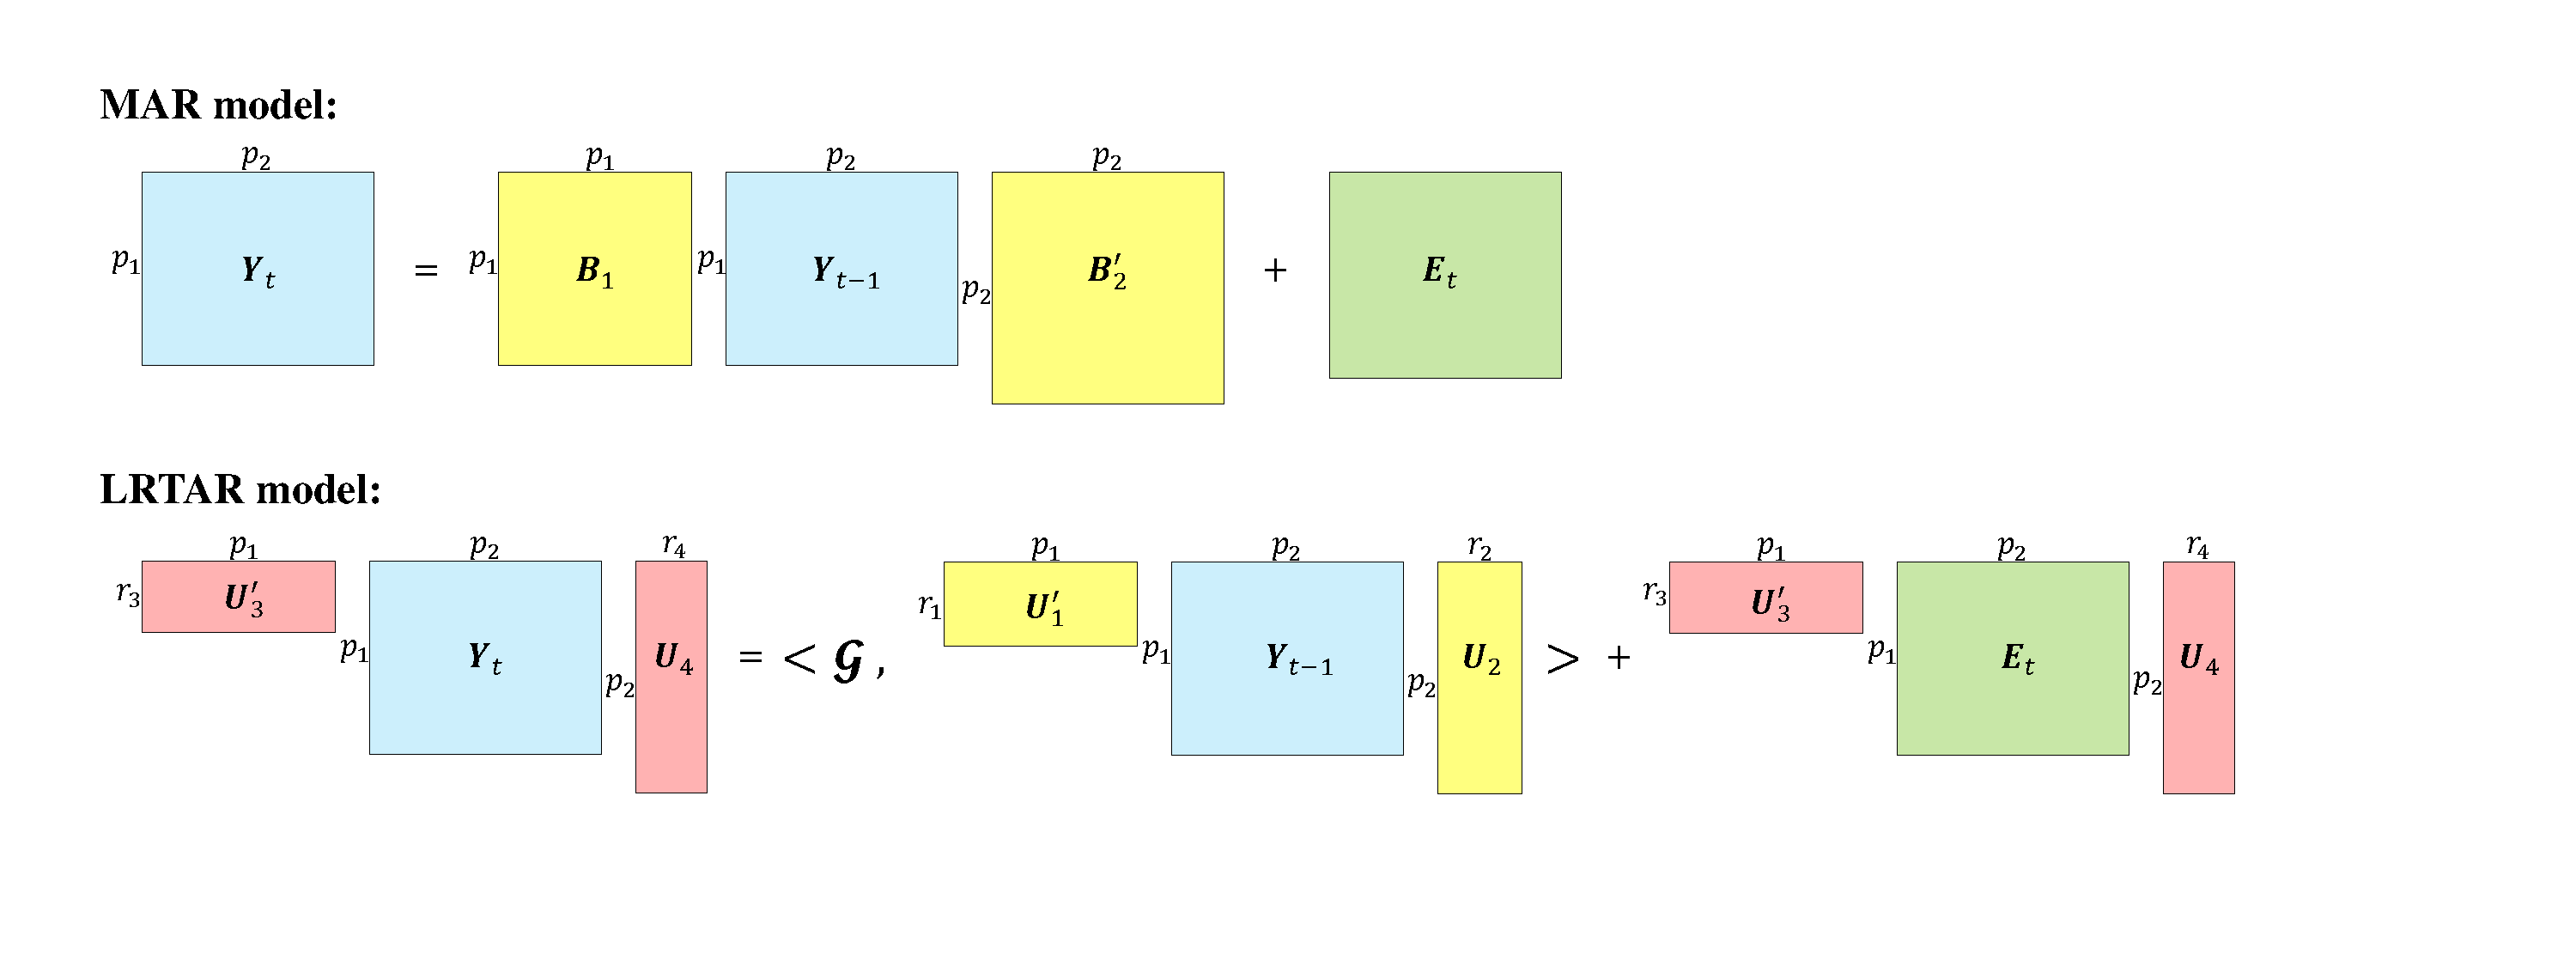
\includegraphics[width=0.95\textwidth]{Fig_TAR.pdf}
	\caption{Illustration of the MAR model and the proposed LRTAR model in the case of $d=2$.	\label{fg:Fig_TAR}}
\end{figure}


\begin{example}\label{ex2}
In the special case where $\bm{U}_{d+i}=\bm{U}_{i}$ and $r_{d+i}=r_i$ for $i=1,\dots, d$, the proposed model may be understood from the perspective of dynamic factor modeling \citep{SW11, BW16} for tensor-valued time series. Specifically, consider the following model:
\begin{equation}\label{eq:dfm_tensor}
\cm{Y}_t=\cm{F}_t\times_{i=1}^d\bm{U}_i, \quad \cm{F}_t=\langle\cm{G},\cm{F}_{t-1}\rangle+\cm{H}_t,
\end{equation}
where $\cm{Y}_t\in\mathbb{R}^{p_1\times\cdots\times p_d}$ is the observed tensor-valued time series,  $\cm{F}_t\in\mathbb{R}^{r_1\times\cdots\times r_d}$ represents $\prod_{i=1}^d r_i$ factors, and $\bm{U}_i\in\mathbb{R}^{p_i\times r_i}$ are orthonormal matrices for $i=1,\dots, d$. Here  $\cm{F}_t$ follows the tensor autoregression (TAR) with transition tensor $\cm{G}\in \mathbb{R}^{r_1\times\cdots\times r_d\times r_1\times\cdots\times r_d}$ and random error $\cm{H}_t$.
Note that \eqref{eq:dfm_tensor} can be rewritten as
\[
\cm{Y}_t =\left \langle\cm{G}\times_{i=1}^d\bm{U}_{i} \times_{i=d+1}^{2d}\bm{U}_{i},\cm{Y}_{t-1}\right \rangle+\cm{H}_t\times_{i=1}^d\bm{U}_{i}.
\]
Thus,  model \eqref{eq:dfm_tensor} is a special case of the proposed model with $\bm{U}_{d+i}=\bm{U}_{i}$ and $r_{d+i}=r_i$ for $i=1,\dots, d$, and $\cm{E}_t=\cm{H}_t\times_{i=1}^d\bm{U}_{i}$.  \citet{chen2019factor} introduces the tensor factor model in the form of $\cm{Y}_t=\cm{F}_t\times_{i=1}^d\bm{U}_i+\cm{E}_t$  without an explicit modeling of the latent factors $\cm{F}_t$. Hence, model \eqref{eq:dfm_tensor} may be regarded as a special tensor factor model with autoregressive dynamic factors, but without any random error in the model equation of $\cm{Y}_t$.
\end{example}




\section{Low-Dimensional Least Squares Estimation \label{sec:LDM}}

We consider the parameter estimation for the low-dimensional case where the sample size $T$ is sufficiently large such that the dimension of the parameter space can be assumed fixed. 
Throughout this section, we assume that the data are generated from the proposed model in Section 3, where the true transition tensor $\cm{A}$ is exactly low-Tucker rank with multilinear ranks $(r_1,\dots,r_{2d})$. This assumption will be relaxed under the high-dimensional setup in the next section.


Suppose that the true ranks $(r_1,\dots,r_{2d})$ of the exactly low-rank tensor $\cm{A}$ are known; we relegate the rank selection to Section \ref{subsec:trunc}. Then the parameters can be estimated by
\begin{equation}\label{eq:LTR}
\cm{\widehat{A}}_{\text{LTR}}=\cm{\widehat{G}}\times_{i=1}^{2d}\bm{\widehat{U}}_i=\underset{\scalebox{0.7}{\cm{G}},\bm{U}_i}{\arg\min}\sum_{t=1}^T\left\|\cm{Y}_t-\langle\cm{G}\times_{i=1}^{2d}\bm{U}_i,\cm{Y}_{t-1}\rangle\right\|_\textup{F}^2.
\end{equation}
We call $\cm{\widehat{A}}_{\text{LTR}}$ the low-Tucker-rank (LTR) estimator. Note that the minimization in \eqref{eq:LTR} is unconstrained, so the Tucker decomposition of $\cm{\widehat{A}}_{\text{LTR}}$ is not unique. Indeed, there are more than one solution of $\cm{\widehat{G}}$ and $\bm{\widehat{U}}_i$'s corresponding to the same $\cm{\widehat{A}}_{\text{LTR}}$. Due to the lack of identifiability of the Tucker decompositions, standard asymptotics of the maximum likelihood estimation cannot apply directly. Nevertheless, we  can still derive the asymptotic distribution of $\cm{\widehat{A}}_{\text{LTR}}$ using the asymptotic theory  for  overparameterized models in \cite{shapiro1986asymptotic}.


Recall that $S_1=\{1,2,\dots,d\}$ $S_2=\{d+1,d+2,\dots,2d\}$, $\bm{y}_t=\text{vec}(\cm{Y}_t)$, and $\bm{e}_t=\text{vec}(\cm{E}_t)$.
Let $\bm{\theta}=(\text{vec}(\cm{G}_{[S_2]})^\top,\text{vec}(\bm{U}_1)^\top,\cdots, \text{vec}(\bm{U}_{2d})^\top)^\top$ be the parameter vector, and  let $\bm{h}=\bm{h}(\bm{\theta})=\text{vec}(\cm{A}_{[S_2]})=\text{vec}((\otimes_{i\in S_2}\bm{U}_i)\cm{G}_{[S_2]}(\otimes_{i\in S_1}\bm{U}_i)^\top)$ be the vectorization of the transition matrix. Denote  $\bm{\Sigma}_{\bm{y}}=\text{var}(\bm{y}_t)$, $\bm{\Sigma}_{\bm{e}}=\text{var}(\bm{e}_t)$, and  $\bm{J}=\bm{\Sigma}_{\bm{e}}^{-1}\otimes\bm{\Sigma}_{\bm{y}}$. In addition, for $i=1,\dots, 2d$, let $\bm{P}_{[S_2]}^{(i)}$ be the $p^2\times p^2$ permutation matrix such that $\text{vec}(\cm{A}_{[S_2]})=\bm{P}_{[S_2]}^{(i)}\text{vec}(\cm{A}_{(i)})$. Then, it can be shown that the Jacobian matrix $\bm{H}:={\partial\bm{h}(\bm{\theta})}/{\partial\bm{\theta}}$ is given by
\begin{equation}\label{eq:H}\begin{split}
\bm{H}
=\big( &(\otimes_{i\in S_1}\bm{U}_i)\otimes(\otimes_{i\in S_2}\bm{U}_i),
\bm{P}^{(1)}_{[S_2]}\left \{\left [(\otimes_{i=1, i\neq 1}^{2d}\bm{U}_i)\cm{G}_{(1)}^\top\right ]\otimes\bm{I}_{p_1}\right \},\\
&\bm{P}^{(2)}_{[S_2]}\left \{\left [(\otimes_{i=1, i\neq 2}^{2d}\bm{U}_i)\cm{G}_{(2)}^\top\right ]\otimes\bm{I}_{p_2}\right \},\dots,
\bm{P}^{(2d)}_{[S_2]}\left \{\left [(\otimes_{i=1, i\neq 2d}^{2d}\bm{U}_i)\cm{G}_{(2d)}^\top\right ]\otimes\bm{I}_{p_{2d}}\right \}\big),
\end{split}\end{equation}
where $p_{d+i}=p_i$ for $i=1,\dots, d$.

\begin{theorem}
	\label{thm:Asymptotic}
	Suppose that the time series $\{\cm{Y}_t\}$ is generated by model \eqref{eq:LTRTAR_model} with $\mathbb{E}\|\bm{e}_t\|_2^4<\infty$, and Assumption \ref{asmp:stationary} holds. Then,
	\begin{equation}
	\sqrt{T}\textup{vec}((\cm{\widehat{A}}_{\textup{LTR}}-\cm{A})_{[S_2]})\rightarrow N(\bm{0},\bm{\bm{\Sigma}}_{\textup{LTR}}),
	\end{equation}
	in distribution as $T\rightarrow\infty$, where $\bm{\bm{\Sigma}}_{\textup{LTR}}=\bm{H}(\bm{H}^\top\bm{JH})^{\dagger}\bm{H}^\top$, and $\dagger$ is the Moore-Penrose inverse.
\end{theorem}

Since the asymptotic theory for overparameterized models in  \cite{shapiro1986asymptotic} allows for unidentifiability of the components $\cm{G}$ and $\bm{U}_i$'s in the decomposition of $\cm{A}$, Theorem \ref{thm:Asymptotic} does not require that the Tucker decomposition of $\cm{A}$ is unique; see  the proof of Theorem \ref{thm:Asymptotic}  in Appendix A for more details.

%If $\cm{G}$ and $\bm{U}_i$'s are identifiable, then, by defining $\bm{\widehat{U}}_i$ uniquely as the top $r_i$ left singular vectors of $(\cm{\widehat{A}}_{\textup{LTR}})_{(i)}$ such that the first nonzero element in each of its columns is positive, for $i=1, \dots, d$, and $\cm{\widehat{G}}=\cm{\widehat{A}}_{\textup{LTR}}\times_{i=1}^d\bm{\widehat{U}}_i^\top$, we further have the following asymptotic results for $\cm{\widehat{G}}$ and $\bm{\widehat{U}}_i$'s. 

%\begin{corollary} \label{cor:Asymptotic2}
%	Suppose that the conditions of Theorem \ref{thm:Asymptotic} and Assumption \ref{asmp:identify} hold. Then $\sqrt{T}\textup{vec}(\cm{\widehat{G}}-\cm{G})$ and $\sqrt{T}\textup{vec}(\bm{\widehat{U}}_i-\bm{U}_i)$ converge to normal distributions for $i=1,\dots,2d$ as $T\to\infty$.
%\end{corollary}


Next we compare the result in Theorem \ref{thm:Asymptotic} to those of two other consistent estimators for the proposed model in the low-dimensional setup. Note that the rank of $\cm{A}_{[S_2]}$ in \eqref{eq:VAR_rep} is at most $s_1:=\min(\prod_{i=1}^dr_i,\prod_{i=d+1}^{2d}r_i)$. Thus, $\cm{A}_{[S_2]}$ can be estimated by both
the reduced-rank regression (RRR) and ordinary least squares (OLS) methods,
\begin{equation}\label{eq:RRR}
\cm{\widehat{A}}_{\text{RRR}}=\underset{\text{rank}(\scalebox{0.7}{\cm{B}}_{[S_2]})\leq s_1}{\argmin}~\frac{1}{T}\sum_{t=1}^T\|\cm{Y}_t-\langle\cm{B},\cm{Y}_{t-1}\rangle\|_\text{F}^2
\end{equation}
and
\begin{equation*}
\cm{\widehat{A}}_{\text{OLS}}=\underset{\scalebox{0.7}{\cm{B}}}{\argmin}~\frac{1}{T}\sum_{t=1}^T\|\cm{Y}_t-\langle\cm{B},\cm{Y}_{t-1}\rangle\|_\text{F}^2.
\end{equation*}
Naturally, under model \eqref{eq:LTRTAR_model},  $\cm{\widehat{A}}_{\text{LTR}}$ is asymptotically more efficient than $\cm{\widehat{A}}_{\textup{RRR}}$ and $\cm{\widehat{A}}_{\textup{OLS}}$:

\begin{corollary}
	\label{cor:OLSRRR}
	If the conditions of Theorem \ref{thm:Asymptotic} hold, then $\sqrt{T}\textup{vec}((\cm{\widehat{A}}_{\textup{OLS}}-\cm{A})_{[S_2]})\to N(0,\bm{\Sigma}_{\textup{OLS}})$ and $\sqrt{T}\textup{vec}((\cm{\widehat{A}}_{\textup{RRR}}-\cm{A})_{[S_2]})\to N(0,\bm{\Sigma}_{\textup{RRR}})$ in distribution as $T\to\infty$. Moreover, it holds that $\bm{\Sigma}_{\textup{LTR}}\leq\bm{\Sigma}_{\textup{RRR}}\leq\bm{\Sigma}_{\textup{OLS}}$.
\end{corollary}

To solve the minimization problem in \eqref{eq:LTR}, we propose an alternating least squares (ALS) method. Specifically, by the vector representation  of the proposed model in \eqref{eq:VAR_rep}, the loss function in \eqref{eq:LTR} can be rewritten as
\[
L(\cm{G}, \bm{U}_1, \dots, \bm{U}_{2d})=\sum_{t=1}^T\Big\|\bm{y}_t-(\otimes_{i\in S_2}\bm{U}_i)\cm{G}_{[S_2]}(\otimes_{i\in S_1}\bm{U}_i)^\top\bm{y}_{t-1}\Big\|_2^2=\sum_{t=1}^T\Big\|\bm{y}_t-\bm{m}(\bm{\theta})\Big\|_2^2,
\]
where $\bm{m}(\bm{\theta})=(\otimes_{i\in S_2}\bm{U}_i)\cm{G}_{[S_2]}(\otimes_{i\in S_1}\bm{U}_i)^\top\bm{y}_{t-1}$ is the conditional mean of $\bm{y}_t=\text{vec}(\cm{Y}_t)$ and is a function of the parameter vector $\bm{\theta}=(\bm{\theta}_0^\top,\bm{\theta}_1^\top,\dots, \bm{\theta}_{2d}^\top)^\top$, with $\bm{\theta}_0=\text{vec}(\cm{G}_{[S_2]})$ and $\bm{\theta}_i=\text{vec}(\bm{U}_{i})$ for $i=1,\dots, 2d$.
Note that $\bm{m}(\bm{\theta})$ is linear in each $\bm{\theta}_i$ while keeping the other components $\bm{\theta}_j$ with $0\leq j\neq i \leq 2d$ fixed.  This is indeed because 
\begin{align}
\bm{m}(\bm{\theta})&=(\otimes_{i\in S_2}\bm{U}_i)\cm{G}_{[S_2]}\bm{P}_{k,1}\left\{\left[(\otimes_{i\in S_1,i\neq k}\bm{U}_i)^\top(\cm{Y}_{t-1})_{(k)}^\top\right]\otimes \bm{I}_{r_k}\right\}\bm{P}_{k,3}\text{vec}(\bm{U}_k)\\
&=\bm{P}_{k,2}\left\{\left[(\otimes_{i\in S_2,i\neq d+k}\bm{U}_{i})(\cm{M}_{t-1})_{(k)}^\top\right]\otimes\bm{I}_{p_{k}}\right\}\text{vec}(\bm{U}_{d+k})\\
&=\left\{\left[\bm{y}_{t-1}^\top(\otimes_{i\in S_1}\bm{U}_i)\right]\otimes(\otimes_{i\in S_2}\bm{U}_i)\right\}\text{vec}(\cm{G}_{[S_2]}),
\end{align}
for $k=1,\dots, d$, where $\bm{P}_{k,1}\in\mathbb{R}^{\prod_{i=1}^dr_i\times\prod_{i=1}^dr_i}$, $\bm{P}_{k,2}\in\mathbb{R}^{p\times p}$ and $\bm{P}_{k,3}\in\mathbb{R}^{r_kp_k\times r_kp_k}$ are permutation matrices defined such that $\bm{P}_{k,1}\text{vec}(\cm{T}_{(k)})=\text{vec}(\cm{T})$ for any  $\cm{T}\in\mathbb{R}^{r_1\times\cdots\times r_d}$,   $\bm{P}_{k,2}\text{vec}(\cm{T}_{(k)})=\text{vec}(\cm{T})$ for any $\cm{T}\in\mathbb{R}^{p_1\times\cdots\times p_d}$, and   $\bm{P}_{k,3}\text{vec}(\bm{U}_{k})=\text{vec}(\bm{U}_{k}^\top)$, and $\cm{M}_{t-1}\in\mathbb{R}^{r_{d+1}\times\cdots\times r_{2d}}$ is defined such that $\text{vec}(\cm{M}_t)=\cm{G}_{[S_2]}(\otimes_{i\in S_1}\bm{U}_i)^\top\bm{y}_{t-1}$. Therefore, we can update each component parameter vector $\bm{\theta}_i$, and hence the corresponding $\cm{G}$ and $\bm{U}_i$'s, iteratively by the least squares method.  The resulting ALS algorithm is shown in Algorithm  \ref{alg:LSE}.

\begin{algorithm}[t]
  \caption{ALS algorithm for LTR estimator}
  \label{alg:LSE}
    Initialize: $\cm{A}^{(0)}=\cm{\widehat{A}}_{\textup{RRR}}$ or $\cm{\widehat{A}}_{\textup{OLS}}$\\ HOSVD: $\cm{A}^{(0)}\approx\cm{G}^{(0)}\times_{i=1}^{2d}\bm{U}_i^{(0)}$,~~with multilinear ranks $(r_1,\dots,r_{2d})$.\\
    \textbf{repeat} $s=0,1,2,\dots$\\
    \hspace*{0.5cm}\textbf{for} $k=1,\dots,d$\\
    \hspace*{1cm}$\bm{U}_k^{(s+1)}\leftarrow\underset{\bm{U}_k}{\arg\min}\sum_{t=1}^T\Big\|\bm{y}_t-(\otimes_{i\in S_2}\bm{U}_i^{(s)})\cm{G}_{[S_2]}\bm{P}_{k,1}  \left\{\left[(\otimes_{i\in S_1,i\neq k}\bm{U}_i^{(s)})^\top(\cm{Y}_{t-1})_{(k)}^\top\right]\otimes \bm{I}_{r_k}\right\}$\\
    \hspace*{5.5cm}$\text{vec}(\bm{U}_k)\Big\|_2^2$\\
    \hspace*{0.5cm}\textbf{end for}\\
    \hspace*{0.5cm}\textbf{for} $k=1,\dots,d$\\
    \hspace*{1cm}$\bm{U}_{d+k}^{(s+1)}\leftarrow\underset{\bm{U}_{d+k}}{\arg\min}\sum_{t=1}^T\Big\|\bm{y}_t-\bm{P}_{k,2}\big\{\left[(\otimes_{i\in S_2,i\neq d+k}\bm{U}_{i}^{(s)}) (\cm{M}^{(s+1)}_{t-1})_{(k)}^\top\right]\otimes\bm{I}_{p_{k}}\big\}\text{vec}(\bm{U}_{d+k})\Big\|_2^2$\\
    \hspace*{0.5cm}\textbf{end for}\\
    \hspace*{0.5cm}$\cm{G}^{(s+1)}\leftarrow \underset{\scalebox{0.75}{\cm{G}}}{\arg\min}\sum_{t=1}^T\Big\|\bm{y}_t-\left\{\left[\bm{y}_{t-1}^\top(\otimes_{i\in S_1}\bm{U}_i^{(s+1)})\right]\otimes(\otimes_{i\in S_2}\bm{U}_i^{(s+1)})\right\}\text{vec}(\cm{G}_{[S_2]})\Big\|_2^2$\\
    \hspace*{0.5cm}$\cm{A}^{(s+1)}\leftarrow\cm{G}^{(s+1)}\times_{i=1}^{2d}\bm{U}_i^{(s+1)}$\\
    \textbf{until convergence}
\end{algorithm}

As mentioned, the minimization in \eqref{eq:LTR} is unconstrained. Accordingly, to obtain $\cm{\widehat{A}}_{\text{LTR}}$, no orthogonality constraint of $\cm{G}$ and $\bm{U}_i$'s is needed in Algorithm \ref{alg:LSE}. Instead, we compute the final unique estimates of $\cm{\widehat{G}}$ and $\bm{\widehat{U}}_i$'s  by the  HOSVD operation based on the unconstrained solution $\cm{\widehat{A}}_{\text{LTR}}$ obtained from  Algorithm \ref{alg:LSE}. Specifically, we compute each $\bm{\widehat{U}}_i$ uniquely as the top $r_i$ left singular vectors of $(\cm{\widehat{A}}_{\text{LTR}})_{(i)}$ such that the first element in each column of $\bm{\widehat{U}}_i$ is positive, and set $\cm{\widehat{G}}=[\![\cm{\widehat{A}}_{\text{LTR}};\bm{\widehat{U}}_1^\top,\cdots,\bm{\widehat{U}}_{2d}^\top]\!]$. Similar alternating algorithms without imposing identification constraints can be found in the literature of tensor decomposition; see, e.g. \citet{Zhou13} and \citet{li2018tucker}.

%\subsection{Rank selection by BIC}
%
%The LTR estimator is defined with prespecified Tucker ranks $(r_1,\dots,r_{2d})$ and the asymptotic theory is established based on the correct Tucker ranks. We propose to select multilinear ranks $r_i$s based on the information criteria. The degrees of freedom of the low-Tucker-rank estimator can be defined as the number of free parameters in the Tucker decomposition, namely $\text{df}=\prod_{i=1}^{2d}r_i+\sum_{i=1}^{2d}r_i(p_i-r_i)$. Therefore, one can apply the BIC to select the multilinear ranks.
%
%In Section 4, we propose a truncated regularized estimator and rank selection consistency is shown under some conditions. In low-dimensional case, we can apply this approach to select the Tucker ranks as well.


\section{High-Dimensional Regularized Estimation\label{sec:HDM}}

\subsection{Regularization via One-Mode Matricization \label{subsec:1mode}}
The methods in the previous section rely on the assumptions that the dimension is fixed and that the true transition tensor is exactly low-rank with known Tucker ranks. We next relax both assumptions.  Specifically, under the high-dimensional setup, we consider regularized estimation of model \eqref{eq:LTRTAR_model} via different nuclear-norm-type penalties and develop the corresponding non-asymptotic theory under only an approximately low-Tucker-rank assumption on the  underlying true transition tensor.

In model \eqref{eq:LTRTAR_model}, the exactly low-rank transition tensor $\cm{A}\in\mathbb{R}^{p_1\times\cdots\times p_{2d}}$  is subject to the constraints $r_i=\text{rank}(\cm{A}_{(i)})$, for $i=1,\dots, 2d$. A commonly used convex relaxation of such multilinear rank constraints is the regularization via the sum of nuclear (SN) norms of all the one-mode matricizations,
\begin{equation}\label{eq:SN_norm}
\|\cm{A}\|_{\text{SN}}=\sum_{i=1}^{2d}\|\cm{A}_{(i)}\|_*.
\end{equation}
The SN norm has been widely used in the literature  \citep{gandy2011tensor, tomioka2011statistical, liu2013tensor, raskutti2019convex} to simultaneously encourage the low-rankness for all modes of a tensor. 
This leads us to the SN norm regularized estimator
\begin{equation}
\cm{\widehat{A}}_{\text{SN}}=\underset{\scalebox{0.7}{\cm{A}}}{\argmin}\left\{\frac{1}{T}\sum_{t=1}^T\|\cm{Y}_t-\langle\cm{A},\cm{Y}_{t-1}\rangle\|_\text{F}^2+\lambda_{\textup{SN}}\|\cm{A}\|_{\text{SN}}\right\},
\end{equation}
where $\lambda_{\text{SN}}$ is the tuning parameter. Note that if instead of  $\|\cm{A}\|_{\text{SN}}$, only one single nuclear norm, say $\|\cm{A}_{(1)}\|_*$, is penalized, then the resulting estimator will only enforce the low-rankness for the first mode of $\cm{A}$,  while failing to do so for all the other $2d-1$ modes, and hence will be less efficient than the above SN estimator.

To derive the estimation error bound for $\cm{\widehat{A}}_{\text{SN}}$, we make the following assumption on the random error $\bm{e}_t=\textup{vec}(\cm{E}_t)$.

\begin{assumption}
	\label{asmp:gaussian}
	Let $\bm{e}_t=\bm{\Sigma}_{\bm{e}}^{1/2}\bm{\xi}_t$, where $\{\bm{\xi}_t\}$ is a sequence of $i.i.d.$ random vectors, with $\mathbb{E}(\bm{\xi}_t)=\bm{0}$ and $\textup{var}(\bm{\xi}_t)=\bm{I}_p$, and $\bm{\Sigma_e}=\textup{var}(\bm{e}_t)$ is  a positive definite matrix. In addition, the entries $(\bm{\xi}_{it})_{1\leq i\leq p}$ of  $\bm{\xi}_t$ are mutually independent and $\kappa^2$-sub-Gaussian, i.e.,
	$\mathbb{E}(e^{\mu\xi_{it}})\leq e^{\kappa^2\mu^2/2}$, for any $\mu\in\mathbb{R}$ and  $i=1,\dots, p$.
\end{assumption}

The sub-Gaussianity condition in Assumption \ref{asmp:gaussian} is milder than the  commonly used normality assumption in the literature  on high-dimensional stationary vector autoregressive models \citep{basu2015regularized, raskutti2019convex}. This relaxation is made possible through establishing a novel martingale-based concentration bound in the proof of the deviation bound; see Lemma \ref{lemma:deviation} in Appendix \ref{subsec:auxlemma}. The covariance matrix $\bm{\Sigma_e}$ captures the contemporaneous dependency in $\cm{E}_t$, and the constant $\kappa$ controls the tail heaviness of the marginal distributions.

For any $z\in\mathbb{C}$, let $\mathcal{A}(z)=\bm{I}_{p}-\cm{A}_{[S_2]}z$ be a matrix polynomial, where $\mathbb{C}$ is the set of complex numbers. Let
$\mu_{\min}(\mathcal{A})=\underset{|z|=1}{\min}\,\lambda_{\min}(\mathcal{A}^*(z)\mathcal{A}(z))$ and $\mu_{\max}(\mathcal{A})=\underset{|z|=1}{\max}\,\lambda_{\max}(\mathcal{A}^*(z)\mathcal{A}(z))$, where $\mathcal{A}^*(z)$ is the conjugate transpose of $\mathcal{A}(z)$; see \cite{basu2015regularized} for more discussions on the connection between the spectral density of the VAR process and the two quantities. In addition, let
\[
\alpha_{\textup{RSC}}=\frac{\lambda_{\min}(\bm{\Sigma_e})}{\mu_{\max}(\mathcal{A})}, \quad M_1=\frac{\lambda_{\max}(\bm{\Sigma_e})}{\mu^{1/2}_{\min}(\mathcal{A})}, \quad\text{and}\quad M_2=\frac{\lambda_{\min}(\bm{\Sigma}_{\bm{e}})\mu_{\max}(\mathcal{A})}{\lambda_{\max}(\bm{\Sigma_e})\mu_{\min}(\mathcal{A})}.
\]

The exactly low-rankness of the true transition tensor $\cm{A}$ assumed in Section \ref{sec:LDM}  could be too stringent in real-world applications. In what follows, we relax it to  the following approximately low-rank assumption:	We assume that all one-mode matricizations of the underlying true transition tensor $\cm{A}$ belong to the set of approximately low-rank matrices, namely $\cm{A}_{(i)}\in\mathbb{B}_q(r_q^{(i)};p_i,p_{-i}p)$ for some $q\in[0,1)$, where
\begin{equation}
	\mathbb{B}_q(r;d_1,d_2):=\left\{\bm{M}\in\mathbb{R}^{d_1\times d_2}:\sum_{i=1}^{\min(d_1,d_2)}\sigma_i(\bm{M})^q\leq r\right\},
\end{equation}
and $p_{-i}=p/p_i=\prod_{j=1,j\neq i}^{d}p_j$. For the convenience of notation, here we require that $0^0=0$. Note that when $q=0$, $\mathbb{B}_0(r;d_1,d_2)$ is the set of $d_1$-by-$d_2$ rank-$r$ matrices. For $q>0$, the restriction on $\sum_{i=1}^{\min(d_1,d_2)}\sigma_i(\bm{M})^q\leq r$ requires that the singular values decay fast, and it is more general and natural than the exactly low-rank assumption.



% $\alpha_{\textup{RSC}}=\lambda_{\min}(\bm{\Sigma_e})/\mu_{\max}(\mathcal{A})$, $M_1=\lambda_{\max}(\bm{\Sigma_e})/\mu^{1/2}_{\min}(\mathcal{A})$, and $M_2=[\lambda_{\min}(\bm{\Sigma}_{\bm{e}})\mu_{\min}(\mathcal{A})]/[\lambda_{\max}(\bm{\Sigma_e})\mu_{\max}(\mathcal{A})]$.

%$\mu_{\min}(\mathcal{A})=\underset{\theta\in[-\pi,\pi]}{\min}\lambda_{\min}((\bm{I}_p-\cm{A}_{[S_2]}'e^{i\theta})(\bm{I}_p-\cm{A}_{[S_2]}'e^{-i\theta}))$ and
%$\mu_{\max}(\mathcal{A})=\underset{\theta\in[-\pi,\pi]}{\max}\lambda_{\min}((\bm{I}_p-\cm{A}_{[S_2]}'e^{i\theta})(\bm{I}_p-\cm{A}_{[S_2]}'e^{-i\theta}))$


\begin{theorem} \label{thm:SN}
Under Assumptions \ref{asmp:stationary} and \ref{asmp:gaussian}, if $T\gtrsim \max_{1\leq i\leq d}p_{-i}p+\max(\kappa^2,\kappa^4)M_2^{-2}p$, $\lambda_{\textup{SN}}\gtrsim\kappa^2M_1d^{-2}\sum_{i=1}^{d}\sqrt{ p_{-i} p/T}$, and $\cm{A}_{(i)}\in\mathbb{B}_q(r_q^{(i)};p_i,p_{-i}p)$ for some $q\in[0,1)$ and all $i=1,\dots,2d$, then with probability at least $1-2\sum_{i=1}^{d}\exp(-Cp_{-i}p)-\exp[-C\min(\kappa^{-2},\kappa^{-4})M_2^2p]$,
	\begin{equation}
		\|\cm{\widehat{A}}_{\textup{SN}}-\cm{A}\|_{\textup{F}}\lesssim\sqrt{r_q}\left(\frac{2d\cdot\lambda_{\textup{SN}}}{\alpha_{\textup{RSC}}}\right)^{1-q/2}
	\end{equation}
	where $r_q=(2d)^{-1}\sum_{i=1}^{2d}r_q^{(i)}$.	
\end{theorem}


By Theorem \ref{thm:SN}, when $\lambda_{\textup{SN}}\asymp\kappa^2M_1d^{-2}\sum_{i=1}^{d}\sqrt{p_{-i} p/T}$, the estimation error bound scales as
$\sqrt{r_q}(\max_{1\leq i\leq d}p_{-i}p/T)^{1/2-q/4}$; note that the factor $d$ in the error bounds is canceled by the $d^{-2}$ in the rate of $\lambda_{\textup{SN}}$. When $q=0$, namely $\cm{A}$ is exactly low-rank with Tucker ranks $(r_0^{(1)},\dots,r_0^{(2d)})$, the error bound reduces to $\sqrt{r_0\max_{1\leq i\leq d}p_{-i}p/T}$ and it is comparable to that in \citet{tomioka2011statistical} for $i.i.d.$ tensor regression. 

However, recent research \citep[e.g.,][]{mu2014square,raskutti2019convex} has shown that the SN norm regularization approach is suboptimal, mainly because $\cm{A}_{(i)}$ is an unbalanced \textit{fat-and-short} matricization of a higher-order tensor.  Technically, in the proof of Theorem \ref{thm:SN}, an essential intermediate step is to establish the deviation bound, where we need to upper bound the operator norm of a sub-Gaussian random matrix with the same dimensions as $\cm{A}_{(i)}$; see  Lemma \ref{lemma:deviation} in Appendix \ref{subsec:lemma} for details. Undesirably,  the order of this operator norm  will be dominated by the larger of the  row and column dimensions of the matrix $\cm{A}_{(i)}\in\mathbb{R}^{p_i \times p_{-i}p}$, and hence by the column dimension $p_{-i}p$, which eventually appears in the  error bound.  This indicates that the imbalance of the matricization leads to the efficiency bottleneck of the SN estimator.


On the other hand, similarly to \eqref{eq:RRR}, since the the reduced-rank VAR  model can be regarded as an overparameterization of the proposed LRTAR model, alternatively one may focus on the approximately low-rank structure of the transition matrix $\cm{A}_{[S_2]}$ in the VAR representation in \eqref{eq:VAR_rep}, and adopt the matrix nuclear (MN)  estimator \citep{negahban2011estimation} to estimate $\cm{A}$,
\begin{equation}\label{eq:matrixnuclear}
\cm{\widehat{A}}_{\text{MN}}=\underset{\scalebox{0.7}{\cm{A}}}{\argmin}\left\{\frac{1}{T}\sum_{t=1}^T\|\cm{Y}_t-\langle\cm{A},\cm{Y}_{t-1}\rangle\|_\text{F}^2+\lambda_{\textup{MN}}\|\cm{A}_{[S_1]}\|_*\right\}.
\end{equation}
Note that the multi-mode matricization $\cm{A}_{[S_2]}=\cm{A}_{[S_1]}^\top$ is a $p\times p$ square matrix. Thus, the loss of efficiency due to the unbalanced matricization can be avoided, which is confirmed by the following theorem.

\begin{theorem}\label{thm:MN}
Under Assumptions \ref{asmp:stationary} and \ref{asmp:gaussian}, if $T\gtrsim [1+\max(\kappa^2,\kappa^4)M_2^{-2}]p$, $\lambda_{\textup{MN}}\gtrsim\kappa^2M_1\sqrt{p/T}$, and $\cm{A}_{[S_1]}\in\mathbb{B}_q(s_q^{(1)};p,p)$ for some $q=[0,1)$, then with probability at least $1-\exp(-Cp)-\exp[-C\min(\kappa^{-2},\kappa^{-4})M_2^2p]$,
	\begin{equation*}
	\|\cm{\widehat{A}}_{\textup{MN}}-\cm{A}\|_{\textup{F}}\lesssim\sqrt{s_q^{(1)}}\left(\frac{\lambda_{\textup{MN}}}{\alpha_{\textup{RSC}}}\right)^{1-q/2}.
	\end{equation*}
\end{theorem}

Theorem \ref{thm:MN} shows that, with  $\lambda_{\textup{MN}}\asymp\kappa^2M_1\sqrt{p/T}$, the estimation error bound for $\cm{\widehat{A}}_{\text{MN}}$ scales as $\sqrt{s_q^{(1)}}(p/T)^{1/2-q/4}$. This result is comparable to that in \citet{negahban2011estimation} for reduced-rank VAR models, yet we relax both the constraint $\|\bm{A}\|_{\text{op}}<1$ on the transition matrix $\bm{A}$ and the normality assumption on the random error in their paper. This estimation error bound is clearly smaller than that in Theorem \ref{thm:SN}, as $(\max_{1\leq i\leq d}p_{-i}p/T)^{1/2-q/4}$ in general can be much larger than $(p/T)^{1/2-q/4}$ when $s_q^{(1)}\asymp r_q$. Therefore, adopting square matricization can indeed improve the estimation performance. 

The idea of using square matricization to improve efficiency was adopted by \citet{mu2014square} in low-rank tensor completion problems. Their proposed method, called the square deal, is to first unfold a general higher-order tensor into a matrix with similar numbers of rows and columns, and then use the MN norm as the regularizer. However, for our estimation problem, despite the advantage of $\cm{\widehat{A}}_{\textup{MN}}$  over $\cm{\widehat{A}}_{\textup{SN}}$, Theorem \ref{thm:MN} reveals another drawback of $\cm{\widehat{A}}_{\textup{MN}}$. 
That is, the  error bounds for $\cm{\widehat{A}}_{\textup{MN}}$  depend on the $\ell_q$ radius $s_q^{(1)}$ of the singular values of $\cm{A}_{[S_1]}$, suggesting that $\cm{\widehat{A}}_{\textup{MN}}$ may perform badly when $s_q^{(1)}$ is relatively large.  
In other words, unless we have prior knowledge that the $\ell_q$ ``norm'' of singular values of particular matricization $\cm{A}_{[S_1]}$ is truly small, $\cm{\widehat{A}}_{\textup{MN}}$ may not be desirable in practice. 

On the other hand, although the SN regularizer in \eqref{eq:SN_norm} suffers from  inefficiency due to the imbalance of one-mode matricizations,  it has the attractive feature of simultaneously enforcing the low-rankness across all modes of the tensor $\cm{A}$, and thus is more  efficient than its counterpart which considers only one single one-mode matricization, say, $\|\cm{A}_{(1)}\|_*$. Similarly, if we can enforce the approximate low-rankness across all possible square matricizations of $\cm{A}$, the estimation performance may be further improved upon $\cm{\widehat{A}}_{\textup{MN}}$.  This motivates us to propose  a new regularization approach in the next subsection.

\begin{comment}
\subsection{Regularization via Square Matricization}

In this subsection, we propose a novel convex regularizer which improves upon both the SN and MN regularizers in \eqref{eq:SN_norm} and \eqref{eq:matrixnuclear}, respectively, by simultaneously encouraging the low-rankness across all possible square matricizations of the transition tensor $\cm{A}$.

For any $2d$-th-order tensor $\cm{A}\in\mathbb{R}^{p_1\times\cdots\times p_{d}\times p_1\times\cdots\times p_{d}}$, its multi-mode matricization $\cm{A}_{[I]}$ will be a $p\times p$ square  matrix, with $p=\prod_{i=1}^{d}p_i$, if the index set is  chosen as \[I=\{\ell_1,\dots, \ell_d\},\] 
where each index $\ell_i$ is set to either $i$ or $d+i$,  for $i=1,\dots, d$.  For instance, $\cm{A}_{[S_1]}$ is the square matricization formed by setting $\ell_i=i$ for all $i=1,\dots, d$.  Moreover, if $\cm{A}$ has multilinear ranks $(r_1,\dots,r_{2d})$, then the rank of the matricization $\cm{A}_{[I]}$ is  at most $\min(\prod_{i=1,i\in I}^{2d}r_i,\prod_{i=1,i\notin I}^{2d}r_i)$. Motivated by \citet{tomioka2013convex}, we consider the latent square-matrix nuclear (LSN) norm and the resulting estimator would enjoy the efficiency gain from both the use of square matricizations and simultaneous incorporation of many rank constraints.

Obviously, there are $2^d$ possible choices of the index set $I$ that corresponds to a square matricization $\cm{A}_{[I]}$. However, since $\cm{A}_{[I]}=\cm{A}_{[I^\complement]}^\top$, when defining the LSN norm, we only need to include one of $I$ and its complement $I^\complement$. A simple way to do so is to choose only sets containing the index one. That is, fix $\ell_1=1$ and choose  $\ell_i=i$ or  $d+i$ for $i=2,\dots, d$. This results in totally $K:=2^{d-1}$ chosen index sets, denoted by $I_1,I_2,\dots,I_{K}$. Note that $I_1=S_1=\{1,\dots, d\}$. For example, when $d=3$, we have four chosen index sets, $I_1=\{1,2,3\}, I_2=\{1,5,3\}, I_3=\{1,2,6\}$ and $I_4=\{1,5,6\}$.

Based on the above choice of the $K$ index sets, we introduce the following LSN norm
\begin{equation}
	\label{eq:LSN_norm}
	\|\cm{A}\|_\text{LSN} = \inf_{\scalebox{0.75}{$\cm{A}^{(1)}+\cdots+\cm{A}^{(K)}=\cm{A}$}}\left(\sum_{k=1}^{K}\|\cm{A}^{(k)}_{[I_k]}\|_*\right),
\end{equation}
where the infimum is taken over all components $\cm{A}^{(1)},\dots,\cm{A}^{(K)}$ that sum to $\cm{A}$. The corresponding estimator is defined as
\begin{equation}
	\label{eq:LSN_est}
	\cm{\widehat{A}}_\text{LSN}=\underset{\scalebox{0.75}{\cm{A}}}{\argmin}\left\{\frac{1}{T}\sum_{t=1}^T\|\cm{Y}_t-\langle\cm{A},\cm{Y}_{t-1}\rangle\|_\text{F}^2+\lambda_\text{LSN}\|\cm{A}\|_\text{LSN}\right\},
\end{equation}
where $\lambda_\text{LSN}$ is the regularization parameter.

For each square matricization $\cm{A}_{[I_k]}$, denote $s_k^*=\text{rank}(\bm{A}_{[I_k]})$. If each $\text{rank}(\bm{A}_{(i)})=r_i$, for all $1\leq i\leq 2d$, we can check that $s_k^*\leq s_k:=\min(\prod_{i,i\in I_k}^{2d}r_i,\prod_{i,i\not\in I_k}^{2d}r_i)$. Similarly, if all $\cm{A}_{(i)}$'s are approximately low-rank, the square matricizations $\cm{A}_{[I_k]}$ are also approximately low-rank. In contrast to the SN norm in \eqref{eq:SN_norm} which directly matches the multilinear ranks, the LSN norm encourages the multilinear low-rank structure of $\cm{A}$ by simultaneously enforcing the low-rankness of all the square matricization $\cm{A}_{[I_k]}$. The following theorem gives the theoretical results for $\cm{\widehat{A}}_\text{LSN}$.
\end{comment}

\subsection{Regularization via Square Matricization \label{subsec:sqrmode}}
In this subsection, we propose a novel convex regularizer which improves upon both the SN and MN regularizers in \eqref{eq:SN_norm} and \eqref{eq:matrixnuclear}, respectively, by simultaneously encouraging the low-rankness across all possible square matricizations of the transition tensor $\cm{A}$.

For any $2d$-th-order tensor $\cm{A}\in\mathbb{R}^{p_1\times\cdots\times p_{d}\times p_1\times\cdots\times p_{d}}$, its multi-mode matricization $\cm{A}_{[I]}$ will be a $p\times p$ square  matrix, with $p=\prod_{i=1}^{d}p_i$, if the index set is  chosen as \[I=\{\ell_1,\dots, \ell_d\},\] 
where each index $\ell_i$ is set to either $i$ or $d+i$,  for $i=1,\dots, d$.  For instance, $\cm{A}_{[S_1]}$ is the square matricization formed by setting $\ell_i=i$ for all $i=1,\dots, d$.  Moreover, if $\cm{A}$ has multilinear ranks $(r_1,\dots,r_{2d})$, then the rank of the matricization $\cm{A}_{[I]}$ is  at most $\min(\prod_{i=1,i\in I}^{2d}r_i,\prod_{i=1,i\notin I}^{2d}r_i)$. Therefore, if we penalize the sum of nuclear norms of all such squares matricizations, which we call the sum of square-matrix nuclear (SSN) norms for simplicity, then the resulting estimator would  enjoy the efficiency gain from both  the use of square matricizations and simultaneous  incorporation of many rank constraints.


Obviously, there are $2^d$ possible choices of the index set $I$ that corresponds to a square matricization $\cm{A}_{[I]}$. However, since $\cm{A}_{[I]}=\cm{A}_{[I^\complement]}^\top$, when defining the SSN norm, we only need to include one of $I$ and its complement $I^\complement$. A simple way to do so is to choose only sets containing the index one. That is, fix $\ell_1=1$ and choose  $\ell_i=i$ or  $d+i$ for $i=2,\dots, d$. This results in totally $2^{d-1}$ chosen index sets, denoted by $I_1,I_2,\dots,I_{2^{d-1}}$. Note that $I_1=S_1=\{1,\dots, d\}$. For example, when $d=3$, we have four chosen index sets, $I_1=\{1,2,3\}, I_2=\{1,5,3\}, I_3=\{1,2,6\}$ and $I_4=\{1,5,6\}$.


Based on the above choice of the $2^{d-1}$ index sets,  we introduce the following SSN norm,
\begin{equation} \label{eq:SSN_norm}
\|\cm{A}\|_{\text{SSN}}=\sum_{k=1}^{2^{d-1}}\left\|\cm{A}_{[I_k]}\right\|_*.
\end{equation}
The corresponding estimator is defined as
\begin{equation}\label{eq:SSN_est}
\cm{\widehat{A}}_{\text{SSN}}=\underset{\scalebox{0.7}{\cm{A}}}{\argmin}\left\{\frac{1}{T}\sum_{t=1}^T\|\cm{Y}_t-\langle\cm{A},\cm{Y}_{t-1}\rangle\|_\text{F}^2+\lambda_{\textup{SSN}}\|\cm{A}\|_{\text{SSN}}\right\},
\end{equation}
where $\lambda_{\textup{SSN}}$ is the tuning parameter. 

If the rank of one-mode matricizations $\text{rank}(\cm{A}_{(i)})=r_i$, each square matricization $\cm{A}_{[I_k]}$ is also low-rank with $\text{rank}(\cm{A}_{[I_k]})\leq\min(\prod_{i=1,i\in I_k}^{2d}r_i,\prod_{i=1,i\notin I_k}^{2d}r_i)$. Similarly, if all $\cm{A}_{(i)}$s are approximately low-rank, the square matricizations are approximately low-rank as well. In contrast to the SN norm in \eqref{eq:SN_norm} which directly matches the multilinear ranks $\text{rank}(\cm{A}_{(i)})$ for $i=1,\dots, d$,  the SSN norm encourages the multilinear low-rank structure of $\cm{A}$ by simultaneously enforcing the low-rankness of all the square matricizations $\cm{A}_{[I_k]}$.
The following theorem gives the theoretical results for $\cm{\widehat{A}}_{\text{SSN}}$.

\begin{theorem} \label{thm:SSN}
Under Assumptions \ref{asmp:stationary} and \ref{asmp:gaussian}, if $T\gtrsim [1+\max(\kappa^2,\kappa^4)M_2^{-2}]p$, $\lambda_{\textup{SSN}}\gtrsim\kappa^2M_12^{1-d}\sqrt{p/T}$, and $\cm{A}_{[I_k]}\in\mathbb{B}(s_q^{(k)};p,p)$ for some $q\in[0,1)$ and all $k=1,\dots,2^{d-1}$, with probability at least $1-\exp[-C(p-d)]-\exp[-C\min(\kappa^{-2},\kappa^{-4})M_2^2p]$,
	\begin{equation}
	\|\cm{\widehat{A}}_{\textup{SSN}}-\cm{A}\|_{\textup{F}}\lesssim\sqrt{s_q}\left(\frac{2^{d-1}\lambda_{\textup{SSN}}}{\alpha_{\textup{RSC}}}\right)^{1-q/2}
	\end{equation}
	where $s_q=2^{1-d}\sum_{k=1}^{2^{d-1}}s_q^{(k)}$.
\end{theorem}

\begin{table}
	\begin{center}
	\begin{tabular}{c|ccc}\hline
		& SN & MN & SSN\\\hline
		Sample size & $T\gtrsim (\max_{1\leq i\leq d}p_{-i}+ M_2^{-2})p$ & $T\gtrsim (1+M_2^{-2})p$ & $T\gtrsim (1+M_2^{-2})p$\\
		Estimation error & $\sqrt{r_q}(\max_{1\leq i\leq d}p_{-i}p/T)^{1/2-q/4}$ & $\sqrt{s_q^{(1)}}(p/T)^{1/2-q/4}$ & $\sqrt{s_q}(p/T)^{1/2-q/4}$ \\\hline
	\end{tabular}
	\caption{Summary of the sample size conditions and error upper bounds in Theorems \ref{thm:SN}--\ref{thm:SSN}, where  $p_{-i}=\prod_{j=1, j\neq i}^{d}p_j$, $r_q=(2d)^{-1}\sum_{i=1}^{2d}r_q^{(i)}$, and $s_q=2^{1-d}\sum_{k=1}^{2^{d-1}}s_q^{(k)}$. 
	\label{table1}} 
	\end{center}
\end{table}


By Theorem \ref{thm:SSN}, when $\lambda_{\textup{SSN}}\asymp\kappa^2M_12^{1-d}\sqrt{p/T}$, the estimation error bound scales as $\sqrt{s_q}(p/T)^{1/2-q/4}$ and reduces to $\sqrt{s_0p/T}$ in the exactly low-rank setting for $q=0$. For a clearer comparison among the three estimators $\cm{\widehat{A}}_{\textup{SN}}, \cm{\widehat{A}}_{\textup{MN}}$ and $\cm{\widehat{A}}_{\textup{SSN}}$, we summarize the  main results of Theorems \ref{thm:SN}--\ref{thm:SSN} in Table \ref{table1}. 
First, both $\cm{\widehat{A}}_{\textup{SSN}}$ and $\cm{\widehat{A}}_{\textup{MN}}$ have much smaller error bounds and less stringent sample size requirements than $\cm{\widehat{A}}_{\textup{SN}}$, due to the diverging dimension $p_{-i}$ in the results of the latter. This reaffirms the advantage of the square matricizations. 


Secondly, comparing $\cm{\widehat{A}}_{\textup{SSN}}$ to $\cm{\widehat{A}}_{\textup{MN}}$, since the factor $s_q$ in the error bounds of $\cm{\widehat{A}}_{\textup{SSN}}$ is the average of all $s_q^{(k)}$ for $k=1,\dots, 2^{d-1}$, $\cm{\widehat{A}}_{\textup{SSN}}$ can protect us from the bad scenarios where the $\ell_q$ ``norm'' of the singular values of $\cm{A}_{[S_1]}$ is relatively large.  If all the $s_q^{(k)}$'s are of the same order, then the error upper bounds for $\cm{\widehat{A}}_{\textup{SSN}}$ and $\cm{\widehat{A}}_{\textup{MN}}$ in Table \ref{table1} will be similar. However, our simulation results in Section \ref{sec:sim} show that $\cm{\widehat{A}}_{\textup{SSN}}$ clearly outperforms $\cm{\widehat{A}}_{\textup{MN}}$ under various settings, even when $s_q^{(1)}=\cdots=s_q^{(2d)}$.
Indeed, the  error bounds for $\cm{\widehat{A}}_{\textup{SSN}}$ in Theorem \ref{thm:SSN} is likely to be loose, which is believed to be caused by taking the upper bounds on the dual norm of the SSN norm in the proof of Lemma \ref{lemma:dualnorm}; see Appendix \ref{subsec:lemma} for details. By contrast, the error bounds for $\cm{\widehat{A}}_{\textup{MN}}$ are minimax-optimal \citep{Han_Xu_Liu2015}.
Therefore, although our theoretical results are not sharp enough to  distinguish clearly between the error rates of $\cm{\widehat{A}}_{\textup{SSN}}$  and $\cm{\widehat{A}}_{\textup{MN}}$,  we conjecture that the actual rate of the former is generally smaller than that of the latter. Methodologically, this is also easy to understand because, unlike $\cm{\widehat{A}}_{\textup{MN}}$, $\cm{\widehat{A}}_{\textup{SSN}}$ simultaneously enforces the low-rankness across all square matricizations of $\cm{A}$ rather than just on  $\cm{A}_{[S_1]}$.

\begin{remark}
While our SSN regularization is proposed in the time series context, the idea of imposing joint penalties on all (close to) square matricizations of the coefficient tensor can potentially be extended to general higher-order tensor estimation problems.  Moreover, it can be refined to accommodate particular structures of the data. For example,	
if some of the $d$ modes of the tensor-value time series $\cm{Y}_t$, namely $p_1,\dots, p_d$, are equal, then even a greater number of possible square matricizations of $\cm{A}$ can be formed, resulting in improved estimation efficiency. 
%Nonetheless, since the availability of this approach depends on the specific dataset and the extension is straightforward, we do not pursue the details in this paper. 
\end{remark}


%the estimation error is $\|\cm{\widehat{A}}-\cm{A}\|_{\textup{F}}$, the prediction error is $T^{-1}\sum_{t=1}^T\|\langle\cm{\widehat{A}}-\cm{A},\cm{Y}_{t-1}\rangle\|_\textup{F}^2$, for $\cm{\widehat{A}}=\cm{\widehat{A}}_{\textup{SN}}, \cm{\widehat{A}}_{\textup{MN}}$ and $\cm{\widehat{A}}_{\textup{SSN}}$



\begin{comment}
To analyze how the dependence in the time series affects the regularized estimator, we follow \citet{basu2015regularized} to use the following spectral measure of dependence. For the details of spectral density measure, readers might refer to \citet{basu2015regularized}.
\begin{definition}
For a $p$-dimensional VAR(1) model with transition matrix $\bm{A}$, define the matrix polynomial $\mathcal{A}(z)=\bm{I}_p-\bm{A}z$ where $z$ is any point on the complex plane, and define its extreme eigenvalues as
\begin{equation}
\mu_{\min}(\mathcal{A}):=\underset{|z|=1}{\min}\lambda_{\min}(\mathcal{A}^*(z)\mathcal{A}(z)),~~\text{and}~~\mu_{\max}(\mathcal{A}):=\underset{|z|=1}{\max}\lambda_{\max}(\mathcal{A}^*(z)\mathcal{A}(z)),
\end{equation}
where $\mathcal{A}^*(z)$ is the Hermitian transpose of $\mathcal{A}(z)$.
\end{definition}	
\end{comment}


\subsection{Truncated Regularized Estimation \label{subsec:trunc}}
%Unlike the SN regularizer in \eqref{eq:SN_norm}, the SSN regularizer in \eqref{eq:SSN_norm} does not directly enforce the low-rankness of each mode-$i$ matricization, although each square matricization of $\cm{\widehat{A}}_{\text{SSN}}$ will be low-rank.
While the proposed regularized estimation methods do not require exact low-rankness of the true transition tensor $\cm{A}$, sometimes imposing exact low-rankness may be more desirable if one wants to interpret the underlying low-dimensional tensor dynamics. As  discussed in Section \ref{sec:LRTAR}, the Tucker ranks can be interpreted as the numbers of dynamic factors in each mode. In this section, we propose a truncation method to consistently estimate the true multilinear ranks $(r_1, \dots, r_{2d})$ under the exact low-rank assumption.
%To ensure the interpretability for  $\cm{\widehat{A}}_{\text{SSN}}$, this subsection proposes a truncation approach.

%, it is essential that the estimated transition tensor is multilinear low-rank so that the low-dimensional representations of $\cm{Y}_t$ and $\cm{Y}_{t-1}$ can be determined. 

Let $\gamma$ be a threshold parameter to be chosen properly. Given the estimator  $\cm{\widehat{A}}_{\text{SSN}}$, for each $i=1, \dots, 2d$, we calculate the singular value decomposition (SVD) of the mode-$i$ matricization $(\cm{\widehat{A}}_{\text{SSN}})_{(i)}$ with the singular values arranged in descending order. Next we truncate the SVD by retaining only singular values greater than $\gamma$, and  take their corresponding left singular vectors to define the matrix $\bm{\widetilde{U}}_i$. Then, the truncated core tensor is defined as \[\cm{\widetilde{G}}=\cm{\widehat{A}}_{\text{SSN}}\times_{i=1}^{2d}\bm{\widetilde{U}}_i^\top,\]
based on which we propose the truncated sum of square-matrix nuclear (TSSN) estimator
\[
\cm{\widehat{A}}_{\text{TSSN}}=\cm{\widetilde{G}}\times_{i=1}^{2d}\bm{\widetilde{U}}_i.
\]

To derive the theoretical results on rank selection, we make the following assumption on the exact Tucker ranks and the magnitude of the singular values.

\begin{assumption}\label{asmp:truncate}
For all $i=1,\dots,2d$, $\sigma_r(\cm{A}_{(i)})=0$ for all $r>r_i$, and there exists a constant $C>1$ such that $\min_{1\leq i\leq 2d}\sigma_{r_i}\left(\cm{A}_{(i)}\right)\geq C\gamma$. As $T\rightarrow\infty$, the threshold parameter satisfies $\gamma \gg (\kappa^2M_1/\alpha_{\textup{RSC}}) \sqrt{s_0p/T}$, where $s_0=2^{1-d}\sum_{k=1}^{2^{d-1}}\textup{rank}(\cm{A}_{[I_k]})$.
\end{assumption}


Assumption \ref{asmp:truncate} requires that $\cm{A}$ has exact Tucker ranks $(r_1,\dots,r_{2d})$ which do not diverge too fast. The smallest positive singular value for each $\cm{A}_{(i)}$ is assumed to be bounded away from the threshold $\gamma$ when the sample size is sufficiently large. Since Assumption  \ref{asmp:truncate} involves unknown quantities, it cannot be used directly for determining $\gamma$ in practice.  Instead, we recommend using the data-driven threshold parameter $\gamma$ described at the end of the next subsection.

The rank selection consistency of the truncation method and the asymptotic estimation error rate of $\cm{\widehat{A}}_{\text{TSSN}}$ are given by the following theorem. 

\begin{theorem} \label{thm:rankconsistency}
	Under the conditions of Theorem \ref{thm:SSN} and Assumption \ref{asmp:truncate}, if the tuning parameter $\lambda_{\textup{SSN}}\asymp\kappa^2M_12^{1-d}\sqrt{p/T}$, then
	\begin{equation*}
	\mathbb{P}\left\{\textup{rank}\left((\cm{\widehat{A}}_{\textup{TSSN}})_{(i)}\right)=\textup{rank}(\cm{A}_{(i)}),~\text{for}~i=1,\dots,2d\right\}\to 1,
	\end{equation*}
	as  $T\to\infty$, and for any fixed $d$,
	\[
	\|\cm{\widehat{A}}_{\textup{TSSN}}-\cm{A}\|_{\textup{F}}=O_p\left (\sqrt{s_0p/T}\right ), 
	\]
	where $s_0$ is defined as in Assumption \ref{asmp:truncate}.
\end{theorem}

%In practice, $d$ is much smaller than $p=\prod_{i=1}^{d}p_i$ and the sample size $T$. Thus, it is reasonable to assume that $d$ is fixed in Theorem \ref{thm:rankconsistency}.
%

\subsection{ADMM Algorithm}\label{subsec:ADMM}
This subsection  presents the algorithm for the proposed (T)SSN regularized estimator. The algorithm for $\cm{\widehat{A}}_{\textup{SN}}$ can be developed analogously, while $\cm{\widehat{A}}_{\textup{MN}}$ can be obtained easily as in \cite{negahban2011estimation}.

The objective function for the estimator $\cm{\widehat{A}}_{\textup{SSN}}$ in \eqref{eq:SSN_est} can be rewritten as
\begin{equation}\label{eq:objective}
\mathcal{L}_T(\cm{A})+\lambda_{\text{SSN}}\|\cm{A}\|_{\text{SSN}}=\mathcal{L}_T(\cm{A})+\lambda_{\text{SSN}}\sum_{k=1}^{2^{d-1}}\|\cm{A}_{[I_k]}\|_*,
\end{equation}
where $\mathcal{L}_T(\cm{A})=T^{-1}\sum_{t=1}^{T}\|\cm{Y}_t-\langle\cm{A},\cm{Y}_{t-1}\rangle\|_\text{F}^2$ is the quadratic loss function. In \eqref{eq:objective}, the regularizer $\|\cm{A}\|_{\text{SSN}}$ involves $2^{d-1}$ nuclear norms $\|\cm{A}_{[I_k]}\|_*$, which are challenging to handle at the same time. A similar difficulty also occurs in low-rank tensor completion, for which \citet{gandy2011tensor}  applied the alternating direction method of multipliers (ADMM) algorithm \citep{boyd2011distributed} to efficiently separate the different nuclear norms. Borrowing the idea of \citet{gandy2011tensor}, we develop an ADMM algorithm for the miminization of \eqref{eq:objective}.
 
\begin{algorithm}[t]
	\caption{ADMM algorithm for (T)SSN estimator \label{alg:SSN}}
	Initialize: $\cm{C}_k^{(0)}$, $\cm{W}_k^{(0)}=\cm{A}^{(0)}=\cm{\widehat{A}}_{\text{MN}}$, for $k=1,\dots, 2^{d-1}$, threshold parameter $\gamma$\\
	\textbf{for} $j\in\{0,1,\dots, J-1\}$ \textbf{do}\\
	\hspace*{1cm} $\cm{A}^{(j+1)}\leftarrow\arg\min\Big\{\mathcal{L}_T(\cm{A})+\sum_{k=1}^{2^{d-1}}\rho\|\cm{A}-\cm{W}_k^{(j)}+\cm{C}_k^{(j)}\|_{\text{F}}^2\Big\}$\\
	\hspace*{1cm} \textbf{for} $k\in\{1,2,\dots, 2^{d-1}\}$ \textbf{do}\\
	\hspace*{2cm} $\cm{W}_k^{(j+1)}\leftarrow\arg\min\Big\{\rho\|\cm{A}^{(j+1)}-\cm{W}_k+\cm{C}_k^{(j)}\|_{\text{F}}^2+\lambda_{\text{SSN}}\|(\cm{W}_k)_{[I_k]}\|_*\Big\}$\\
	\hspace*{2cm} $\cm{C}^{(j+1)}_k\leftarrow\cm{C}_k^{(j)}+\cm{A}^{(j+1)}-\cm{W}^{(j+1)}_k$\\
	\hspace*{1cm} \textbf{end for}\\
	\textbf{end for}\\
	$\cm{\widehat{A}}_{\text{SSN}}\leftarrow \cm{A}^{(J)}$\\
	\textbf{for} $i\in\{1,2,\dots, 2d\}$ \textbf{do}\\
	\hspace*{1cm}  $\bm{\widetilde{U}}_i \leftarrow \text{Truncated\_SVD}((\cm{\widehat{A}}_{\text{SSN}})_{(i)}, \gamma)$\\
	\textbf{end for}\\
	$\cm{\widetilde{G}}\leftarrow\cm{\widehat{A}}_{\text{SSN}}\times_{i=1}^{2d}\bm{\widetilde{U}}_i^\top$\\ $\cm{\widehat{A}}_{\text{TSSN}}\leftarrow\cm{\widetilde{G}}\times_{i=1}^{2d}\bm{\widetilde{U}}_i$ 
\end{algorithm}

To separate the $2^{d-1}$ nuclear norms in $\|\cm{A}\|_{\text{SSN}}$, for each $\cm{A}_{[I_k]}$, we introduce a different dummy variable $\cm{W}_k$ as a surrogate for $\cm{A}$, where $k=1,\dots,2^{d-1}$. Then the augmented Lagrangian is
\begin{equation*}
\mathcal{L}(\cm{A},\cm{W},\cm{C})=\mathcal{L}_T(\cm{A})+\sum_{k=1}^{2^{d-1}}\Big[\lambda_{\text{SSN}}\|(\cm{W}_k)_{[I_k]}\|_*+2\rho\langle\cm{C}_k,\cm{A}-\cm{W}_k\rangle+\rho\|\cm{A}-\cm{W}_k\|_{\text{F}}^2\Big], 
\end{equation*}
where $\cm{C}_k$ are the Lagrangian multipliers, for $k=1,\dots,2^{d-1}$, and $\rho$ is the regularization parameter. Then we can iteratively update $\cm{A}, \cm{W}_k$ and $\cm{C}_k$ by the ADMM, as shown in Algorithm \ref{alg:SSN}. 

In Algorithm \ref{alg:SSN},  the $\cm{A}$-update step is an $\ell_2$-regularized least squares problem. Similarly to \citet{gandy2011tensor}, the $\cm{W}_k$-update step can be solved by applying the explicit  soft-thresholding operator to the singular values of $(\cm{A}+\cm{C}_k)_{[I_k]}$. Both subproblems have close-form solutions. Thus,  the miminization of \eqref{eq:objective} can be solved efficiently. 


For the tuning parameter selection, since the cross-validation method is unsuitable for time series or  intrinsically ordered data, we apply the Bayesian information criterion (BIC)  to select the optimal $\lambda_{\text{SSN}}$ from a sequence of tuning parameter values, where the number of degrees of freedom is defined as $2^{-(d-1)}\sum_{k=1}^{2^{d-1}}s_k(2p-s_k)$. For the threshold parameter $\gamma$ of the truncated estimator, we recommend $\gamma=2^{d-1}\lambda_{\text{SSN}}/4$  to practitioners, where $\lambda_{\text{SSN}}$ is the optimal tuning parameter selected by  the BIC.



\section{Simulation Studies \label{sec:sim}}

We conduct three simulation experiments to examine the finite-sample performance of the proposed low- and high-dimensional estimation methods for the LRTAR model in previous sections. Throughout, we generate the data from model \eqref{eq:LTRTAR_model} with $\text{vec}(\cm{E}_t)\overset{i.i.d.}{\sim}N(\bm{0},\bm{I}_p)$. The entries of the core tensor  $\cm{G}$ are generated independently from $N(0,1)$ and rescaled such that $\|\cm{G}\|_{\text{F}}=5$. The factor matrices $\bm{U}_i$'s are  generated by extracting the leading singular vectors from Gaussian random matrices while ensuring the stationarity condition in Assumption \ref{asmp:stationary}.


The first experiment focuses on the proposed low-dimensional estimation method considered in Section \ref{sec:LDM}. We consider four cases of data generating processes. In both cases (1a) and (1b), we consider $d=2$ and  multilinear ranks $(r_1,r_2,r_3,r_4)=(1,1,1,1)$, $(2,2,2,2)$, or $(2,3,2,3)$. In both cases (2a) and (2b), we consider $d=3$ and  multilinear ranks $(r_1,r_2,r_3,r_4, r_5, r_6)=(1,1,1,1,1,1)$, $(2,2,2,1,1,1)$, or $(2,2,2,2,2,2)$. Both pairs of cases differ in the setting of the dimensions  $p_i$'s: (1a) $p_1=p_2=5$; (1b) $p_1=p_2=10$; (2a) $p_1=p_2=p_3=5$; and (2b) $p_1=p_2=p_3=7$. We repeat each data generating process 300 times, and conduct the estimation using true multilinear ranks. Figure \ref{fg:simulation1} displays the  average estimation error against $T\in[1000,2000]$. The LTR estimator clearly outperforms both the RRR and OLS estimators throughout all cases,  confirming the theoretical efficiency comparison in Corollary \ref{cor:OLSRRR}. 



The second experiment aims to verify the estimation error bound for the proposed SSN estimator in  high dimensions. By Theorem \ref{thm:SSN},
when the true transition tensor $\cm{A}$ is exactly low-rank, we have $\|\cm{\widehat{A}}_{\text{SSN}}-\cm{A}\|_{\text{F}}^2=O_p(s_0p/T)$, where $s_0=2^{1-d}\sum_{k=1}^{2^{d-1}}s_0^{(k)}$ with $s_0^{(k)}=\text{rank}(\cm{A}_{[I_k]})$. Note that this  rate is dependent on the overall dimension, $p=\prod_{i=1}^{d}p_i$, but independent of the individual dimensions $p_i$. To examine the relationship between the estimation error and the overal dimension $p$, sample size $T$, multilinear ranks $r_i$ and individual dimensions $p_i$, we generate the data under the eight settings listed in Table \ref{tab1}, and  plot $\|\cm{\widehat{A}}_{\text{SSN}}-\cm{A}\|_{\text{F}}^2$ against the varying parameter in each case in Figure \ref{fg:simulation2}, including $p, 1/T, s_0$ and different settings of $p_i$'s under a fixed overall dimension $p$. The first three columns of  Figure \ref{fg:simulation2} show that  $\|\cm{\widehat{A}}_{\text{SSN}}-\cm{A}\|_{\text{F}}^2$ roughly scales linearly in $p, T$ and $s_0$, while the last column suggests that the estimation error is invariant under different settings of individual $p_i$ as long as $p$ and the other parameters are fixed.  This lends support to the theoretical error bound for the SSN estimator.



In the third experiment, we compare the performance of all the four high-dimensional estimators discussed in Section \ref{sec:HDM}, namely the SN, MN, SSN and TSSN estimators.  We consider four cases of data generating processes. In cases (3a) and (3b), we consider $d=2$ and multilinear ranks $(r_1,r_2,r_3,r_4)=(1,1,1,1)$, $(2,2,1,1)$, or $(2,2,2,2)$. In cases (4a) and (4b), we consider $d=3$ and multilinear ranks $(r_1,r_2,r_3,r_4,r_5,r_6)=(1,1,1,1,1,1)$, $(2,2,2,1,1,1)$, or $(2,2,2,2,2,2)$. Similarly to the first experiment, both pairs of cases differ in the setting for $p_i$'s: (3a) $p_1=p_2=5$; (3b) $p_1=p_2=10$; (4a) $p_1=p_2=p_3=5$; and (4b) $p_1=p_2=p_3=7$. For each setting, we repeat 300 times, and conduct the estimation using SN, MN, SSN and TSSN. The tuning parameter and the truncation threshold parameter are selected by the method described in Section \ref{subsec:ADMM}. In  Figure \ref{fg:simulation3}, the average estimation error is plotted against $T\in[400,1000]$ for cases (3a) and (3b), and $T\in[600,1200]$ for cases (4a) and (4b). First, it can be seen that the SN estimator is much inferior to the other three estimators, which is due to its use of the unbalanced one-mode matricizations. Secondly, the SSN and TSSN estimators outperform or are at least as good as the MN estimator in all cases, and their advantage is remarkably clear even when $r_1=\cdots=r_{2d}$.   In addition, the TSSN estimator generally performs better than the SSN, probably because the former yields a more parsimonious model which further improves the estimation efficiency. 




\section{Real Data Analysis}\label{sec:realdata}

\subsection{Matrix-Valued Time Series}\label{subsec:matrix_valued}
We first consider the modeling of a matrix-valued time series. The data is the monthly market-adjusted return  series  of Fama--French
$10\times10$ portfolios from January 1979 to December 2019, obtained from \cite{French_data}. The portfolios are constructed as the intersections of 10 portfolios formed by the book-to-market (B/M) ratio and 10 portfolios  formed by the size (market value of equity).   
Hence, $d=2$, $p_1=p_2=10$ and $T=492$ months.  We remove the market effect for each portfolio by subtracting its average return from the original return series.
  
Let $\bm{Y}_t\in\mathbb{R}^{10\times 10}$ be  the observed matrix-valued time series, with its rows and columns corresponding to different  B/M ratios (sorted from lowest to highest) and sizes (sorted from smallest to largest), respectively, and denote $\bm{y}_t=\text{vec}(\bm{Y}_t)$.
For comparison, we consider the following five candidate models:
\begin{itemize}
	\item Vector autoregression (VAR): $\bm{y}_t=\bm{A}\bm{y}_{t-1}+\bm{e}_t$, where $\bm{A}\in\mathbb{R}^{100\times 100}$. The model is estimated by the least squares method.
	
	\item Vector factor model (VFM): $\bm{y}_t=\bm{\Lambda}\bm{f}_{t}+\bm{e}_t$, where  $\bm{f}_{t}$ is the low-dimensional vector-valued latent factor, and $\bm{\Lambda}$ is the loading matrix. The model is estimated by the method in \cite{lam2012factor}, and for prediction, the estimated factors $\bm{\widehat{f}}_{t}$ are then fitted by a VAR(1) model.
	
	\item Matrix autoregression (MAR): $\bm{Y}_t=\bm{B}_1\bm{Y}_{t-1}\bm{B}_2^\top+\bm{E}_t$, where $\bm{B}_1, \bm{B}_2 \in\mathbb{R}^{10\times 10}$ are coefficient matrices; see Example \ref{ex1}. The model is estimated by the iterated least squares  method in \cite{chen2018autoregressive}.
	
	\item Matrix factor model (MFM): $\bm{Y}_t=\bm{R}\bm{F}_{t}\bm{C}^\top+\bm{E}_t$, where $\bm{F}_{t}$ is the low-dimensional matrix-valued latent factor, and $\bm{R}$ and $\bm{C}$ are the loading matrices. The model is estimated by the method in \cite{wang2016factor}, and for prediction, the estimated factors $\bm{\widehat{F}}_{t}$ are then fitted by a VAR(1) model.
	
	\item The proposed LRTAR model: $\bm{Y}_t=\langle\cm{A},\bm{Y}_{t-1}\rangle+\bm{E}_t$, with $\cm{A}=\cm{G}\times_{i=1}^{4}\bm{U}_i$. The model is estimated using the SSN and TSSN regularized estimation methods in Section \ref{sec:HDM}.
\end{itemize}

We first focus on the results for proposed LRTAR model. By the proposed truncation method, we obtain the estimated multilinear ranks  $(\widehat{r}_1,\widehat{r}_2,\widehat{r}_3,\widehat{r}_4)=(8,8,2,2)$. As shown in  Example \ref{ex1}, the model can be written equivalently  as $\bm{U}_{3}^\top\bm{Y}_t\bm{U}_{4} =\left \langle\cm{G},\bm{U}_{1}^\top\bm{Y}_{t-1}\bm{U}_{2}\right \rangle+\bm{U}_{3}^\top\bm{E}_t\bm{U}_{4}$.  Thus, $\bm{U}_3$ and $\bm{U}_1$ can be viewed as the factor loadings across different B/M ratios, while $\bm{U}_4$ and $\bm{U}_2$ represent those across different sizes. By the factor interpretation below \eqref{eq:factor_model}, this result indicates that the information in $\bm{Y}_{t}$ can be effectively summarized into the $2\times 2$ response factors $\bm{U}_{3}^\top\bm{Y}_t\bm{U}_{4}$, while the low-rank structure associated with the predictor $\bm{Y}_{t-1}$ is not strong.  Moreover, the estimated multilinear ranks suggest that the MAR model might be inefficient for  the data, since  the MAR imposes that $r_1=r_2=r_3=r_4=10$ and $\bm{U}_{3}=\bm{U}_{4}=\bm{I}_{10}$; see Example \ref{ex1}. In addition, by an argument similar to the discussion in Example \ref{ex2}, the MFM can be regarded as a special case of the proposed model with $(\bm{U}_{1}, \bm{U}_2)=(\bm{U}_{3}, \bm{U}_4)$ and $(r_1, r_2)=(r_3, r_4)$.  Thus, the fact that $\widehat{r}_3$ and $\widehat{r}_4$ are much smaller than $\widehat{r}_1$ and $\widehat{r}_2$ suggests that the MFM may be too restrictive for the data.

The TSSN estimates of the factor matrices are shown in Figure \ref{fig:factor1}. The patterns of the estimated response factor matrices $\bm{\widetilde{U}}_3, \bm{\widetilde{U}}_4 \in \mathbb{R}^{10\times 2}$   are particularly interesting.  First, for both  $\bm{\widehat{U}}_3$ and $\bm{\widehat{U}}_4$, the uniform pattern of the first column indicate that portfolios across different B/M ratios (or sizes) contribute approximately equally to the first B/M (or size) response factor. Thus, this factor represents the component of the market performance which is invariant  to the size and B/M ratio of the portfolios. The significance of this factor may be partially because we fit the model to  market-adjusted returns, where the average return is subtracted for all portfolios.  Meanwhile, for both response factor matrices, the second column has a smoothly increasing pattern, suggesting that part of the return variation in the market has a monotonic relationship with the size and B/M ratio. Moreover, the above interpretations are consistent with the famous Fama-French three-factor model, where the return of a portfolio is expected to be affected by the  market premium, outperformance of small versus big companies, and outperformance of high B/M versus small B/M companies.

The performance of the five models  are compared through both average in-sample and out-of-sample forecasting errors.  The average in-sample forecasting error is calculated based on the fitted models for the entire data, while the average out-of-sample forecasting error is calculated based on the rolling forecast procedure as follows. From January 2016 ($t=445$) to December 2019 ($t=492$), we fit the models using all the available data until time $t-1$ and obtain the one-step-ahead forecast $\bm{\widehat{Y}}_t$. Then, we obtain the average of the rolling forecasting errors for this period.


The average forecasting errors in $\ell_2$ and $\ell_0$ norms are presented in Table \ref{tbl:in-sample-error}. Firstly, the VAR model has the smallest in-sample forecasting error among all models, which is as expected because the VAR model is highly overparametrized. The bad in-sample performance of the MFM agrees with our discussion about its restrictiveness for the data due to the mismatch of the multilinear ranks. It is worth noting that the proposed LRTAR model has competitive in-sample forecasting performance among all models.  

The out-of-sample forecasting results provides a fuller picture of the efficiency of different methods. It can be seen that the VAR and VFM models perform worst among all, as they both completely ignore the matrix structure of the data. Notably the proposed LRTAR model, fitted by either the SSN or the TSSN methods, have the smallest out-of-sample forecasting errors. This suggests that the proposed LRTAR model can indeed efficiently capture the dynamic structural  information in the data.


\subsection{Three-Way Tensor-Valued Time Series \label{subsec:tensor_valued}}
\cite{fama2015five} extended the classical Fama-French three-factor model to a five-factor model which further incorporates the effect of  operating profitability (OP) and investment (Inv). This motivates tensor-valued stock returns data formed according to the size (small and big), B/M ratio (four groups sorted from lowest to highest), OP (four groups sorted from lowest to highest), and Inv (four groups sorted from lowest to highest). We consider two datasets retrieved from \cite{French_data}.
The first dataset consists of monthly market-adjusted returns series of $4\times 4\times 2$ portfolios  from July 1963 to December 2019, formed by the OP, B/M ratio and size. The second dataset consists of those of $4\times 4\times 2$ portfolios formed by the Inv, B/M ratio and size. Hence, both are tensor-valued time series with $d=3$, $p_1=p_2=4$, $p_3=2$ and $T=678$ months. 

Similar to the analysis in the previous subsection, five candidate models are considered:
\begin{itemize}
	\item Vector autoregression (VAR): $\bm{y}_t=\bm{A}\bm{y}_{t-1}+\bm{e}_t$, where $\bm{A}\in\mathbb{R}^{32\times 32}$.
	
	\item Vector factor model (VFM): $\bm{y}_t=\bm{\Lambda}\bm{f}_{t}+\bm{e}_t$,
	where  $\bm{f}_{t}$ is the low-dimensional vector-valued latent factor, and $\bm{\Lambda}$ is the loading matrix. 
	
	\item Multilinear tensor autoregression (MTAR): $\cm{Y}_t=\cm{Y}_{t-1}\times_{i=1}^3\bm{B}_i+\cm{E}_t$, where $\bm{B}_1, \bm{B}_2 \in\mathbb{R}^{4\times 4}$ and $\bm{B}_3 \in\mathbb{R}^{2\times 2}$ are coefficient matrices; see Example \ref{ex1}. 
	
	\item Tensor factor model (TFM):  $\cm{Y}_t=\cm{F}_t\times_{i=1}^3\bm{U}_i+\cm{E}_t$, where   $\cm{F}_t$ is the low-dimensional tensor-valued latent factor, and $\bm{U}_i$'s are the loading matrices. 
	
	\item The proposed LRTAR model: $\cm{Y}_t=\langle\cm{A},\cm{Y}_{t-1}\rangle+\cm{E}_t$, with $\cm{A}=\cm{G}\times_{i=1}^{6}\bm{U}_i$.
\end{itemize}

%by adding the robust-minus-weak profitability and conservative-minus-aggressive investment.
The TFM is estimated by the method in \cite{chen2019factor}, and for prediction, the estimated factors $\cm{\widehat{F}}_{t}$ are fitted by a VAR(1) model. The other four models are fitted by the same methods as in the previous subsection.  
The multilinear ranks selected by the truncation method are $(\widehat{r}_1,\widehat{r}_2,\widehat{r}_3,\widehat{r}_4, \widehat{r}_5,\widehat{r}_6)=(3,3,2,1,1,1)$ and $(2,2,2,1,1,1)$ for the OP-BM-Size portfolio return series and the Inv-BM-Size portfolio return series, respectively. Note that similar to the BM-Size $10\times 10$ series in the previous subsection, the low-rank structure for the response in these two tensor-valued datasets is more evident than that for the predictor.  Figure \ref{fig:factor2} shows the TSSN estimates of the factor matrices. We find that the estimated response factors have a uniform pattern similar to that in Figure \ref{fig:factor1} for the matrix-valued data.  The fact that only one response factor is extracted in each direction suggests that there might not be substantial effect of OP, Inv, B/M ratio or size on the returns for these datasets. 

Finally, using the same methods as in the previous subsection, we calculate the average in-sample and out-of-sample forecasting errors for both datasets fitted with the five models. As shown in Table \ref{tbl:in-sample-error2}, the comparison results for the two datasets are quite similar.  It can be clearly observed that the VAR model always has the smallest  in-sample forecasting error, yet the largest out-of-sample forecasting error. On the contrary, the proposed LRTAR model, fitted by either the SSN or the TSSN methods, has the smallest out-of-sample forecasting error. Moreover, the in-sample forecasting performance of the LRTAR model is competitive even compared to the VAR model. Similarly to  the MFM in the previous subsection, the TFM model has poor in-sample performance, possibly due to the discrepancy between $(r_1,r_2, r_3)$ and $(r_4,r_5,r_6)$, as reflected by the estimated multilinear ranks. In sum, the results support the efficiency and flexibility of the proposed model and estimation methods for tensor-valued time series data.


%the tensor-tailored methods generally outperform their vector versions for tensor-valued data.


\section{Conclusion and Discussion}\label{sec:conclusion}
Efficient modeling and forecasting of general structured (tensor-valued), high-dimensional time series data is an important research topic which however has been rarely explored in the literature so far. This paper makes the first thorough attempt to address this problem by introducing the low-rank tensor autoregressive model. By assuming the exactly or approximately low-Tucker-rank structure of the transition tensor, the model exploits the low-dimensional tensor dynamic structure of the high-dimensional time series data, and summarizes the complex temporal dependencies into interpretable dynamic factors. 

Asymptotic and non-asymptotic properties are derived for the proposed low- and high-dimensional estimators, respectively. For the latter, we relax the conventional Gaussian assumption in the high-dimensional time series literature to sub-Gaussianity via a new martingale-based concentration technique. Moreover, based on the special structure of the transition tensor, a novel convex regularizer, the SSN, is proposed, gaining  efficiencies from both the square matricization and simultaneous penalization across modes.  A truncation method, the TSSN, is further introduced to consistently select the multilinear ranks and enhance model interpretability. 


We discuss several directions for future research. First,  the proposed estimators cannot adapt to the contemporaneous correlation among elements of the random error $\cm{E}_t$, which may lead to efficiency loss. This issue can be addressed by considering the generalized least squares loss function, $\mathcal{L}_T(\cm{A};\bm{\Sigma}_{\bm{e}} )=T^{-1}\sum_{t=1}^{T}\text{vec}(\cm{Y}_t-\langle\cm{A},\cm{Y}_{t-1}\rangle)^\top\bm{\Sigma}^{-1}_{\bm{e}}\text{vec}(\cm{Y}_t-\langle\cm{A},\cm{Y}_{t-1}\rangle)$, where $\bm{\Sigma}_{\bm{e}}=\text{var}(\text{vec}(\cm{E}_t))$. Then $\cm{A}$ may be estimated jointly with $\bm{\Sigma}_{\bm{e}}$ or by a two-step approach based on a consistent estimator $\bm{\widehat{\Sigma}}_{\bm{e}}$ \citep{basu2015regularized, Davis2016}.

Secondly, the proposed methods can be generalized to the LRTAR model of finite lag order $L$, defined as
	$\cm{Y}_t=\langle\cm{A}_1,\cm{Y}_{t-1}\rangle+\cdots+\langle\cm{A}_L,\cm{Y}_{t-L}\rangle+\cm{E}_t$,
where $\cm{A}_1, \dots, \cm{A}_L$ are $2d$-th-order multilinear low-rank coefficient tensors. Then, one may consider the SSN regularized estimation by minimizing
%\begin{equation}
	$ T^{-1}\sum_{t=1}^T\|\cm{Y}_t-\sum_{j=1}^L\langle\cm{A}_j,\cm{Y}_{t-j}\rangle\|_{\text{F}}^2+\sum_{j=1}^L\lambda_j\|\cm{A}_j\|_{\text{SSN}}$.
%\end{equation}
Alternatively, the  $\cm{A}_j$'s can be combined into a $(2d+1)$-th-order tensor $\cm{A}\in\mathbb{R}^{p_1\times\cdots p_d\times p_1\times\cdots\times p_d\times L}$ whose mode-$(2d+1)$ matricization is $\cm{A}_{(2d+1)}=(\cm{A}_1,\dots,\cm{A}_L)$; see \cite{wang2019high} for a similar idea.  Even though $\cm{A}$ may not have exactly square matricizations for $L>1$,  the proposed SSN can still be adapted by employing approximately square matricizations. For instance, consider the $pL\times p$ multi-mode matricizations $\cm{A}_{[I_k\cup\{2d+1\}]}$, where the index sets $I_k$ for $k=1,\dots,2^{d-1}$ are defined as in this paper. Then, a generalized SSN norm can be constructed as $\|\cm{A}\|_{\text{GSSN}}=\sum_{k=1}^{2^{d-1}}\|\cm{A}_{[I_k\cup\{2d+1\}]}\|_*$, which will reduce to $\|\cm{A}\|_{\text{SSN}}$ when $L=1$.

Thirdly, the LRTAR model can be readily extended to incorporate exogenous tensor-valued predictors, giving rise to the LRTAR-X model, 
%\begin{equation}
	$\cm{Y}_t=\langle\cm{A},\cm{Y}_{t-1}\rangle+\langle\cm{B},\cm{X}_{t}\rangle+\cm{E}_t$,
%\end{equation}
where $\cm{X}_{t}$ is an $m$-th-order tensor of exogenous variables, and $\cm{B}$ is a $(d+m)$-th-order coefficient tensor. When the dimension of $\cm{X}_t$ is high, a low-dimensional structure, such as sparsity, group sparsity or low-rankness, can be imposed on $\cm{B}$ to improve the estimation efficiency.

Moreover, an open question for matrix- or tensor-valued time series models is how to incorporate additional structures or constraints; for instance, transport or  trade flow data have unspecified diagonal entries \citep{chen2019modeling}, and realized covariance matrix data are subject to positive definite constraints.  Beyond the time series context, it is also worth investigating the generalization of the SSN regularization method in higher-order tensor estimation and completion applications, such as neuroimaging analysis \citep{li2018tucker}, recommender sytem \citep{bi2018multilayer} and natural language processing \citep{frandsen2019understanding}. 


\clearpage
\newpage

%\section*{Appendix: Technical Details}
\renewcommand{\thesection}{Appendix A:}
\renewcommand{\theequation}{A.\arabic{equation}}
\setcounter{equation}{0} 

\section{Proofs for Low-Dimensional Estimation}
Below we give the proofs of Theorem \ref{thm:Asymptotic} and Corollary \ref{cor:OLSRRR} in Section \ref{sec:LDM}, which generally follow from Proposition 4.1 in \citet{shapiro1986asymptotic} for overparameterized models.

\begin{proof}[Proof of Theorem \ref{thm:Asymptotic}]
	The proposed model in \eqref{eq:VAR_rep} can be written in the matrix form
	\begin{equation}
	\underbrace{\begin{bmatrix}\bm{y}_1^\top\\\bm{y}_2^\top\\\vdots\\\bm{y}_T^\top\end{bmatrix}}_{\bm{Y}}=\underbrace{\begin{bmatrix}\bm{y}_0^\top\\\bm{y}_1^\top\\\vdots\\\bm{y}_{T-1}^\top\end{bmatrix}}_{\bm{X}}\cm{A}_{[S_2]}^\top
	+\underbrace{\begin{bmatrix}\bm{e}_1^\top\\\bm{e}_2^\top\\\vdots\\\bm{e}_T^\top\end{bmatrix}}_{\bm{E}}.
	\end{equation}
	Let $\bm{\widehat{h}}_{\text{OLS}}=\text{vec}((\cm{\widehat{A}}_{\textup{OLS}})_{[S_2]})$. Under Assumption \ref{asmp:stationary}, by the classical asymptotic theory for stationary VAR models, as $T\to\infty$, we have
	\begin{equation}
	\sqrt{T}(\bm{\widehat{h}}_{\text{OLS}}-\bm{h})\overset{d}{\to}N(\bm{0},\bm{\Sigma}_{\textup{OLS}}),
	\end{equation}
	where $\bm{\Sigma}_{\textup{OLS}}=\bm{\Sigma}_{\bm{e}}\otimes\bm{\Sigma}_{\bm{y}}^{-1}$, with $\bm{\Sigma}_{\bm{e}}=\text{var}(\bm{e}_t)$ and $\bm{\Sigma}_{\bm{y}}=\text{var}(\bm{y}_t)$.
	
	Following \cite{shapiro1986asymptotic}, consider the discrepancy function
	\begin{equation}
	F(\bm{\widehat{h}}_{\text{OLS}},\bm{h})=\|\text{vec}(\bm{Y})-(\bm{I}_p\otimes\bm{X})\bm{h}\|_2^2-\|\text{vec}(\bm{Y})-(\bm{I}_p\otimes\bm{X})\bm{\widehat{h}}_{\text{OLS}}\|_2^2.
	\end{equation}
	Note that $F(\bm{\widehat{h}}_{\text{OLS}},\bm{h})$ is nonnegative and twice continuously differentiable, and equals zero if and only if $\bm{\widehat{h}}_{\text{OLS}}=\bm{h}$. 
	
	The Jacobian matrix $\bm{H}={\partial\bm{h}(\bm{\theta})}/{\partial\bm{\theta}}$ in \eqref{eq:H} can be verified by noting that
	\[
	\bm{h}=\text{vec}(\cm{A}_{[S_2]})=\text{vec}((\otimes_{i\in S_2}\bm{U}_i)\cm{G}_{[S_2]}(\otimes_{i\in S_1}\bm{U}_i)^\top)=\left ((\otimes_{i\in S_1}\bm{U}_i)\otimes(\otimes_{i\in S_2}\bm{U}_i)\right )\text{vec}(\cm{G}_{[S_2]})
	\]
%	\begin{align}
%		\bm{h}=\text{vec}(\cm{A}_{[S_2]})&=\text{vec}((\otimes_{i\in S_2}\bm{U}_i)\cm{G}_{[S_2]}(\otimes_{i\in S_1}\bm{U}_i)^\top)=\left ((\otimes_{i\in S_1}\bm{U}_i)\otimes(\otimes_{i\in S_2}\bm{U}_i)\right )\text{vec}(\cm{G}_{[S_2]})\\
%	\end{align}
	and  that	for any $1\leq i \leq 2d$,
	\begin{equation}\begin{split}
	\bm{h}=\text{vec}(\cm{A}_{[S_2]})=\bm{P}^{(i)}_{[S_2]}\text{vec}(\cm{A}_{(i)})&=\bm{P}_{[S_2]}^{(i)}\text{vec}\left (\bm{U}_i\cm{G}_{(i)}(\otimes_{j=1,j\neq i}^{2d}\bm{U}_j^\top)\right )\\
	&=\bm{P}^{(i)}_{[S_2]}\left \{\left [(\otimes_{j=1, j\neq i}^{2d}\bm{U}_i)\cm{G}_{(i)}^\top\right ]\otimes\bm{I}_{p_{i}}\right \} \text{vec}(\bm{U}_i). 	\end{split}
	\end{equation}
   
	Then, by Proposition 4.1 in \citet{shapiro1986asymptotic}, we obtain that the minimizer of $F(\bm{\widehat{h}}_{\text{OLS}},\cdot)$, namely the LTR estimator, has the asymptotic normality,
	\begin{equation}
	\sqrt{T}(\bm{\widehat{h}}_{\text{LTR}}-\bm{h})\overset{d}{\to}N(\bm{0},\bm{\Sigma}_{\text{LTR}})
	\end{equation}
	and $\bm{\Sigma}_{\text{LTR}}=\bm{P}\bm{\Sigma}_{\textup{OLS}}\bm{P}^\top$, where $\bm{P}=\bm{H}(\bm{H}^\top\bm{JH})^\dagger\bm{H}^\top\bm{J}$ is the projection matrix, $\bm{J}=\bm{\Sigma}_{\bm{e}}^{-1}\otimes\bm{\Sigma}_{\bm{y}}$ is the Fisher information matrix of $\bm{h}$, and $\dagger$ denotes the Moore-Penrose inverse. Since $\bm{\Sigma}_{\textup{OLS}}=\bm{J}^{-1}$, we can obtain that $\bm{\Sigma}_{\text{LTR}}=\bm{H}(\bm{H}^\top\bm{JH})^\dagger\bm{H}^\top$.
\end{proof}

%\begin{proof}[Proof of Corollary \ref{cor:Asymptotic2}]
%	Without loss of generality, we prove the asymptotics for the case $d=2$. The statements can be readily extended to the case $d\geq3$. For simplicity, we denote the LTR estimator by $\cm{\widehat{A}}$.
%	
%	Here we prove the asymptotic normality for $\text{vec}(\bm{\widehat{U}}_1)$, since the proof for the others are similar. Note that $\bm{\widehat{U}}_1$ and $\bm{U}_1$ are the eigenvectors of $\cm{\widehat{A}}_{(1)}\cm{\widehat{A}}_{(1)}^\top$ and $\cm{A}_{(1)}\cm{A}_{(1)}^\top$ respectively. Note that $\text{vec}(\cm{A})=\text{vec}(\cm{A}_{(1)})$. By Theorem \ref{thm:Asymptotic}, $\sqrt{T}\text{vec}(\cm{\widehat{A}}_{(1)}-\cm{A}_{(1)})\to_dN(0,\bm{\Sigma}_h)$.
%	By basic algebra,
%	\begin{equation}\begin{split}
%	&\sqrt{T}(\cm{\widehat{A}}_{(1)}\cm{\widehat{A}}_{(1)}^\top-\cm{A}_{(1)}\cm{A}_{(1)}^\top)\\
%	=&\sqrt{T}(\cm{\widehat{A}}_{(1)}-\cm{A}_{(1)})\cm{A}_{(1)}^\top+\sqrt{T}\cm{A}_{(1)}(\cm{\widehat{A}}_{(1)}-\cm{A}_{(1)})^\top+\sqrt{T}(\cm{\widehat{A}}_{(1)}-\cm{A}_{(1)})(\cm{\widehat{A}}_{(1)}-\cm{A}_{(1)})^\top
%	\end{split}\end{equation}
%	so we have
%	\begin{equation}\begin{split}
%	&\sqrt{T}\text{vec}(\cm{\widehat{A}}_{(1)}\cm{\widehat{A}}_{(1)}^\top-\cm{A}_{(1)}\cm{A}_{(1)}^\top)\\
%	=&(\cm{A}_{(1)}\otimes\bm{I}_{m})\sqrt{T}\text{vec}(\cm{\widehat{A}}_{(1)}-\cm{A}_{(1)})+(\bm{I}_m\otimes\cm{A}_{(1)})\sqrt{T}\text{vec}(\cm{\widehat{A}}_{(1)}-\cm{A}_{(1)})+O_p(T^{-1/2}).
%	\end{split}\end{equation}
%	Therefore, $\sqrt{T}\text{vec}(\cm{\widehat{A}}_{(1)}\cm{\widehat{A}}_{(1)}^\top-\cm{A}_{(1)}\cm{A}_{(1)}^\top)$ is asymptotically normally distributed.
%	
%	By the matrix perturbation expansion \citep{izenman1975reduced},
%	\begin{equation}
%	\sqrt{T}(\bm{\widehat{U}}_{1k}-\bm{U}_{1k})=\sum_{i\neq k}\frac{1}{d_k^2-d_i^2}(\bm{U}_{1i}^\top\otimes \bm{U}_{1i}\bm{U}_{1i}^\top)\sqrt{T}\text{vec}(\cm{\widehat{A}}_{(1)}\cm{\widehat{A}}_{(1)}^\top-\cm{A}_{(1)}\cm{A}_{(1)}^\top)+O_p(T^{-1/2}).
%	\end{equation}
%	
%	Therefore, $\sqrt{T}\text{vec}(\bm{\widehat{U}}_1-\bm{U}_1)$ is also asymptotically normal.
%	
%	For $\text{vec}(\cm{\widehat{G}}_{(1)})$, by the definition of HOSVD,
%	\begin{equation}
%	\cm{\widehat{G}}=[\![\cm{\widehat{A}};\bm{\widehat{U}}^\top_1,\bm{\widehat{U}}^\top_2,\bm{\widehat{U}}^\top_3,\bm{\widehat{U}}^\top_4]\!],~~\text{and}~~\cm{G}=[\![\cm{A};\bm{U}^\top_1,\bm{U}^\top_2,\bm{U}^\top_3,\bm{U}^\top_4]\!].
%	\end{equation}
%	So we have
%	\begin{equation}\begin{split}
%	&\text{vec}(\cm{\widehat{G}}_{(1)}-\cm{G}_{(1)})\\
%	=&(\bm{\widehat{U}}_4^\top\otimes\bm{\widehat{U}}_3^\top\otimes\bm{\widehat{U}}_2^\top\otimes\bm{\widehat{U}}_1^\top)\text{vec}(\cm{\widehat{A}}_{(1)})-(\bm{{U}}_4^\top\otimes\bm{{U}}_3^\top\otimes\bm{{U}}_2^\top\otimes\bm{{U}}_1^\top)\text{vec}(\cm{{A}}_{(1)})\\
%	=&(\bm{\widehat{U}}_4^\top\otimes\bm{\widehat{U}}_3^\top\otimes\bm{\widehat{U}}_2^\top\otimes\bm{\widehat{U}}_1^\top-\bm{{U}}_4^\top\otimes\bm{{U}}_3^\top\otimes\bm{{U}}_2^\top\otimes\bm{{U}}_1^\top)\text{vec}(\cm{\widehat{A}}_{(1)})\\
%	+&(\bm{{U}}_4^\top\otimes\bm{{U}}_3^\top\otimes\bm{{U}}_2^\top\otimes\bm{{U}}_1^\top)\text{vec}(\cm{\widehat{A}}_{(1)}-\cm{A}_{(1)})\\
%	=&[(\bm{\widehat{U}}^\top_4-\bm{U}^\top_4)\otimes\bm{U}^\top_3\otimes\bm{U}^\top_2\otimes\bm{U}^\top_1]\text{vec}(\cm{A}_{(1)})+[\bm{U}_4^\top\otimes(\bm{\widehat{U}}^\top_3-\bm{U}^\top_3)\otimes\bm{U}^\top_2\otimes\bm{U}^\top_1]\text{vec}(\cm{A}_{(1)})\\
%	+&[\bm{U}_4^\top\otimes\bm{U}^\top_3\otimes(\bm{\widehat{U}}_2-\bm{U}_2)^\top\otimes\bm{U}^\top_1]\text{vec}(\cm{A}_{(1)})+[\bm{U}^\top_4\otimes\bm{U}^\top_3\otimes\bm{U}^\top_2\otimes(\bm{\widehat{U}}^\top_1-\bm{U}^\top_1)]\text{vec}(\cm{A}_{(1)})\\
%	+&(\bm{U}_4^\top\otimes\bm{{U}}_3^\top\otimes\bm{{U}}_2^\top\otimes\bm{{U}}_1^\top)\text{vec}(\cm{\widehat{A}}_{(1)}-\cm{A}_{(1)})+o_p(T^{-1/2})\\
%	=&[\bm{I}_{r_4}\otimes((\bm{U}^\top_3\otimes\bm{U}^\top_2\otimes\bm{U}^\top_1)\cm{A}^\top_{(4)})]\text{vec}(\bm{\widehat{U}}_4-\bm{U}_4)+[\bm{I}_{r_3}\otimes((\bm{U}^\top_4\otimes\bm{U}^\top_2\otimes\bm{U}^\top_1)\cm{A}^\top_{(3)})]\text{vec}(\bm{\widehat{U}}_3-\bm{U}_3)\\
%	+&[\bm{I}_{r_2}\otimes((\bm{U}^\top_4\otimes\bm{U}^\top_3\otimes\bm{U}^\top_1)\cm{A}^\top_{(2)})]\text{vec}(\bm{\widehat{U}}_2-\bm{U}_2)+[\bm{I}_{r_1}\otimes((\bm{U}^\top_4\otimes\bm{U}^\top_3\otimes\bm{U}^\top_2)\cm{A}^\top_{(1)})]\text{vec}(\bm{\widehat{U}}_1-\bm{U}_1)\\
%	+&(\bm{U}^\top_4\otimes\bm{{U}}_3^\top\otimes\bm{{U}}_2^\top\otimes\bm{{U}}_1^\top)\text{vec}(\cm{\widehat{A}}_{(1)}-\cm{A}_{(1)})+o_p(T^{-1/2}).
%	\end{split}\end{equation}
%	Therefore, $\sqrt{T}\text{vec}(\cm{\widehat{G}}_{(1)}-\cm{G}_{(1)})$ is also normally distributed with mean zero, as $T\to\infty$. For simplicity, we omit the covariance of each component, but they can be easily calculated by the above formula.
%\end{proof}
%

\begin{proof}[Proof of Corollary \ref{cor:OLSRRR}]
As discussed in the proof of Theorem \ref{thm:Asymptotic}, $\bm{\Sigma}_{\text{OLS}}=\bm{J}^{-1}$, and observe that
%$\bm{\Sigma}_{\text{LTR}}=\bm{P}\bm{J}^{-1}\bm{P}^\top=\bm{H}(\bm{H}^\top\bm{JH})^\dagger\bm{H}^\top$, where $\bm{P}$ is a projection matrix
\begin{equation}\label{eq:proj1}
\bm{\Sigma}_{\text{LTR}}=\bm{H}(\bm{H}^\top\bm{JH})^\dagger\bm{H}^\top=\bm{J}^{-1/2}\bm{Q}_{\bm{J}^{1/2}\bm{H}}\bm{J}^{-1/2},
\end{equation}
where $\bm{Q}_{\bm{J}^{1/2}\bm{H}}$ is the projection matrix onto the orthogonal compliment of $\text{span}(\bm{J}^{1/2}\bm{H})$. 


On the other hand, under the proposed  model,  the transition matrix can be decomposed as  $\cm{A}_{[S_2]}=\bm{V}_1 \bm{V}_2^\top$, where $\bm{V}_1=\otimes_{i\in S_1}\bm{U}_i$, $\bm{V}_2=(\otimes_{i\in S_2}\bm{U}_i)\cm{G}_{[S_2]}$, and $\text{rank}(\cm{A}_{[S_2]})\leq s_1=\min(\prod_{i=1}^dr_i,\prod_{i=d+1}^{2d}r_i)$. 
%where $\bm{V}_1, \bm{V}_2 \in\mathbb{R}^{p\times s_1}$.  
Thus, we can write $\bm{h}=\text{vec}(\cm{A}_{[S_2]})=\bm{h}(\bm{\phi})$, where $\bm{\phi}=(\text{vec}(\bm{V}_1)^\top,\text{vec}(\bm{V}_2)^\top)^\top$ is the parameter vector for the  RRR estimator. Then, similarly to the proof of Theorem \ref{thm:Asymptotic},  we denote the Jacobian matrix by $\bm{R}=\partial\bm{h}/\partial\bm{\phi}$.
By similar arguments,  we have
$\sqrt{T}(\bm{\widehat{h}}_{\text{RRR}}-\bm{h})\overset{d}{\to}N(\bm{0},\bm{\Sigma}_{\text{RRR}})$,
where $\bm{\widehat{h}}_{\text{RRR}}=\text{vec}((\cm{\widehat{A}}_{\textup{RRR}})_{[S_2]})$, and
\begin{equation}\label{eq:proj2}
\bm{\Sigma}_{\text{RRR}}=\bm{R}(\bm{R}^\top\bm{JR})^\dagger\bm{R}^\top=\bm{J}^{-1/2}\bm{Q}_{\bm{J}^{1/2}\bm{R}}\bm{J}^{-1/2},
\end{equation}
where $\bm{Q}_{\bm{J}^{1/2}\bm{R}}$ is the projection matrix onto the orthogonal compliment of $\text{span}(\bm{J}^{1/2}\bm{R})$. Hence, it is clear that $\bm{\Sigma}_{\text{RRR}}\leq \bm{J}^{-1}=\bm{\Sigma}_{\text{OLS}}$. 

Moreover, since  the Tucker decomposition can be viewed as a further decomposition of the low-rank decomposition $\bm{VU}^\top$ for $\cm{A}_{[S_2]}$, we have $\bm{H}=\partial\bm{h}/\partial\bm{\theta}=\bm{R} \cdot\partial\bm{\phi}/\partial\bm{\theta}$. By \eqref{eq:proj1} and \eqref{eq:proj2}, we have  $\bm{\Sigma}_{\text{LTR}} \leq \bm{\Sigma}_{\text{RRR}}$, since $\text{span}(\bm{J}^{1/2}\bm{H})\subset\text{span}(\bm{J}^{1/2}\bm{R})$.
\end{proof}


\renewcommand{\thesection}{Appendix B:}
\renewcommand{\thesubsection}{B.\arabic{subsection}}
\renewcommand{\theequation}{B.\arabic{equation}}
\renewcommand{\thelemma}{B.\arabic{lemma}}
\setcounter{equation}{0} 
\setcounter{lemma}{0}
\section{Proofs for High-Dimensional Estimation}

In this appendix, we provide the proofs of Theorems \ref{thm:SN}--\ref{thm:rankconsistency} in Section \ref{sec:HDM}. We start with a preliminary analysis in Appendix \ref{sec:prelimproof} which lays out the common technical framework for proving the estimation and prediction error bounds of the SN, MN and SSN regularized estimators,  and four lemmas, Lemmas \ref{lemma:ApproxCone}--\ref{lemma:RSC}, are introduced herein.
Then in Appendix \ref{subsec:proof_theorem} we give the proofs of Theorems \ref{thm:SN}--\ref{thm:rankconsistency}. The proofs of Lemmas \ref{lemma:ApproxCone}--\ref{lemma:RSC} are provided in Appendix \ref{subsec:lemma}, and three  auxiliary lemmas are collected  in Appendix \ref{subsec:auxlemma}


\subsection{Preliminary Analysis \label{sec:prelimproof}}
The technical framework for proving the error bounds in Theorem \ref{thm:SN}--\ref{thm:SSN} consists of two main steps, a deterministic analysis  and a stochastic analysis, given in Sections \ref{subsec:deterministic} and \ref{subsec:stochastic}, respectively. The goal of the first one is to derive the error bounds given the deterministic realization of the time series, assuming that the parameters satisfy certain regularity conditions. The goal of the second one is to verify that  under stochasticity these regularity conditions are satisfied with high probability.

\subsubsection{Deterministic Analysis \label{subsec:deterministic}}


Throughout the appendix, we adopt the following notations. We use $C$ to denote a generic positive constant, which is independent of the dimensions and the sample size.  For any matrix $\bm{M}$ and a compatible subspace $\mathcal{S}$, we denote by $\bm{M}_{\mathcal{S}}$ the projection of $\bm{M}$ onto $\mathcal{S}$. In addition, let $\text{col}(\bm{M})$ be the column space of $\bm{M}$, and let $\mathcal{S}^\perp$ be the complement of the subspace $\mathcal{S}$. For a generic tensor $\cm{W}\in\mathbb{R}^{p_1\times\cdots\times p_{2d}}$, the dual norms of its SSN norm and SN norm, denoted by $\|\cm{W}\|_{\text{SSN}^*}$ and $\|\cm{W}\|_{\text{SN}^*}$, respectively, are defined as
\begin{equation}
\begin{split}
\|\cm{W}\|_{\text{SSN}^*}=\sup_{\scalebox{0.7}{\cm{T}}\in\mathbb{R}^{p_1\times\cdots\times p_{2d}},\|\scalebox{0.7}{\cm{T}}\|_{\text{SSN}}\leq1}\langle\cm{W},\cm{T}\rangle,~~\text{and}~~\|\cm{W}\|_{\text{SN}^*}=\sup_{\scalebox{0.7}{\cm{T}}\in\mathbb{R}^{p_1\times\cdots\times p_{2d}},\|\scalebox{0.7}{\cm{T}}\|_{\text{SN}}\leq1}\langle\cm{W},\cm{T}\rangle.
\end{split}
\end{equation}
Moreover, for any two tensors $\cm{X}\in\mathbb{R}^{p_1\times\cdots\times p_m}$ and $\cm{Y}\in\mathbb{R}^{p_{m+1}\times\cdots\times p_{m_n}}$, their tensor outer product is defined as $(\cm{X}\circ\cm{Y})\in\mathbb{R}^{p_1\times\cdots\times p_m\times p_{m+1}\times\cdots\times p_{m+n}}$ where
\begin{equation}
(\cm{X}\circ\cm{Y})_{i_1\dots i_{m}i_{m+1}\dots i_{m+n}}=\cm{X}_{i_1\dots i_m}\cm{Y}_{i_{m+1}\dots i_{m+n}},
\end{equation}
for any $1\leq i_1\leq p_1$, $\dots$, $1\leq i_{m+n}\leq p_{m+n}$.

For the theory of regularized $M$-estimators, restricted error sets  and restricted strong convexity are essential definitions. To define the former, we need to first introduce the following restricted model subspaces.

For $i=1,\dots,2d$,  denote by $\widetilde{\mathcal{U}}_i$ and $\widetilde{\mathcal{V}}_i$ the spaces spanned by the first $r_i$ left and right singular vectors in the SVD of $\cm{A}_{(i)}$, respectively.  
Define the  collections of subspaces
\begin{equation*}
	\mathcal{N}=(\mathcal{N}_1,\dots,\mathcal{N}_{2d}) \quad \text{and} \quad  \overline{\mathcal{N}}^\perp=(\overline{\mathcal{N}}_1^\perp,\dots,\overline{\mathcal{N}}_{2d}^\perp),
\end{equation*}
where
\begin{equation}\begin{split}
\mathcal{N}_i&=\{\bm{M}\in\mathbb{R}^{p_i\times p_{-i}p}|\text{col}(\bm{M})\subset\widetilde{\mathcal{U}}_i,\text{col}(\bm{M}^\top)\subset\widetilde{\mathcal{V}}_i\},\\
\overline{\mathcal{N}}_i^\perp&=\{\bm{M}\in\mathbb{R}^{p_i\times p_{-i}p}|\text{col}(\bm{M})\perp\widetilde{\mathcal{U}}_i,\text{col}(\bm{M}^\top)\perp\widetilde{\mathcal{V}}_i\}, \label{eq:subspace_N}
\end{split}\end{equation}
for $i=1,\dots,2d$.
Note that $\mathcal{N}_i\subset\overline{\mathcal{N}}_i$.

Furthermore, for $k=1,\dots, 2^{d-1}$, denote by $\mathcal{U}_{k}$ and $\mathcal{V}_k$ the spaces spanned by the first $s_k^*$ left and right singular vectors in the SVD of the square matricization $\cm{A}_{[I_k]}$, respectively, where $s_k^*=\textup{rank}(\cm{A})_{[I_k]}$. Similarly, define the collections of subspaces
\begin{equation*}
\mathcal{M}:=(\mathcal{M}_1,\dots,\mathcal{M}_{2^{d-1}})
\quad \text{and} \quad 
\overline{\mathcal{M}}^\perp=(\overline{\mathcal{M}}_1^\perp,\dots,\overline{\mathcal{M}}_{2^{d-1}}^\perp),
\end{equation*}
where
\begin{equation}\begin{split}
&\mathcal{M}_k=\{\bm{M}\in\mathbb{R}^{p\times p}|\text{col}(\bm{M})\subset \mathcal{U}_k,~\text{col}(\bm{M}^\top)\subset \mathcal{V}_k\},\\
&\overline{\mathcal{M}}_k^\perp=\{\bm{M}\in\mathbb{R}^{p\times p}|\text{col}(\bm{M})\perp\mathcal{U}_k,~\text{col}(\bm{M}^\top)\perp \mathcal{V}_k\}, \label{eq:subspace_M}
\end{split}\end{equation}
for $k=1,\dots,2^{d-1}$.  In particular, as described in Section \ref{subsec:sqrmode},  $I_1=S_1=\{1,\dots,d\}$.  Thus, $\mathcal{M}_1$ and $\overline{\mathcal{M}}_1^\perp$ are the subspaces associated with the square matricization $\cm{A}_{[S_1]}$.

Then, for simplicity, for any $\cm{W}\in\mathbb{R}^{p_1\times\cdots\times p_{2d}}$, we denote
\begin{equation}\begin{split}
&\cm{W}_{\mathcal{N}}^{(i)}=(\cm{W}_{(i)})_{\mathcal{N}_i},\quad \cm{W}_{\mathcal{N}^\perp}^{(i)}=(\cm{W}_{(i)})_{\mathcal{N}_i^\perp}, \quad
\cm{W}_{\overline{\mathcal{N}}}^{(i)}=(\cm{W}_{(i)})_{\overline{\mathcal{N}}_i}, \quad
\cm{W}_{\overline{\mathcal{N}}^\perp}^{(i)}=(\cm{W}_{(i)})_{\overline{\mathcal{N}}_i^\perp}\\
&\cm{W}_{\mathcal{M}}^{(k)}=(\cm{W}_{[I_k]})_{\mathcal{M}_k}, \quad \cm{W}_{\mathcal{M}^\perp}^{(k)}=(\cm{W}_{[I_k]})_{\mathcal{M}_k^\perp}, \quad
\cm{W}_{\overline{\mathcal{M}}}^{(k)}=(\cm{W}_{[I_k]})_{\overline{\mathcal{M}}_k}, \quad
\cm{W}_{\overline{\mathcal{M}}^\perp}^{(k)}=(\cm{W}_{[I_k]})_{\overline{\mathcal{M}}_k^\perp},
\end{split}\end{equation}
where $i=1,\dots,2d$ and $k=1,\dots,2^{d-1}$. Based on the subspaces defined in \eqref{eq:subspace_N} and \eqref{eq:subspace_M}, we can define the  restricted error sets corresponding to the three regularized estimators as follows.


%$s_k^*\leq s_k=\min(\prod_{i=1,i\in I_k}^{2d}r_i,\prod_{i=1,i\notin I_k}^{2d}r_i)$. 
%
%Without loss of generality, we let $I_1=S_1={1,\dots,d}$. The subspaces corresponding to the MN estimator are $\mathcal{M}_1$ and $\overline{\mathcal{M}}_1^\perp$.






\begin{definition}
	The restricted error set corresponding to $\overline{\mathcal{M}}$ is defined as
	\begin{equation}
	\mathbb{C}_{\textup{SSN}}(\overline{\mathcal{M}}):=\left\{\bm{\Delta}\in\mathbb{R}^{p_1\times\cdots\times p_{2d}}:\sum_{k=1}^{2^{d-1}}\|\bm{\Delta}_{\overline{\mathcal{M}}^\perp}^{(k)}\|_{*}\leq
	3\sum_{k=1}^{2^{d-1}}\|\bm{\Delta}^{(k)}_{\overline{\mathcal{M}}}\|_{*}+4\sum_{k=1}^{2^{d-1}}\|\cm{A}^{(k)}_{\mathcal{M}^\perp}\|_{*}\right\}.
	\end{equation}
	The restricted error set corresponding to $\overline{\mathcal{N}}$ is defined as
	\begin{equation}
	\mathbb{C}_{\textup{SN}}(\overline{\mathcal{N}}):=\left\{\bm{\Delta}\in\mathbb{R}^{p_1\times\cdots\times p_{2d}}:\sum_{i=1}^{2d}\|\bm{\Delta}_{\overline{\mathcal{N}}^\perp}^{(i)}\|_{*}\leq
	3\sum_{i=1}^{2d}\|\bm{\Delta}^{(i)}_{\overline{\mathcal{N}}}\|_{*}+4\sum_{i=1}^{2d}\|\cm{A}^{(i)}_{\mathcal{N}^\perp}\|_{*}\right\}.
	\end{equation}
	The restricted error set corresponding to $\overline{\mathcal{M}}_1$ is defined as
	\begin{equation}
	\mathbb{C}_{\textup{MN}}(\overline{\mathcal{M}}_1):=\left\{\bm{\Delta}\in\mathbb{R}^{p_1\times\cdots\times p_{2d}}:\|\bm{\Delta}_{\overline{\mathcal{M}}^\perp}^{(1)}\|_{*}\leq
	3\|\bm{\Delta}^{(1)}_{\overline{\mathcal{M}}}\|_{*}+4\|\cm{A}^{(1)}_{\mathcal{M}^\perp}\|_{*}\right\}.
	\end{equation}
\end{definition}


The first lemma shows that if the tuning parameter is well chosen for each regularized estimator, the estimation error belongs to the corresponding restricted error set.

\begin{lemma} \label{lemma:ApproxCone}
	For the SSN estimator, if the regularization parameter $\lambda_{\textup{SSN}}\geq4\|T^{-1}\sum_{t=1}^T\cm{Y}_{t-1}\circ\cm{E}_t\|_{\textup{SSN}^*}$, the error $\bm{\Delta}_{\textup{SSN}}=\cm{\widehat{A}}_{\textup{SSN}}-\cm{A}$ belongs to the set $\mathbb{C}_{\textup{SSN}}(\overline{\mathcal{M}})$. 
	
	For the SN estimator, if the regularization parameter $\lambda_{\textup{SN}}\geq4\|T^{-1}\sum_{t=1}^T\cm{Y}_{t-1}\circ\cm{E}_t\|_{\textup{SN}^*}$, the error $\bm{\Delta}_{\textup{SN}}=\cm{\widehat{A}}_{\textup{SN}}-\cm{A}$ belongs to the set $\mathbb{C}_{\textup{SN}}(\overline{\mathcal{N}})$.
	
	For the MN estimator, if the regularization parameter $\lambda_{\textup{MN}}\geq4\|T^{-1}\sum_{t=1}^T\textup{vec}(\cm{Y}_{t-1})\textup{vec}(\cm{E}_t)^\top\|_{*}$, the error $\bm{\Delta}_{\textup{MN}}=\cm{\widehat{A}}_{\textup{MN}}-\cm{A}$ belongs to the set $\mathbb{C}_{\textup{MN}}(\overline{\mathcal{M}}_{(1)})$.
\end{lemma}

Following \citet{negahban2012restricted} and \citet{negahban2012unified}, a restricted strong convexity (RSC) condition for the square loss function can be defined as follows.

\begin{definition} \label{dfn:rsc}
	The loss function satisfies the RSC condition with curvature $\alpha_{\textup{RSC}}>0$ and restricted error set $\mathbb{C}$, if
	\begin{equation}
	\frac{1}{T}\sum_{t=1}^T	\|\langle\bm{\Delta},\cm{Y}_{t-1}\rangle\|_\text{F}^2\geq\alpha_{\textup{RSC}}\|\bm{\Delta}\|_{\textup{F}}^2,~~~\forall\bm{\Delta}\in\mathbb{C}.
	\end{equation}
\end{definition}



Based on the restricted error sets and RSC conditions, the estimation errors have the following deterministic upper bounds.

\begin{lemma} \label{lemma:errorbound}
	Suppose that $\lambda_{\textup{SSN}}\geq4\|T^{-1}\sum_{t=1}^T\cm{Y}_{t-1}\circ\cm{E}_t\|_{\textup{SSN}^*}$, the RSC condition holds with the parameter $\alpha_{\textup{RSC}}$ and restricted error set $\mathbb{C}_{\textup{SSN}}(\overline{\mathcal{M}})$, and $\cm{A}_{[I_k]}\in\mathbb{B}_q(s_q^{(k)};p,p)$ for some $q\in[0,1)$ and all $k=1,\dots,2^{d-1}$,
	\begin{equation}
	\|\bm{\Delta}_{\textup{SSN}}\|_\textup{F}\lesssim\sqrt{s_q}\left(\frac{2^{d-1}\lambda_{\textup{SSN}}}{\alpha_{\textup{RSC}}}\right)^{1-q/2},
	\end{equation}
	where $s_q=2^{1-d}\sum_{k=1}^{2^{d-1}}s_q^{(k)}$.
		
	Suppose that $\lambda_{\textup{SN}}\geq4\|T^{-1}\sum_{t=1}^T\cm{Y}_{t-1}\circ\cm{E}_t\|_{\textup{SN}^*}$, the RSC condition holds with the parameter $\alpha_{\textup{RSC}}$ and restricted error set $\mathbb{C}_{\textup{SN}}(\overline{\mathcal{N}})$, and $\cm{A}_{(i)}\in\mathbb{B}_q(r_q^{(i)};p_i,p_{-i}p)$ for some $q\in[0,1)$ and all $i=1,\dots,2d$,
	\begin{equation}
	\|\bm{\Delta}_{\textup{SN}}\|_\textup{F}\lesssim\sqrt{r_q}\left(\frac{2d\cdot\lambda_{\textup{SN}}}{\alpha_{\textup{RSC}}}\right)^{1-q/2},
	\end{equation}
	where $r_q=(2d)^{-1}\sum_{i=1}^{2d}r_q^{(i)}$.
	
	Suppose that $\lambda_{\textup{MN}}\geq4\|T^{-1}\sum_{t=1}^T\textup{vec}(\cm{Y}_{t-1})\textup{vec}(\cm{E}_t)\|_{*}$, the RSC condition holds with the parameter $\alpha_{\textup{RSC}}$ and restricted error set $\mathbb{C}_{\textup{MN}}(\overline{\mathcal{M}}_1)$, and $\cm{A}_{[S_1]}\in\mathbb{B}_q(s_q^{(1)};p,p)$ for some $q\in[0,1)$,
	\begin{equation}
	\|\bm{\Delta}_{\textup{MN}}\|_\textup{F}\lesssim\sqrt{s_q^{(1)}}\left(\frac{\lambda_{\textup{MN}}}{\alpha_{\textup{RSC}}}\right)^{1-q/2}.
	\end{equation}
\end{lemma}
Note that Lemma \ref{lemma:errorbound} is deterministic and the radius $s_q$, $r_q$, and $s_q^{(1)}$ can also diverge to infinity.



\subsubsection{Stochastic Analysis \label{subsec:stochastic}}
We continue with the stochastic analysis to show that the deviation bound and the RSC condition hold simultaneously with high probability. 

%To ensure that the estimation error lies in the restricted error set, we need to control the deviation bound. In the following analysis, $C$ denotes a generic positive constant, which is independent of dimension and sample size, and may represent different values even on the same line. Based on the spectral measure of dependence, we can prove the following deviation bound and strong convexity.

\begin{lemma}[Deviation bound]
	\label{lemma:dualnorm}
	Suppose that Assumptions \ref{asmp:stationary} and \ref{asmp:gaussian} hold. If $T\gtrsim p$ and $\lambda_{\textup{SSN}}\gtrsim \kappa^2M_12^{1-d}\sqrt{p/T}$, with probability at least $1-\exp[-C(p-d)]$,
	\begin{equation}
	\left\|\frac{1}{T}\sum_{t=1}^T\cm{Y}_{t-1}\circ\cm{E}_t\right\|_{\textup{SSN}^*}\leq\frac{\lambda_{\textup{SSN}}}{4}
	\end{equation}
	where $M_1=\lambda_{\max}(\bm{\Sigma_e})/\mu^{1/2}_{\min}(\mathcal{A})$.
	
	If  $T\gtrsim \max_{1\leq i\leq d}p_{-i}p$ and $\lambda_{\textup{SN}}\gtrsim \kappa^2M_1d^{-2}\sum_{i=1}^d\sqrt{p_{-i}p/T}$, with probability at least $1-2\sum_{i=1}^d\exp(-Cp_{-i}p)$,
	\begin{equation}
	\left\|\frac{1}{T}\sum_{t=1}^T\cm{Y}_{t-1}\circ\cm{E}_t\right\|_{\textup{SN}^*}\leq\frac{\lambda_{\textup{SN}}}{4}.
	\end{equation} 
	
	Moreover, if $T\gtrsim p$ and $\lambda_{\textup{MN}}\gtrsim \kappa^2M_1\sqrt{p/T}$, with probability at least $1-\exp(-Cp)$,
	\begin{equation}
	\left\|\frac{1}{T}\sum_{t=1}^T\textup{vec}(\cm{Y}_{t-1})\textup{vec}(\cm{E}_t)^\top\right\|_{*}\leq\frac{\lambda_{\textup{MN}}}{4}.
	\end{equation} 
\end{lemma}

Next, we prove the restricted strong convexity for regularized estimators. According to Lemma \ref{lemma:dualnorm}, we need the sample size  $T\gtrsim p$ for all three estimators. In this case, we can establish the strong convexity condition that is stronger than the RSC condition.

\begin{lemma}[Strong convexity]
	\label{lemma:RSC}
	Under Assumptions \ref{asmp:stationary} and \ref{asmp:gaussian}, for $T\gtrsim\max(\kappa^2,\kappa^4)M_2^{-2}p$, with probability at least $1-\exp[-C\min(\kappa^{-2},\kappa^{-4})M_2^2p]$,
	\begin{equation}
	\frac{1}{T}\sum_{t=1}^T	\|\langle\bm{\Delta},\cm{Y}_{t-1}\rangle\|_\text{F}^2\geq\alpha_{\textup{RSC}}\|\bm{\Delta}\|_{\textup{F}}^2,
	\end{equation}
	where $M_2=[\lambda_{\min}(\bm{\Sigma}_{\bm{e}})\mu_{\max}(\mathcal{A})]/[\lambda_{\max}(\bm{\Sigma}_{\bm{e}})\mu_{\min}(\mathcal{A})]$ and $\alpha_{\textup{RSC}}=\lambda_{\min}(\bm{\Sigma}_{\bm{e}})/(2\mu_{\max}(\mathcal{A}))$.
	
\end{lemma}

\subsection{Proofs of Theorems \ref{thm:SN}--\ref{thm:rankconsistency} \label{subsec:proof_theorem}}


\begin{proof}[Proof of Theorems \ref{thm:SN} and \ref{thm:MN}]	
	Theorems \ref{thm:SN} and \ref{thm:MN} can be proved based on Lemmas \ref{lemma:errorbound}--\ref{lemma:RSC} following the same line of the proof of Theorem \ref{thm:SSN} given below. Therefore, we omit the details here.	
\end{proof}

\begin{proof}[Proof of Theorem \ref{thm:SSN}]
	
	The proof of Theorem \ref{thm:SSN} has been split into Lemmas \ref{lemma:errorbound}--\ref{lemma:RSC}.	
	By Lemma \ref{lemma:errorbound}, for deterministic realization with sample size $T$ of a tensor autoregressive process, if we choose $\lambda_{\text{SSN}}\geq4\|T^{-1}\sum_{t=1}^T\cm{Y}_{t-1}\circ\cm{E}_t\|_{\text{SSN}^*}$ and RSC condition holds for the square loss with the parameter $\alpha_{\text{RSC}}$, the following error upper bound can be established
	\begin{equation}
	\|\bm{\Delta}\|_\textup{F}\lesssim\sqrt{s_q}\left(\frac{2^{d-1}\lambda_{\textup{SSN}}}{\alpha_{\textup{RSC}}}\right)^{1-q/2}.
	\end{equation}
	Denote the events $E_1(\beta)=\{\beta\geq4\|T^{-1}\sum_{t=1}^T\cm{Y}_{t-1}\circ\cm{E}_t\|_{\text{SSN}^*}\}$ and $E_2(\alpha)=\{\lambda_{\min}(\bm{X}\bm{X}^\top/T)\geq\alpha\}$.
	If we take $\lambda_{\text{SSN}}\gtrsim \kappa^2M_12^{1-d}\sqrt{p/T}$, it suffices to show that $E_1(C\kappa^2M_12^{1-d}\sqrt{p/T})$ and $E_2(\alpha_{\text{RSC}}/2)$ occur simultaneously with high probability.
	
	By Lemma \ref{lemma:dualnorm}, when $T\gtrsim p$,
	\begin{equation}
	\left\|\frac{1}{T}\sum_{t=1}^T\cm{Y}_{t-1}\circ\cm{E}_t\right\|_{\text{SSN}^*}\lesssim\kappa^2M_1  2^{1-d} \sqrt{\frac{p}{T}}
	\end{equation}
	with probability at least $1-\exp[-C(p-d)]$. 
	
	By Lemma \ref{lemma:RSC}, when $T\gtrsim\max(\kappa^2,\kappa^4)M_2^{-2}p$, for any $\bm{\Delta}\in\mathbb{R}^{p_1\times\cdots\times p_{2d}}$,
	\begin{equation}
	\frac{1}{T}\sum_{t=1}^T	\|\langle\bm{\Delta},\cm{Y}_{t-1}\rangle\|_\text{F}^2\geq\frac{\lambda_{\min}(\bm{\Sigma_e})}{2\mu_{\max}(\mathcal{A})}\|\bm{\Delta}\|_{\text{F}}^2
	\end{equation}
	with probability at least $1-\exp[-C\min(\kappa^{-2},\kappa^{-4})M_2^2p]$.
	
	Hence, when $T\gtrsim [1+\max(\kappa^2,\kappa^4)M_2^{-2}]p$ and $\lambda\gtrsim\kappa^2M_1 2^{1-d}\sqrt{p/T}$, with probability at least $1-\exp[-C(p-d)]-\exp[-C\min(\kappa^{-2},\kappa^{-4})M_2^2p]$, the condition $\lambda\geq4\|T^{-1}\sum_{t=1}^T\cm{Y}_{t-1}\circ\cm{E}_t\|_{\text{SSN}^*}$ and the RSC condition with the parameter $\alpha_{\text{RSC}}=\lambda_{\min}(\bm{\Sigma_e})/\mu_{\max}(\mathcal{A})$ hold.
\end{proof}

\begin{proof}[Proof of Theorem \ref{thm:rankconsistency}]
	Theorem \ref{thm:SSN} gives the Frobenius estimation error bound. For simplicity, we write $\cm{\widehat{A}}=\cm{\widehat{A}}_{\text{SSN}}$ and $\cm{\widetilde{A}}=\cm{\widehat{A}}_{\text{TSSN}}$ in this proof.
	By definition, for any tensor $\cm{A}\in\mathbb{R}^{p_1\times\cdots\times p_{2d}}$,
	\begin{equation}
	\|\cm{A}\|_{\text{F}}^2=\|\cm{A}_{(i)}\|_{\text{F}}^2=\sum_{j=1}^{p_i}\sigma_j^2(\cm{A}_{(i)}),~~i=1,2,\dots,2d.
	\end{equation}
	In other words, the Frobenius norm of the error tensor is equivalent to the $\ell_2$ norm of singular values of the one-mode matricization. By Mirsky's singular value inequality \citep{mirsky1960symmetric},
	\begin{equation}\label{eq:mirsky}
	\sum_{j=1}^{p_i}[\sigma_j(\cm{\widehat{A}}_{(i)})-\sigma_j(\cm{A}_{(i)})]^2\leq\sum_{j=1}^{p_i}\sigma_j^2(\cm{\widehat{A}}_{(i)}-\cm{A}_{(i)})=\|\cm{\widehat{A}}-\cm{A}\|_{\text{F}}^2,~~i=1,2,\dots,2d.
	\end{equation}
	
	Obviously, the $\ell_\infty$ error bound is smaller than the $\ell_2$ error bound, so it follows the same upper bound. By Theorem \ref{thm:SSN}, when $\lambda_{\textup{SSN}}\asymp\kappa^2M_12^{1-d}\sqrt{p/T}$, with probability approaching one,
	\begin{align}
	\max_{1\leq i\leq 2d}\max_{1\leq j\leq p_i}|\sigma_j(\cm{\widehat{A}}_{(i)})-\sigma_j(\cm{A}_{(i)})|\leq& \max_{1\leq i\leq 2d}\left\{\sum_{j=1}^{p_i}[\sigma_j(\cm{\widehat{A}}_{(i)})-\sigma_j(\cm{A}_{(i)})]^2\right\}^{1/2} \notag\\
	\leq&\|\cm{\widehat{A}}-\cm{A}\|_{\text{F}}\lesssim \frac{\kappa^2M_1}{\alpha_{\text{RSC}}}\sqrt{\frac{s_0p}{T}}.\label{eq:singul}
	\end{align}
	Therefore, by Assumption \ref{asmp:truncate},	as $T\rightarrow\infty$,
	\begin{equation}
	\gamma \gg \max_{1\leq i\leq 2d}\max_{1\leq j\leq p_i}|\sigma_j(\cm{\widehat{A}}_{(i)})-\sigma_j(\cm{A}_{(i)})|.
	\end{equation}
	Then, for any $j>r_i$, since $\sigma_j(\cm{A}_{(i)})=0$, we have $\gamma \gg \sigma_j(\cm{\widehat{A}}_{(i)})$. Thus,  for all $i=1,\dots, 2d$, $\sigma_j(\cm{\widehat{A}}_{(i)})$ will be truncated for all $j>r_i$.
	Meanwhile, by Assumption \ref{asmp:truncate} and \eqref{eq:singul}, we have $\sigma_{r_i}(\cm{\widehat{A}}_{(i)})>\gamma$ for $T$ sufficiently large, for all $i=1,\dots, 2d$. Therefore, the rank selection consistency of the truncated estimator $\cm{\widetilde{A}}$ can be established.
	
	Denote the event $E=\{\text{rank}(\cm{\widetilde{A}}_{(i)})=r_i,~\text{for}~i=1,\dots,2d\}$. For a generic tensor $\cm{T}\in\mathbb{R}^{p_1\times\cdots\times p_{2d}}$, denote the sub-tensor $\cm{T}_{i_k=j}$, a $p_1\times\cdots\times p_{k-1}\times 1\times p_{k+1}\times\cdots\times p_{2d}$ tensor such that
	\begin{equation}
		(\cm{T}_{i_k=j})_{i_1\dots i_{k-1}1i_{k+1}\dots i_{2d}}=\cm{T}_{i_1\dots i_{k-1}ji_{k+1}\dots i_{2d}},
	\end{equation}
	and sub-tensor $\cm{T}_{i_k>j}$, a $p_1\times\cdots\times p_{k-1}\times (p_k-j)\times p_{k+1}\times\cdots\times p_{2d}$ tensor such that
	\begin{equation}
	(\cm{T}_{i_k>j})_{i_1\dots i_{k-1}\ell i_{k+1}\dots i_{2d}}=\cm{T}_{i_1\dots i_{k-1}(\ell+j)i_{k+1}\dots i_{2d}}.
	\end{equation}
	
Let the HOSVD of $\cm{\widehat{A}}$ be $\cm{\widehat{G}}\times_{i=1}^{2d}\bm{\widehat{U}}_i$. By definition,  $\cm{\widehat{G}}$ is a $p_1\times\cdots\times p_{2d}$ all-orthogonal and sorted tensor such that
	\begin{equation}
		\|\cm{\widehat{G}}_{i_k=1}\|_{\text{F}}\geq\|\cm{\widehat{G}}_{i_k=2}\|_{\text{F}}\geq\cdots\geq\|\cm{\widehat{G}}_{i_k=p_k}\|_{\text{F}},
	\end{equation}
	for $k=1,\dots,2d$. On $E$, the truncation procedure is equivalent to truncating all the sub-tensors $\cm{\widehat{G}}_{i_k>r_k}$ to zeros. Thus, $\|\cm{\widehat{A}}-\cm{\widetilde{A}}\|_{\text{F}}=\|\cm{\widehat{G}}-\cm{\widetilde{G}}\|_{\text{F}}^2\leq\sum_{k=1}^{2d}\|\cm{\widehat{G}}_{i_k>r_k}\|_{\text{F}}^2$. 
	
	By the definition of HOSVD, $\|\cm{\widehat{G}}_{i_k=j}\|_{\text{F}}=\sigma_j(\cm{\widehat{G}}_{(k)})=\sigma_j(\cm{\widehat{A}}_{(k)})$, and then
	\begin{equation}\begin{split}
		\|\cm{\widehat{G}}_{i_k>r_k}\|_{\text{F}}^2=\sum_{i=r_{k+1}}^{p_k}\sigma_i^2(\cm{\widehat{A}}_{(k)})&=\sum_{i=r_{k+1}}^{p_k}[\sigma_i(\cm{\widehat{A}}_{(k)})-\sigma_i(\cm{A}_{(k)})]^2\\
		&\leq\sum_{i=1}^{p_k}[\sigma_i(\cm{\widehat{A}}_{(k)})-\sigma_i(\cm{A}_{(k)})]^2\leq\|\cm{\widehat{A}}-\cm{A}\|_{\text{F}}^2,
	\end{split}\end{equation} 
	where the last inequality follows from \eqref{eq:mirsky}.
	
	Finally, on the event $E$, $\|\cm{\widetilde{A}}-\cm{A}\|_{\text{F}}\leq\|\cm{\widetilde{A}}-\cm{\widehat{A}}\|_{\text{F}}+\|\cm{\widehat{A}}-\cm{A}\|_{\text{F}}\leq(1+\sqrt{2d})\|\cm{\widehat{A}}-\cm{A}\|_{\text{F}}$, where $d$ is fixed. Note  that Theorem \ref{thm:SSN} implies the asymptotic rate $\|\cm{\widehat{A}}-\cm{A}\|_{\text{F}}=O_p(\sqrt{s_0p/T})$ and the first part of this proof shows that $\mathbb{P}(E)\to1$, as $T\to\infty$. The proof is complete.	
\end{proof}

\subsection{Proofs of Lemmas \ref{lemma:ApproxCone}--\ref{lemma:RSC} \label{subsec:lemma}}



\begin{proof}[Proof of Lemma \ref{lemma:ApproxCone}]
	
	In this part, we focus on $\cm{\widehat{A}}_{\text{SSN}}$ and simplify it to $\cm{\widehat{A}}$. The tuning parameter $\lambda_{\text{SSN}}$ is simplified to $\lambda$. The proof can be readily extended to $\cm{\widehat{A}}_{\text{SN}}$ and $\cm{\widehat{A}}_{\text{MN}}$.
	
	Note that the quadratic loss function can be rewritten as $\mathcal{L}_T(\cm{A})=T^{-1}\sum_{t=1}^{T}\|\cm{Y}_t-\langle\cm{A},\cm{Y}_{t-1}\rangle\|_\text{F}^2=T^{-1}\sum_{t=1}^T\|\bm{y}_t-\cm{A}_{[S_2]}\bm{y}_{t-1}\|_2^2$, where $\bm{y}_t=\text{vec}(\cm{Y}_t)$.	
	By the optimality of the SSN estimator,
	\begin{equation}\begin{split}
	&\frac{1}{T}\sum_{t=1}^T\|\bm{y}_t-\cm{\widehat{A}}_{[S_2]}\bm{y}_{t-1}\|_2^2+\lambda\|\cm{\widehat{A}}\|_{\text{SSN}}\leq\frac{1}{T}\sum_{t=1}^T\|\bm{y}_t-\cm{A}_{[S_2]}\bm{y}_{t-1}\|_2^2+\lambda\|\cm{A}\|_{\text{SSN}}\\
	\Rightarrow~&\frac{1}{T}\sum_{t=1}^T\|\bm{\Delta}_{[S_2]}\bm{y}_{t-1}\|_2^2\leq\frac{2}{T}\sum_{t=1}^T\langle\bm{e}_t,\bm{\Delta}_{[S_2]}\bm{y}_{t-1}\rangle+\lambda(\|\cm{A}\|_{\text{SSN}}-\|\cm{\widehat{A}}\|_{\text{SSN}})\\
	\Rightarrow~&\frac{1}{T}\sum_{t=1}^T\|\bm{\Delta}_{[S_2]}\bm{y}_{t-1}\|_2^2\leq2\left\langle T^{-1}\sum_{t=1}^T\cm{Y}_{t-1}\circ\cm{E}_t,\bm{\Delta}\right\rangle+\lambda(\|\cm{A}\|_{\text{SSN}}-\|\cm{\widehat{A}}\|_{\text{SSN}})\\
	\Rightarrow~&\frac{1}{T}\sum_{t=1}^T\|\bm{\Delta}_{[S_2]}\bm{y}_{t-1}\|_2^2\leq2\|\bm{\Delta}\|_{\text{SSN}}\left|\left|T^{-1}\sum_{t=1}^T\cm{Y}_{t-1}\circ\cm{E}_t\right|\right|_{\text{SSN}^*}+\lambda(\|\cm{A}\|_{\text{SSN}}-\|\cm{\widehat{A}}\|_{\text{SSN}}),
	\end{split}\end{equation}
	where $\|\cdot\|_{\text{SSN}^*}$ refers to the dual norm of the SSN norm.
	
	By triangle inequality and decomposability, we have
	\begin{equation}\begin{split}
	&\|\cm{\widehat{A}}\|_{\text{SSN}}-\|\cm{A}\|_{\text{SSN}}=\|\cm{A}+\bm{\Delta}\|_{\text{SSN}}-\|\cm{A}\|_{\text{SSN}}=\sum_{k=1}^{2^{d-1}}\|\cm{A}_{[I_k]}+\bm{\Delta}_{[I_k]}\|_{*}-\sum_{k=1}^{2^{d-1}}\|\cm{A}_{[I_k]}\|_{*}\\
	=&\sum_{k=1}^{2^{d-1}}\|\cm{A}_{\mathcal{M}}^{(k)}+\cm{A}_{\mathcal{M}^\perp}^{(k)}+\bm{\Delta}_{\overline{\mathcal{M}}}^{(k)}+\bm{\Delta}_{\overline{\mathcal{M}}^\perp}^{(k)}\|_{*}-\sum_{k=1}^{2^{d-1}}\|\cm{A}_{[I_k]}\|_{*}\\
	\geq&\sum_{k=1}^{2^{d-1}}\left[\|\cm{A}_{\mathcal{M}}^{(k)}+\bm{\Delta}_{\overline{\mathcal{M}}^\perp}^{(k)}\|_{*}-\|\cm{A}_{\mathcal{M}^\perp}^{(k)}+\bm{\Delta}_{\overline{\mathcal{M}}}^{(k)}\|_{*}-\|\cm{A}^{(k)}_{\mathcal{M}^\perp}\|_{*}-\|\cm{A}^{(k)}_{\mathcal{M}}\|_{*}\right]\\
	\geq&\sum_{k=1}^{2^{d-1}}\left[\|\bm{\Delta}_{\overline{\mathcal{M}}^\perp}^{(k)}\|_{*}-2\|\cm{A}_{\mathcal{M}^\perp}^{(k)}\|_{*}-\|\bm{\Delta}_{\overline{\mathcal{M}}}^{(k)}\|_{*}\right].
	\end{split}\end{equation}
	
	If $\lambda\geq 4\|T^{-1}\sum_{t=1}^T\cm{Y}_{t-1}\circ\cm{E}_t\|_{\text{SSN}^*}$, we have
	\begin{equation}\begin{split}
	0&\leq\frac{1}{T}\sum_{t=1}^T\|\bm{\Delta}_{[S_2]}\bm{y}_{t-1}\|_2^2
	\leq\frac{\lambda}{2}\|\bm{\Delta}\|_{\text{SSN}}-\lambda(\|\cm{\widehat{A}}\|_{\text{SSN}}-\|\cm{A}\|_{\text{SSN}})\\
	&\leq\frac{\lambda}{2}\sum_{k=1}^{2^{d-1}}\left[\|\bm{\Delta}^{(k)}_{\overline{\mathcal{M}}}\|_{*}+\|\bm{\Delta}^{(k)}_{\overline{\mathcal{M}}^\perp}\|_{*}-2\|\bm{\Delta}^{(k)}_{\overline{\mathcal{M}}^\perp}\|_{*}+4\|\cm{A}^{(k)}_{\mathcal{M}^\perp}\|_{*}+2\|\bm{\Delta}_{\overline{\mathcal{M}}}^{(k)}\|_{*}\right]\\
	&=\frac{\lambda}{2}\sum_{k=1}^{2^{d-1}}\left[3\|\bm{\Delta}_{\overline{\mathcal{M}}}^{(k)}\|_{*}+4\|\cm{A}^{(k)}_{\mathcal{M}^\perp}\|_{*}-\|\bm{\Delta}^{(k)}_{\overline{\mathcal{M}}^\perp}\|_{*}\right].
	\end{split}\end{equation}
	Hence, the error $\bm{\Delta}$ lies in the restricted error set $\mathbb{C}_{\text{SSN}}(\overline{\mathcal{M}})$.
\end{proof}

\begin{proof}[Proof of Lemma \ref{lemma:errorbound}]
	
	Similar to Lemma \ref{lemma:ApproxCone}, we focus on the SSN estimator, and the results for SN and MN estimators can be extended in a similar way.
	
	Note that $T^{-1}\sum_{t=1}^T\|\langle\bm{\Delta},\cm{Y}_{t-1}\rangle\|_\text{F}^2=T^{-1}\sum_{t=1}^T\|\bm{\Delta}_{[S_2]}\bm{y}_{t-1}\|_2^2$.
	Following the proof of Lemma \ref{lemma:ApproxCone}, $\bm{\Delta}\in\mathbb{C}_{\text{SSN}}(\overline{\mathcal{M}})$ and
	\begin{equation}\begin{split}
	\frac{1}{T}\sum_{t=1}^T\|\langle\bm{\Delta},\cm{Y}_{t-1}\rangle\|_\text{F}^2&\leq\frac{\lambda}{2}\|\bm{\Delta}\|_{\text{SSN}}+\lambda(\|\cm{A}\|_{\text{SSN}}-\|\cm{\widehat{A}}\|_{\text{SSN}})\leq\frac{3\lambda}{2}\|\bm{\Delta}\|_{\text{SSN}}\\
	&=\frac{3\lambda}{2}\sum_{k=1}^{2^{d-1}}\|\bm{\Delta}_{[I_k]}\|_*\leq\frac{3\lambda}{2}\sum_{k=1}^{2^{d-1}}\left(\|\bm{\Delta}_{\overline{\mathcal{M}}}^{(k)}\|_*+\|\bm{\Delta}_{\overline{\mathcal{M}}^\perp}^{(k)}\|_*\right)\\
	&\leq6\lambda\sum_{k=1}^{2^{d-1}}\|\bm{\Delta}_{\overline{\mathcal{M}}}^{(k)}\|_*+6\lambda\sum_{k=1}^{2^{d-1}}\|\cm{A}^{(k)}_{\mathcal{M}^\perp}\|_{*}\\
	&\leq6\lambda\sum_{k=1}^{2^{d-1}}\sqrt{2s_k}\|\bm{\Delta}_{\overline{\mathcal{M}}}^{(k)}\|_{\text{F}}+6\lambda\sum_{k=1}^{2^{d-1}}\|\cm{A}^{(k)}_{\mathcal{M}^\perp}\|_{*}\\
	&\lesssim\lambda\sum_{k=1}^{2^{d-1}}\sqrt{2s_k}\|\bm{\Delta}\|_{\text{F}}+6\lambda\sum_{k=1}^{2^{d-1}}\|\cm{A}^{(k)}_{\mathcal{M}^\perp}\|_{*}
	\end{split}\end{equation}
	where the last inequality stems from the fact that $\bm{\Delta}_{\overline{\mathcal{M}}}^{(k)}$ has a matrix rank at most $2s_k$, similar to Lemma 1 in \citet{negahban2011estimation}.
	
	As the RSC condition holds with the parameter $\alpha_{\text{RSC}}$ and restricted error set $\mathbb{C}_{\text{SSN}}(\overline{\mathcal{M}})$,
	\begin{equation}
	\alpha_{\text{RSC}}\|\bm{\Delta}\|_{\text{F}}^2\leq	\frac{1}{T}\sum_{t=1}^T\|\langle\bm{\Delta},\cm{Y}_{t-1}\rangle\|_\text{F}^2\lesssim \lambda\sum_{k=1}^{2^{d-1}}\sqrt{s_k}\|\bm{\Delta}\|_\text{F}+\lambda\sum_{k=1}^{2^{d-1}}\|\cm{A}^{(k)}_{\mathcal{M}^\perp}\|_{*}.
	\end{equation}
	Thus, by Cauchy inequality,
	\begin{equation}
		\begin{split}
			\|\bm{\Delta}\|_\text{F}^2\lesssim\frac{\lambda^2(\sum_{k=1}^{2^{d-1}}\sqrt{s_k})^2}{\alpha_{\text{RSC}}^2}+\frac{\lambda\sum_{k=1}^{2^{d-1}}\|\cm{A}^{(k)}_{\mathcal{M}^\perp}\|_{*}}{\alpha_{\text{RSC}}}
			\lesssim\frac{\lambda^22^{d-1}\sum_{k=1}^{2^{d-1}}s_k}{\alpha_{\text{RSC}}^2}+\frac{\lambda\sum_{k=1}^{2^{d-1}}\|\cm{A}^{(k)}_{\mathcal{M}^\perp}\|_{*}}{\alpha_{\text{RSC}}}.
		\end{split}
	\end{equation}	

	Consider any threhold $\tau_k\geq0$ and define the thresholded subspace $\mathcal{M}^{(k)}$ corresponding to the column and row spaces spanned by the first $r^{(k)}$ singular vectors of $\cm{A}_{[I_k]}$ where $\sigma_1(\cm{A}_{[I_k]})\geq\cdots\geq\sigma_{r^{(k)}}(\cm{A}_{[I_k]})> \tau_k\geq\sigma_{r^{(k)}+1}(\cm{A}_{[I_k]})$.
	By the definition of $\mathbb{B}_q(s_q^{(k)};p,p)$, we have $s_q^{(k)}\geq r^{(k)}\cdot\tau_k^q$ and thus $r^{(k)}\leq s_q^{(k)}\cdot\tau_k^{-q}$.
	
	Then, the approximation error can be bounded by
	\begin{equation}
		\|\cm{A}^{(k)}_{\mathcal{M}^\perp}\|_{*}=\sum_{r=r^{(k)}+1}^{p}\sigma_r(\cm{A}_{[I_k]})=\sum_{r=r^{(k)}+1}^{p}\sigma_r^q(\cm{A}_{[I_k]})\cdot\sigma_r^{1-q}(\cm{A}_{[I_k]})\leq s_q^{(k)}\cdot\tau_k^{1-q}.
	\end{equation}
	The estimation error can be bounded by
	\begin{equation}
		\|\bm{\Delta}\|_\text{F}^2\lesssim\frac{\lambda^22^{d-1}\sum_{k=1}^{2^{d-1}}s_q^{(k)}\cdot\tau_k^{-q}}{\alpha_{\text{RSC}}^2}+\frac{\lambda\sum_{k=1}^{2^{d-1}} s_q^{(k)}\cdot\tau_k^{1-q}}{\alpha_{\text{RSC}}}.
	\end{equation}
	Setting each $\tau_k\asymp\alpha_\text{RSC}^{-1}(q/(1-q))2^{d-1}\lambda$, the upper bound can be minimized to
	\begin{equation}
		\|\bm{\Delta}\|_\text{F}^2\lesssim 2^{1-d}\sum_{k=1}^{2^{d-1}}s_q^{(k)}\left(\frac{\lambda\cdot 2^{d-1}}{\alpha_{\text{RSC}}}\right)^{2-q}.
	\end{equation}
	The proof is complete.	
\end{proof}

\begin{proof}[Proof of Lemma \ref{lemma:dualnorm}]
	First, we derive an upper bound of the dual norm of the SSN norm. By definition, for any tensor $\cm{A}$ and collection of index sets $\mathbb{I}=\{I_1,\dots,I_{2^{d-1}}\}$, the SSN norm is
	\begin{equation}
	\|\cm{A}\|_{\text{SSN}}=\sum_{k=1}^{2^{d-1}}\|\cm{A}_{[I_k]}\|_*,
	\end{equation}
	and its dual norm is $\|\cm{A}\|_{\text{SSN}^*}:=\sup\langle\cm{W},\cm{A}\rangle$ such that $\|\cm{W}\|_{\text{SSN}}\leq1$. By a method similar to that in  \cite{tomioka2011statistical}, it can be shown that 
	\begin{equation}
	\|\cm{A}\|_{\text{SSN}^*}=\inf_{\sum_{k=1}^{2^{d-1}}\scalebox{0.7}{\cm{X}}_k=\scalebox{0.7}{\cm{A}}}\max_{k=1,\dots,2^{d-1}}\|(\cm{X}_k)_{[I_k]}\|_{\text{op}}.
	\end{equation}
	Then, we can take $\cm{X}_k=(\sum_{k=1}^{2^{d-1}}1/c_k)^{-1}(\cm{A}/c_k)$, where $c_k=\|\cm{A}_{[I_k]}\|_{\text{op}}$, and apply Jensen's inequality so that we have
	\begin{equation}
	\|\cm{A}\|_{\text{SSN}^*}\leq2^{-2(d-1)}\sum_{k=1}^{2^{d-1}}\|\cm{A}_{[I_k]}\|_{\text{op}}.
	\end{equation}
	Hence, we have
	\begin{equation}
	\left\|\frac{1}{T}\sum_{t=1}^T\cm{Y}_{t-1}\circ\cm{E}_t\right\|_{\text{SSN}^*}\leq\frac{1}{2^{2(d-1)}}\sum_{k=1}^{2^{d-1}}\left\|\frac{1}{T}\sum_{t=1}^T(\cm{Y}_{t-1}\circ\cm{E}_t)_{[I_k]}\right\|_{\text{op}}.
	\end{equation}
	In other words, the dual norm of the SSN norm can be upper bounded by the sum of the scaled matrix operator norms of different matricizations of the tensor $T^{-1}\sum_{t=1}^T\cm{Y}_{t-1}\circ\cm{E}_t$.
	
	All of the square matricizations based on $I_k$ lead to a square $p$-by-$p$ matrix. Therefore, by the deviation bound in Lemma \ref{lemma:deviation}, we can take a union bound such that
	\begin{equation}
	\left\|\frac{1}{T}\sum_{t=1}^T\cm{Y}_{t-1}\circ\cm{E}_t\right\|_{\text{SSN}^*}\leq \frac{C\kappa^2 M_1}{2^{d-1}}\sqrt{\frac{p}{T}}
	\end{equation}
	with probability at least $1-\exp[-C(p-d)]$.
	
%	$\lambda_{\textup{SSN}}\gtrsim\kappa^2M_12^{1-d}\sqrt{p/T}$
	
	Next, for the SN estimator, we can obtain a similar upper bound of the dual norm of the SN norm. The SN norm is defined as
	\begin{equation}
	\|\cm{A}\|_{\text{SN}}=\sum_{i=1}^{2d}\|\cm{A}_{(i)}\|_*,
	\end{equation}
	and its dual norm has the equivalent form
	\begin{equation}
	\|\cm{A}\|_{\text{SN}^*}=\inf_{\sum_{i=1}^{2d}\scalebox{0.7}{\cm{Y}}_i=\scalebox{0.7}{\cm{A}}}\max_{i=1,\dots,2d}\|(\cm{Y}_i)_{(i)}\|_{\text{op}}.
	\end{equation}
	Then, we can obtain an upper bound,
	\begin{equation}
	\|\cm{A}\|_{\text{SN}^*}\leq\frac{1}{(2d)^2}\sum_{i=1}^{2d}\|\cm{A}_{(i)}\|_{\text{op}}.
	\end{equation}
	Then, for each one-mode matricization, we have the deviation bound. Then, we can take a union bound such that
	\begin{equation}
	\left\|\frac{1}{T}\sum_{t=1}^T\cm{Y}_{t-1}\circ\cm{E}_t\right\|_{\text{SN}^*}\leq \frac{C\kappa^2 M_1}{(2d)^2}\sum_{i=1}^{2d}\sqrt{\frac{p_{-i}p}{T}},
	\end{equation}
	with probability at least $1-2d\exp[-Cp]$.
	
	Finally, the MN estimator uses a special case of square matricization, and the upper bound for the MN estimator can be obtained by Lemma \ref{lemma:deviation}.
\end{proof}

\begin{proof}[Proof of Lemma \ref{lemma:RSC}]
	For any $\bm{M}\in\mathbb{R}^{m\times p}$, denote $R_T(\bm{M})=\sum_{t=0}^{T-1}\|\bm{M}\bm{y}_t\|_2^2$. Note that $R_T(\bm{\Delta}_{[S_2]})\geq\mathbb{E}R_T(\bm{\Delta}_{[S_2]})-\sup_{\bm{\Delta}}|R_T(\bm{\Delta}_{[S_2]})-\mathbb{E}R_T(\bm{\Delta}_{[S_2]})|$. 	Following the proof of Lemma \ref{lemma:deviation}, $\mathbb{E}R_T(\bm{\Delta}_{[S_2]})=\|(\bm{I}_T\otimes\bm{\Delta}_{[S_2]})\bm{PD}\|_{\text{F}}^2\geq T\|\bm{\Delta}\|_{\text{F}}^2\cdot\lambda_{\min}(\bm{\Sigma_e})\lambda_{\min}(\bm{PP}^\top)$.
	
	Similar to Lemma \ref{lemma:deviation2}, for any $\bm{v}\in\mathbb{S}^{p-1}$ and any $t>0$,
	\begin{equation}
	\begin{split}
	&\mathbb{P}[|R_T(\bm{v}^\top)-\mathbb{E}R_T(\bm{v}^\top)|\geq t]\\
	\leq& 2\exp\left(-\min\left(\frac{t^2}{\kappa^4T\lambda_{\max}^2(\bm{\Sigma_e})\lambda_{\max}^2(\bm{P}\bm{P}^\top)},\frac{t}{\kappa^2\lambda_{\max}(\bm{\Sigma_e})\lambda_{\max}(\bm{P}\bm{P}^\top)}\right)\right).
	\end{split}
	\end{equation}
	Considering an $\epsilon$-covering net of $\mathbb{S}^{p-1}$, by Lemma \ref{lemma:covering}, we can easily construct the union bound for $T\gtrsim p$,
	\begin{equation}\begin{split}
	&\mathbb{P}\left[\sup_{v\in\mathbb{S}^{p-1}}|R_T(\bm{v}^\top)-\mathbb{E}R_T(\bm{v}^\top)|\geq t\right]\\
	\leq& C\exp\left(p-\min\left(\frac{t^2}{\kappa^4T\lambda_{\max}^2(\bm{\Sigma_e})\lambda_{\max}^2(\bm{P}\bm{P}^\top)},\frac{t}{\kappa^2\lambda_{\max}(\bm{\Sigma_e})\lambda_{\max}(\bm{P}\bm{P}^\top)}\right)\right),
	\end{split}\end{equation}
	
	Letting $t=\lambda_{\min}(\bm{\Sigma_e})\lambda_{\min}(\bm{PP}^\top)/2$, for $T\gtrsim M_2^{-2}\max(\kappa^4,\kappa^2)p$, we have
	\begin{equation}
	\mathbb{P}[|R_T(\bm{v}^\top)-\mathbb{E}R_T(\bm{v}^\top)|\geq \lambda_{\min}(\bm{\Sigma_e})\lambda_{\min}(\bm{PP}^\top)/2]\leq 2\exp(-CM_2^2\min(\kappa^{-4},\kappa^{-2})T),
	\end{equation}
	where $M_2=[\lambda_{\min}(\bm{\Sigma_e})\lambda_{\min}(\bm{PP}^\top)]/[\lambda_{\max}(\bm{\Sigma_e})\lambda_{\max}(\bm{PP}^\top)]$.
	
	Therefore, with probability at least $1-2\exp(-CM_2^2\min(\kappa^{-4},\kappa^{-2})T)$,
	\begin{equation}
	R_T(\bm{\Delta}_{[S_2]})\geq\frac{1}{2}\lambda_{\min}(\bm{\Sigma_e})\lambda_{\min}(\bm{PP}^\top)\|\bm{\Delta}\|_{\text{F}}^2.
	\end{equation}
	
	Finally, since $\bm{P}$ is related to the VMA($\infty$) process, by the spectral measure of ARMA process discussed in \citet{basu2015regularized}, we may replace $\lambda_{\max}(\bm{P}\bm{P}^\top)$ and $\lambda_{\min}(\bm{P}\bm{P}^\top)$ with $1/\mu_{\min}(\mathcal{A})$ and $1/\mu_{\max}(\mathcal{A})$, respectively.
\end{proof}



\subsection{Three Auxiliary Lemmas \label{subsec:auxlemma}}
Three auxiliary lemmas used in the proofs of Lemmas  \ref{lemma:dualnorm} and \ref{lemma:RSC} are presented below.


\begin{lemma}[Deviation bound on different matricizations]
	\label{lemma:deviation}
	For any index set $I\subset\{1,2,\dots,2d\}$, denote $q=\prod_{i=1,i\in I}^{2d}p_i$ and $q'=\prod_{i=1,i\notin I}^{2d}p_i$. If $T\gtrsim(q+q')$, with probability at least $1-\exp[-C(q+q')]$,
	\begin{equation}
	\left\|\frac{1}{T}\sum_{t=1}^T(\cm{Y}_{t-1}\circ\cm{E}_t)_{[I]}\right\|_{\textup{op}}<C\kappa^2M_1\sqrt{(q+q')/T}.
	\end{equation}
	where $M_1=\lambda_{\max}(\bm{\Sigma_e})/\mu^{1/2}_{\min}(\mathcal{A})$.
\end{lemma}

\begin{proof}
	For any index set $I\subset\{1,2,\dots,2d\}$ and $2d$th-mode tensor $\cm{T}$, denote the inverse operation of the multi-mode matricization $\bm{T}=\cm{T}_{[I]}$ by $\bm{T}^{[I]}=\cm{T}$. Denote $\mathcal{W}(r;q,q')=\{\bm{W}\in\mathbb{R}^{q\times q'}:\textup{rank}(\bm{W})=r,~\|\bm{W}\|_\textup{F}=1\}$.
	
	By definition, $\|T^{-1}\sum_{t=1}^T(\cm{Y}_{t-1}\circ\cm{E}_t)_{[I]}\|_{\textup{op}}=\sup_{\bm{W}\in\mathcal{W}(1;q,q')}\langle T^{-1}\sum_{t=1}^T(\cm{Y}_{t-1}\circ\cm{E}_t)_{[I]},\bm{W}\rangle=\sup_{\bm{W}\in\mathcal{W}(1;q,q')}\langle T^{-1}\sum_{t=1}^T\textup{vec}(\cm{E}_{t})\textup{vec}(\cm{Y}_{t-1})^\top,(\bm{W}^{[I]})_{[S_1]}^\top\rangle$.
	
	For an arbitrary matrix $\bm{W}\in\mathbb{R}^{q\times q'}$ such that $\|\bm{W}\|_\textup{F}=1$, denote $\bm{M}=(\bm{W}^{[I]})_{[S_1]}^\top$. Then, one can easily check that $\langle(\cm{Y}_{t-1}\circ\cm{E}_t)_{[I]},\bm{W}\rangle=\langle \bm{e}_t,\bm{M}\bm{y}_{t-1}\rangle$.
	
	For a fixed $\bm{M}$, denote $S_t(\bm{M})=\sum_{s=1}^t\langle\bm{e}_s,\bm{M}\bm{y}_{s-1}\rangle$ and $R_t(\bm{M})=\sum_{s=0}^{t-1}\|\bm{M}\bm{y}_s\|_2^2$, for $1\leq t\leq T$. By the standard Chernoff argument, for any $\alpha>0$, $\beta>0$ and $c>0$,
	\begin{equation}
	\begin{split}
	&\mathbb{P}[\{S_T(\bm{M})\geq\alpha\}\cap\{R_T(\bm{M})\leq\beta\}]\\
	=&\inf_{m>0}\mathbb{P}[\{\exp(m S_T(\bm{M}))\geq\exp(m\alpha)\}\cap\{R_T(\bm{M})\leq\beta\}]\\
	=&\inf_{m>0}\mathbb{P}[\exp(m S_T(\bm{M}))\mathbb{I}(R_T(\bm{M})\leq\beta)\geq\exp(m\alpha)]\\
	\leq&\inf_{m>0}\exp(-m\alpha)\mathbb{E}[\exp(m S_T(\bm{M}))\mathbb{I}(R_T(\bm{M})\leq\beta)]\\
	=&\inf_{m>0}\exp(-m\alpha+cm^2\beta)\mathbb{E}[\exp(m S_T(\bm{M})-cm^2\beta)\mathbb{I}(R_T(\bm{M})\leq\beta)]\\
	\leq&\inf_{m>0}\exp(-m\alpha+cm^2\beta)\mathbb{E}[\exp(m S_T(\bm{M})-cm^2R_T(\bm{M}))].
	\end{split}
	\end{equation}
	By the tower rule, we have
	\begin{equation}
	\begin{split}
	&\mathbb{E}[\exp(mS_T(\bm{M})-cm^2R_T(\bm{M}))]\\
	=&\mathbb{E}[\mathbb{E}[\exp(m S_T(\bm{M})-cm^2R_T(\bm{M}))]|\mathcal{F}_{T-1}]\\
	=&\mathbb{E}[\exp(m S_{T-1}(\bm{M})-cm^2R_{T-1}(\bm{M}))\mathbb{E}[\exp(m\langle\bm{e}_T,\bm{M}\bm{y}_{T-1}\rangle-cm^2\|\bm{M}\bm{y}_T\|_2^2)|\mathcal{F}_{T-1}]].
	\end{split}
	\end{equation}
	
	Since $\langle\bm{e}_T,\bm{M}\bm{y}_{T-1}\rangle=\langle\bm{\xi}_T,\bm{\Sigma}_{\bm{e}}^{1/2}\bm{M}\bm{y}_{T-1}\rangle$, one can easily check that $\langle\bm{e}_T,\bm{M}\bm{y}_{T-1}\rangle$ is a $\kappa^2\lambda_{\max}(\bm{\Sigma}_{\bm{e}})\|\bm{M}\bm{y}_{T-1}\|_2^2$-sub-Gaussian random variable. In other words, $\mathbb{E}[\exp(m\langle\bm{e}_T,\bm{M}\bm{y}_{T-1}\rangle)]\leq\exp(m^2\kappa^2\lambda_{\max}(\bm{\Sigma}_{\bm{e}})\|\bm{M}\bm{y}_{T-1}\|_2^2/2)$.
	Thus, letting $c=\kappa\lambda_{\max}(\bm{\Sigma}_{\bm{e}})/2$, we have
	\begin{equation}
	\begin{split}
	&\mathbb{E}[\exp(mS_T(\bm{M})-m^2\kappa^2\lambda_{\max}(\bm{\Sigma}_{\bm{e}})R_T(\bm{M})/2)]\\
	\leq&\mathbb{E}[\exp(mS_{T-1}(\bm{M})-m^2\kappa^2\lambda_{\max}(\bm{\Sigma}_{\bm{e}})R_{T-1}(\bm{M})/2)]\\
	\leq&\cdots\leq\mathbb{E}[\exp(mS_1(\bm{M})-m^2\kappa^2\lambda_{\max}(\bm{\Sigma}_{\bm{e}})R_1(\bm{M})/2)]\leq1.
	\end{split}
	\end{equation}
	Hence, we have that, for any $\alpha>0$ and $\beta>0$,
	\begin{equation}
	\label{eq:martingale_deviation}
	\begin{split}
	&\mathbb{P}[\{S_T(\bm{M})\geq\alpha\}\cap\{R_T(\bm{M})\leq\beta\}]\\
	\leq&\inf_{m>0}\exp(-m\alpha+m^2\kappa^2\lambda_{\max}(\bm{\Sigma}_{\bm{e}})\beta/2)\\
	=&\exp\left(-\frac{\alpha^2}{2\kappa^2\lambda_{\max}(\bm{\Sigma}_{\bm{e}})\beta}\right).
	\end{split}
	\end{equation}
	
	By Lemma \ref{lemma:deviation2}, we have that for any $t>0$,
	\begin{equation}
	\begin{split}
	&\mathbb{P}[|R_T(\bm{M})-\mathbb{E}R_T(\bm{M})|\geq t]\\
	\leq&2\exp\left(-\min\left(\frac{t^2}{\kappa^4T\lambda_{\max}^2(\bm{\Sigma_e})\lambda_{\max}^2(\bm{PP}^\top)},\frac{t}{\kappa^2\lambda_{\max}^2(\bm{\Sigma_e})\lambda_{\max}^2(\bm{PP}^\top)}\right)\right).
	\end{split}
	\end{equation}
	In addition, $\mathbb{E}R_T(\bm{M})=\text{tr}(\bm{\Sigma_M})=\|(\bm{I}_T\otimes\bm{M})\bm{P}\bm{D}\|_{\text{F}}^2\leq T\cdot\lambda_{\max}(\bm{\Sigma_e})\lambda_{\max}(\bm{P}\bm{P}^\top)$. Letting $t=C\kappa^2T\lambda_{\max}(\bm{\Sigma_e})\lambda_{\max}(\bm{P}\bm{P}^\top)$, we have
	\begin{equation}
	\mathbb{P}[R_T(\bm{M})\geq C\kappa^2T\lambda_{\max}(\bm{\Sigma_e})\lambda_{\max}(\bm{P}\bm{P}^\top)]\leq2\exp(-CT).
	\end{equation}
	
	Next, consider a $\epsilon$-net $\overline{\mathcal{W}}(1;q,q')$ for $\mathcal{W}(1;q,q')$. For any matrix $\bm{W}\in\mathcal{W}(1;q,q')$, there exist a matrix $\overline{\bm{W}}\in\overline{\mathcal{W}}(1;q,q')$ such that $\|\bm{W}-\overline{\bm{W}}\|_\textup{F}\leq\epsilon$. Since the rank of $\overline{\bm{\Delta}}=\bm{W}-\overline{\bm{W}}$ is at most 2, we can split the SVD of $\overline{\bm{\Delta}}$ into 2 parts, such that $\overline{\bm{\Delta}}=\bm{\Delta}_1+\bm{\Delta}_2$, where $\textup{rank}(\bm{\Delta}_1)=\textup{rank}(\bm{\Delta}_2)=1$ and $\langle\bm{\Delta}_1,\bm{\Delta}_2\rangle=0$. Then, for any matrix $\bm{N}\in\mathbb{R}^{q\times q'}$, we have
	\begin{equation}
	\langle\bm{N},\bm{W}\rangle=\langle\bm{N},\overline{\bm{W}}\rangle+\langle\bm{N},\overline{\bm{\Delta}}\rangle=\langle\bm{N},\overline{\bm{W}}\rangle+\sum_{i=1}^2\langle\bm{N},\bm{\Delta}_i	/\|\bm{\Delta}_i\|_\textup{F}\rangle\|\bm{\Delta}_i\|_\textup{F},
	\end{equation}
	where $\bm{\Delta}_i/\|\bm{\Delta}_i\|_{\textup{F}}\in\mathcal{W}(1;q,q')$. Since $\|\overline{\bm{\Delta}}\|_\textup{F}^2=\|\bm{\Delta}_1\|_\textup{F}^2+\|\bm{\Delta}_2\|_\textup{F}^2$, by Cauchy inequality, $\|\bm{\Delta}_1\|_\textup{F}+\|\bm{\Delta}_2\|_\textup{F}\leq\sqrt{2}\|\overline{\bm{\Delta}}\|_\text{F}=\sqrt{2}\epsilon$. Hence, we have
	\begin{equation}
	\gamma:=\sup_{\bm{W}\in\mathcal{W}(1;q,q')}\langle\bm{N},\bm{W}\rangle\leq\max_{\overline{\bm{W}}\in\overline{\mathcal{W}}(1;q,q')}\langle\bm{N},\overline{\bm{W}}\rangle+\sqrt{2}\gamma\epsilon.
	\end{equation}
	In other words,
	\begin{equation}
	\sup_{\bm{W}\in\mathcal{W}(1;q,q')}\langle\bm{N},\bm{W}\rangle\leq(1-\sqrt{2}\epsilon)^{-1}\max_{\overline{\bm{W}}\in\overline{\mathcal{W}}(1;q,q')}\langle\bm{N},\overline{\bm{W}}\rangle.
	\end{equation}
	Therefore, we have that, for any $x>0$,
	\begin{equation}
	\label{eq:sup_covering}
	\begin{split}
	&\mathbb{P}\left[\sup_{\bm{W}\in\mathcal{W}(1;q,q')}\left\langle\frac{1}{T}\sum_{t=1}^T(\cm{Y}_{t-1}\circ\cm{E}_t)_{[I]},\bm{W}\right\rangle\geq x\right]\\
	\leq&\mathbb{P}\left[\max_{\bm{W}\in\overline{\mathcal{W}}(1;q,q')}\left\langle\frac{1}{T}\sum_{t=1}^T(\cm{Y}_{t-1}\circ\cm{E}_t)_{[I]},\bm{W}\right\rangle\geq (1-\sqrt{2}\epsilon)x\right]\\
	\leq&|\overline{\mathcal{W}}(1;q,q')|\cdot\mathbb{P}\left[\left\langle\frac{1}{T}\sum_{t=1}^T(\cm{Y}_{t-1}\circ\cm{E}_t)_{[I]},\bm{W}\right\rangle\geq (1-\sqrt{2}\epsilon)x\right].
	\end{split}
	\end{equation}
	Note that by \eqref{eq:martingale_deviation}, for any $x>0$,
	\begin{equation}
	\begin{split}
	&\mathbb{P}\left[\left\langle\frac{1}{T}\sum_{t=1}^T(\cm{Y}_{t-1}\circ\cm{E}_t)_{[I]},\bm{W}\right\rangle\geq (1-\sqrt{2}\epsilon)x\right]\\
	\leq&\mathbb{P}[\{S_T(\bm{M})\geq T(1-\sqrt{2}\epsilon)x\}\cap\{R_T(\bm{M})\leq C\kappa^2 T\lambda_{\max}(\bm{\Sigma_e})\lambda_{\max}(\bm{P}\bm{P}^\top)\}]\\
	+&\mathbb{P}[R_T(\bm{M})>C\kappa^2T\lambda_{\max}(\bm{\Sigma_e})\lambda_{\max}(\bm{P}\bm{P}^\top)]\\
	\leq&\exp\left[-\frac{CTx^2}{\kappa^4\lambda_{\max}^2(\bm{\Sigma}_{\bm{e}})\lambda_{\max}(\bm{P}\bm{P}^\top)}\right]+2\exp(-CT).
	\end{split}
	\end{equation}
	By Lemma 3.1 in \citet{candes2011tight}, for a $\epsilon$-net for $\mathcal{W}(1;q,q')$, the covering number $|\overline{\mathcal{W}}(1;q,q')|\leq(9/\epsilon)^{q+q'}$. Combining \eqref{eq:sup_covering}, we have that, when $T\gtrsim q+q'$, for any $x>0$,
	\begin{equation}
	\begin{split}
	&\mathbb{P}\left[\sup_{\bm{W}\in\mathcal{W}(1;q,q')}\left\langle\frac{1}{T}\sum_{t=1}^T(\cm{Y}_{t-1}\circ\cm{E}_t)_{[I]},\bm{W}\right\rangle\geq x\right]\\
	\leq&\exp\left[(q+q')\log(9/\epsilon)-\frac{CTx^2}{\kappa^4\lambda_{\max}^2(\bm{\Sigma}_{\bm{e}})\lambda_{\max}(\bm{P}\bm{P}^\top)}\right]+2\exp[(q+q')\log(9/\epsilon)-CT].
	\end{split}
	\end{equation}
	Taking $\epsilon=0.1$ and $x=C\kappa^2\lambda_{\max}(\bm{\Sigma}_{\bm{e}})\lambda_{\max}^{1/2}(\bm{P}\bm{P}^\top)\cdot\sqrt{(q+q')/T}$, we have
	\begin{equation}\begin{split}
	&\mathbb{P}\left[\sup_{\bm{W}\in\mathcal{W}(1;q,q')}\left\langle\frac{1}{T}\sum_{t=1}^T(\cm{Y}_{t-1}\circ\cm{E}_t)_{[I]},\bm{W}\right\rangle\geq C\kappa^2\lambda_{\max}(\bm{\Sigma_e})\lambda_{\max}^{1/2}(\bm{P}\bm{P}^\top)\sqrt{\frac{q+q'}{T}}\right]\\
	\leq&\exp[-C(q+q')].
	\end{split}\end{equation}	
	Finally, since $\bm{P}$ is related to the VMA($\infty$) process, by the spectral measure of ARMA process discussed in \citet{basu2015regularized}, we may replace $\lambda_{\max}(\bm{P}\bm{P}^\top)$ with $1/\mu_{\min}(\mathcal{A})$.
\end{proof}

\begin{lemma}
	\label{lemma:deviation2}
	For any $\bm{M}\in\mathbb{R}^{p\times p}$ such that $\|\bm{M}\|_{\textup{F}}=1$, denote $R_T(\bm{M})=\sum_{t=0}^{T-1}\|\bm{M}\bm{y}_t\|_2^2$. Then, for any $t>0$,
	\begin{equation}
	\begin{split}
	&\mathbb{P}[|R_T(\bm{M})-\mathbb{E}R_T(\bm{M})|\geq t]\\
	\leq&2\exp\left(-\min\left(\frac{t^2}{\kappa^4T\lambda_{\max}^2(\bm{\Sigma_e})\lambda_{\max}^2(\bm{PP}^\top)},\frac{t}{\kappa^2\lambda_{\max}^2(\bm{\Sigma_e})\lambda_{\max}^2(\bm{PP}^\top)}\right)\right),
	\end{split}
	\end{equation}
	where $\bm{P}$ is defined as
	\begin{equation}
	\label{eq:P}
	\bm{P}=\begin{bmatrix}
	\bm{I}_p & \bm{A} & \bm{A}^2 & \bm{A}^3 & \dots & \bm{A}^{T-1} & \dots\\
	\bm{O} & \bm{I}_p & \bm{A} & \bm{A}^2 & \dots & \bm{A}^{T-2} & \dots\\
	\vdots & \vdots & \vdots & \vdots & \ddots & \vdots & \dots \\
	\bm{O} & \bm{O} & \bm{O} & \bm{O} & \dots & \bm{I}_p & \dots
	\end{bmatrix}.
	\end{equation}
	
\end{lemma}

\begin{proof}
	Denote by $\bm{y}=(\bm{y}_{T-1}^\top,\bm{y}_{T-2}^\top,\dots,\bm{y}_0^\top)^\top$, $\bm{e}=(\bm{e}_{T-1}^\top,\bm{e}_{T-2}^\top,\dots,\bm{e}_0^\top,\dots)^\top$, and $\bm{\xi}=(\bm{\xi}_{T-1}^\top,\bm{\xi}_{T-2}^\top,\dots,\bm{\xi}_0^\top,\dots)^\top$. Based on the moving average representation of VAR(1), we can rewrite $\bm{y}_t$ to a VMA($\infty$), $\bm{y}_t=\bm{e}_t+\bm{A}\bm{e}_{t-1}+\bm{A}^2\bm{e}_{t-2}+\bm{A}^3\bm{e}_{t-2}+\cdots$. Note that $R_T(\bm{M})=\bm{y}^\top(\bm{I}_T\otimes \bm{M}^\top\bm{M})\bm{y}=\bm{e}^\top\bm{P}^\top(\bm{I}_T\otimes\bm{M}^\top\bm{M})\bm{P}\bm{e}=\bm{\xi}^\top\bm{D}\bm{P}^\top(\bm{I}_T\otimes\bm{M}^\top\bm{M})\bm{P}\bm{D}\bm{\xi}:=\bm{\xi}^\top\bm{\Sigma_M}\bm{\xi}$, where $P$ is defined in \eqref{eq:P} and
	\begin{equation}
	\bm{D}=\begin{bmatrix}
	\bm{\Sigma}_{\bm{e}}^{1/2} & \bm{O} & \bm{O} & \dots\\
	\bm{O} & \bm{\Sigma}_{\bm{e}}^{1/2} & \bm{O} & \dots\\
	\bm{O} & \bm{O} & \bm{\Sigma}_{\bm{e}}^{1/2} & \dots\\
	\vdots & \vdots & \vdots & \ddots
	\end{bmatrix}.
	\end{equation}
	
	By Hanson-Wright inequality, for any $t>0$,
	\begin{equation}
	\mathbb{P}[|R_T(\bm{M})-\mathbb{E}R_T(\bm{M})|\geq t]\leq 2\exp\left(-\min\left(\frac{t^2}{\kappa^4\|\bm{\Sigma_M}\|_{\text{F}}^2},\frac{t}{\kappa^2\|\bm{\Sigma_M}\|_{\text{op}}}\right)\right).
	\end{equation}
	
	As $\|\bm{M}\|_{\text{F}}=1$, by the submultiplicative property of the Frobenius norm and operator norm, we have $\|\bm{\Sigma_M}\|_{\textup{F}}^2\leq T\cdot\lambda_{\max}^2(\bm{\Sigma_e})\lambda_{\max}^2(\bm{P}\bm{P}^\top)$ and $\|\bm{\Sigma_M}\|_{\text{op}}\leq\lambda_{\max}(\bm{\Sigma_e})\lambda_{\max}(\bm{P}\bm{P}^\top)$. These imply that, for any $t>0$,
	\begin{equation}
	\begin{split}
	&\mathbb{P}[|R_T(\bm{M})-\mathbb{E}R_T(\bm{M})|\geq t]\\
	\leq& 2\exp\left(-\min\left(\frac{t^2}{\kappa^4T\lambda_{\max}^2(\bm{\Sigma_e})\lambda_{\max}^2(\bm{P}\bm{P}^\top)},\frac{t}{\kappa^2\lambda_{\max}(\bm{\Sigma_e})\lambda_{\max}(\bm{P}\bm{P}^\top)}\right)\right).
	\end{split}
	\end{equation}
The proof of this lemma is accomplished.	
\end{proof}



\begin{lemma} \label{lemma:covering}
	(Covering number of unit sphere) Let $\mathcal{N}$ be an $\varepsilon$-net of the unit sphere $\mathbb{S}^{p-1}$, where $\varepsilon\in(0,1]$. Then,
	\begin{equation}
	|\mathcal{N}|\leq\left(\frac{3}{\varepsilon}\right)^p.
	\end{equation}
\end{lemma}
\begin{proof}
This lemma follows directly from Corollary 4.2.13 of \cite{Vershynin2018}.
\end{proof}

\newpage
\bibliography{mybib}
\bibliographystyle{apalike}


\clearpage
\newpage
%%%%%%%%%%%%%%%%%%%%%%%%%%%%%%%%%%%%%%%%%%%%%%%%%%%%%%%%%%%%%%%%%%%%%%%
\begin{figure}[t]
%	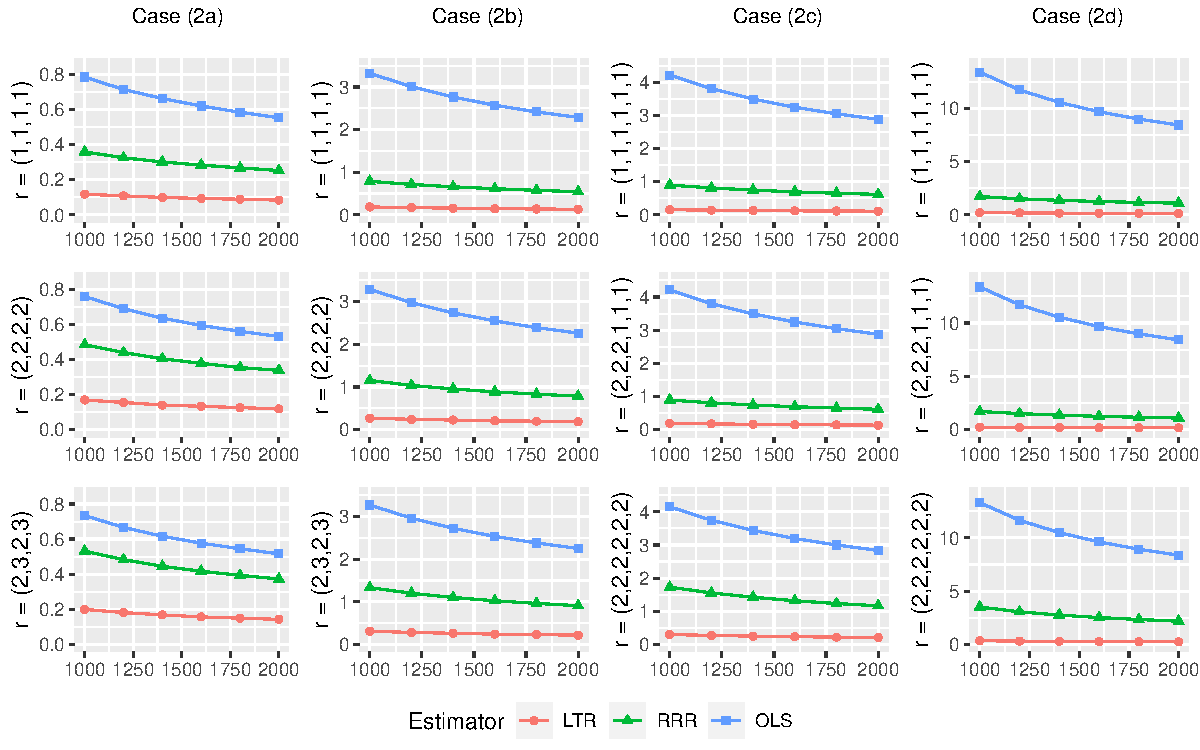
\includegraphics[width=\textwidth]{simulation1.pdf}
	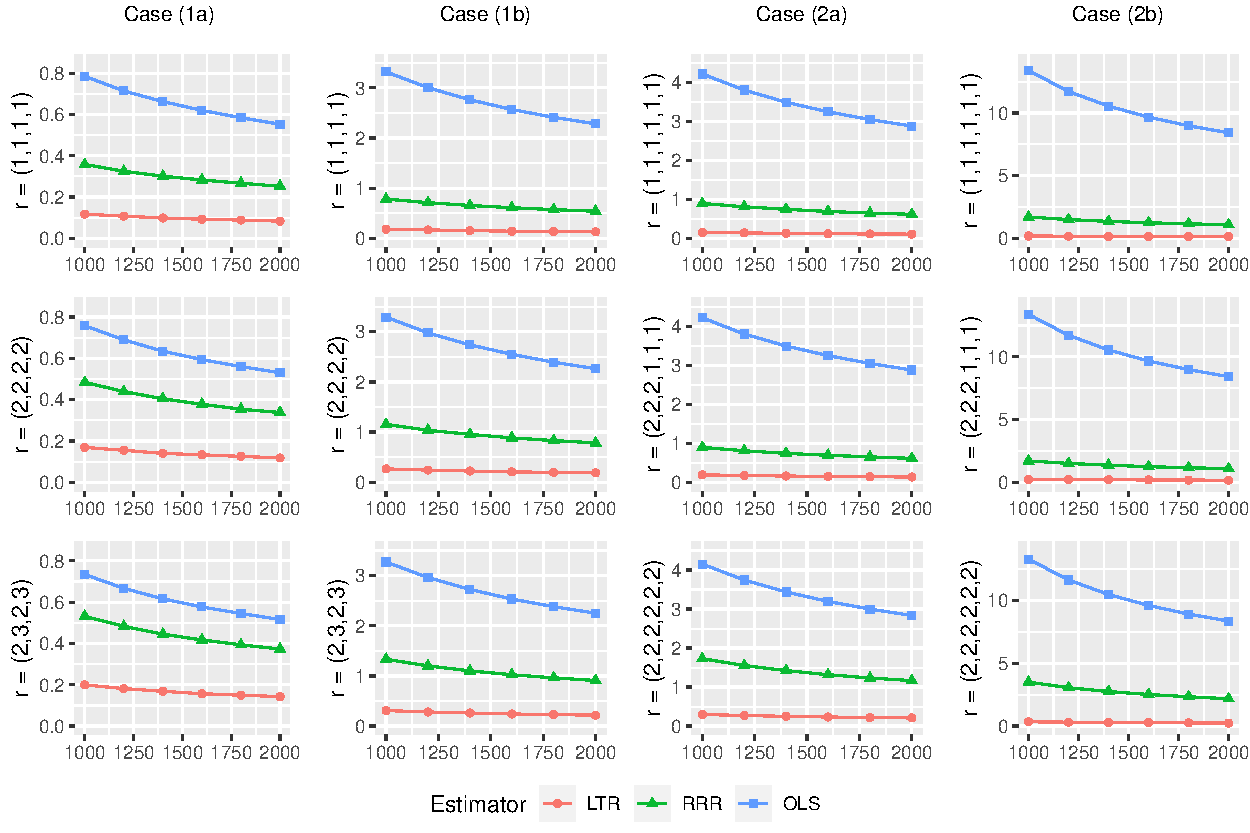
\includegraphics[width=\textwidth]{Rplot_sim1.pdf}
	\caption{Average estimation error of LTR, OLS and RRR estimators for data generated with different $d$,  $p_i$'s and multilinear ranks.}\label{fg:simulation1}
\end{figure} 

\begin{table}[t]
	\begin{center}
		\begin{tabular}{c|c|c|c}
			\hline
			Case & $d$ & Fixed Parameter & Varying Parameter\\
			\hline
			(a) & 2 & $T=500$, $\bm{r}=(2,2,2,2)$ & $p_1=p_2=5,7,9,10,11$\\
			\hline
			(b) & 2 & $p_1=p_2=8$, $\bm{r}=(2,2,2,2)$ & $T=200,400,600,800,1000$\\
			\hline
			\multirow{2}*{(c)} & \multirow{2}*{2} & \multirow{2}*{$p_1=p_2=8$, $T=500$} & $\bm{r}=(1,1,1,1),(1,2,1,2)$,\\
			&&&$(2,2,2,2,2),(2,3,2,3),(3,3,3,3)$\\
			\hline
			(d) & 2 & $p=144$, $T=1000$, $\bm{r}=(1,1,1,1)$ & $p_1=3,4,6,8,12$\\
			\hline
			(e) & 3  & $T=1000$, $\bm{r}=(2,2,2,2,2,2)$ & $\bm{p}=(4,4,4), (4,4,5),(4,5,5),(5,5,5),(5,5,6)$\\
			\hline
			(f) & 3 & $\bm{p}=(5,5,5)$, $\bm{r}=(2,2,2,2,2,2)$ & $T=600,800,1000,1200,1400$\\
			\hline
			\multirow{2}*{(g)} & \multirow{2}*{3} & \multirow{2}*{$\bm{p}=(5,5,5)$, $T=1000$} & $\bm{r}=(1,1,1,1,1,1),(1,1,2,1,1,2)$\\
			&&& $(1,2,2,1,2,2),(2,2,2,2,2,2),(2,2,3,2,2,3)$\\
			\hline
			\multirow{2}*{(h)} & \multirow{2}*{3} & $p=144$, $T=1000$, & $\bm{p}=(2,2,36),(3,3,16)$,\\
			&& $\bm{r}=(1,1,1,1,1,1)$& $(4,4,9),(3,4,12),(4,6,6)$\\
			\hline
		\end{tabular}
	\end{center}
	\caption{Parameter setting for eight cases with different varying parameters, where $\bm{p}=(p_1,\dots, p_d)$ and $\bm{r}=(r_1,\dots, r_{2d})$.\label{tab1}}
\end{table}

\begin{figure}
	\centering
%	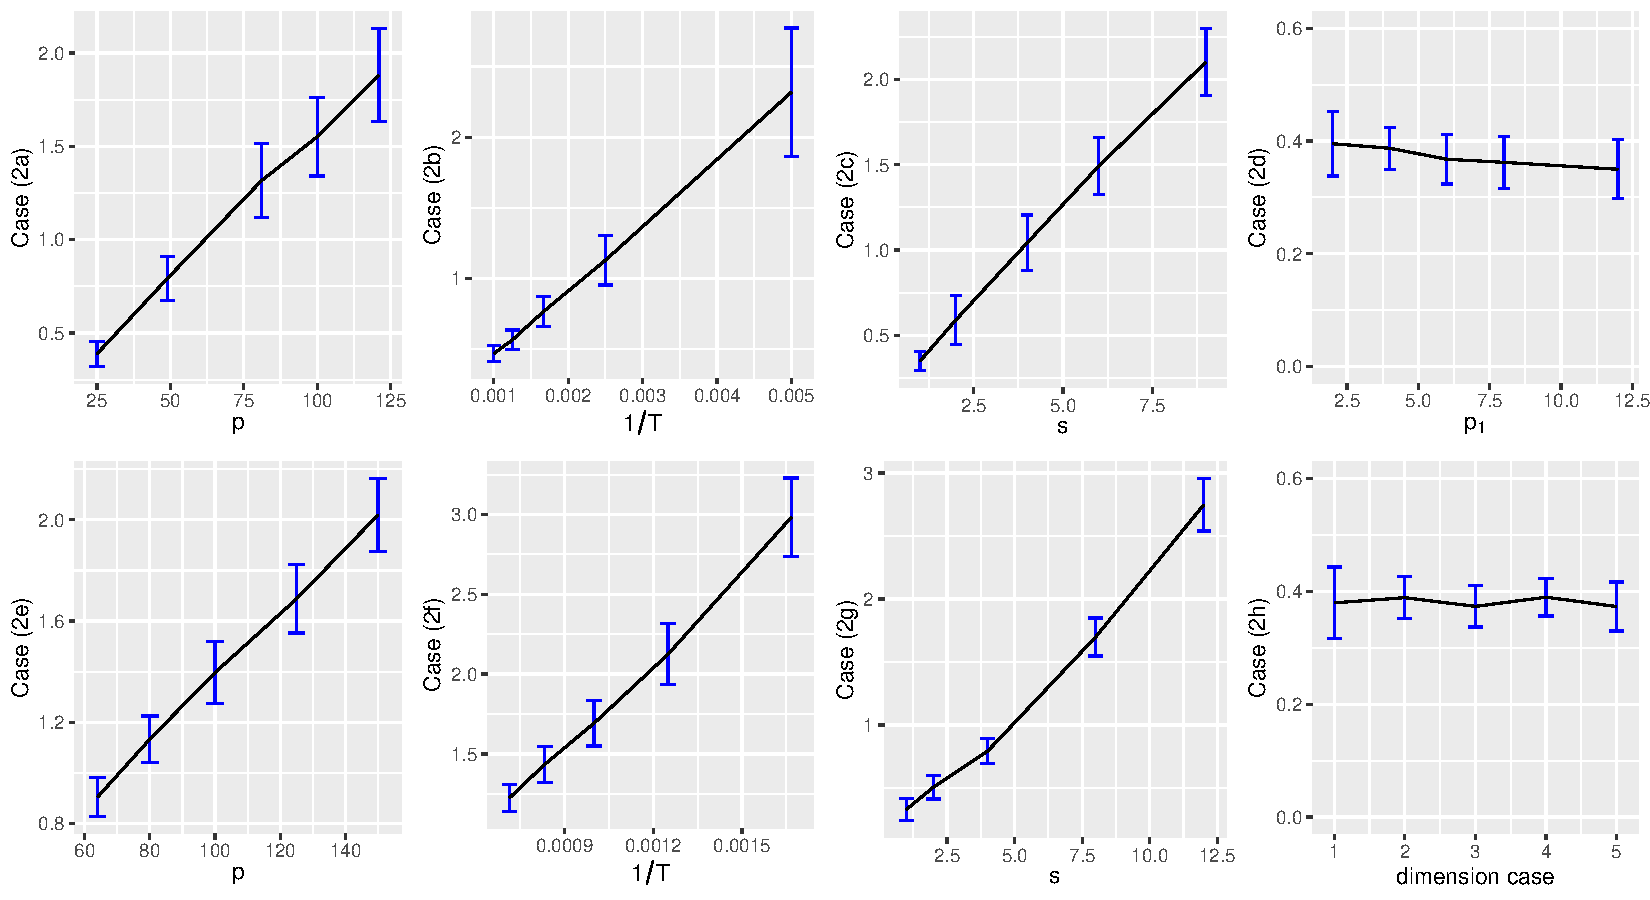
\includegraphics[width=\textwidth]{simulation2.pdf}
    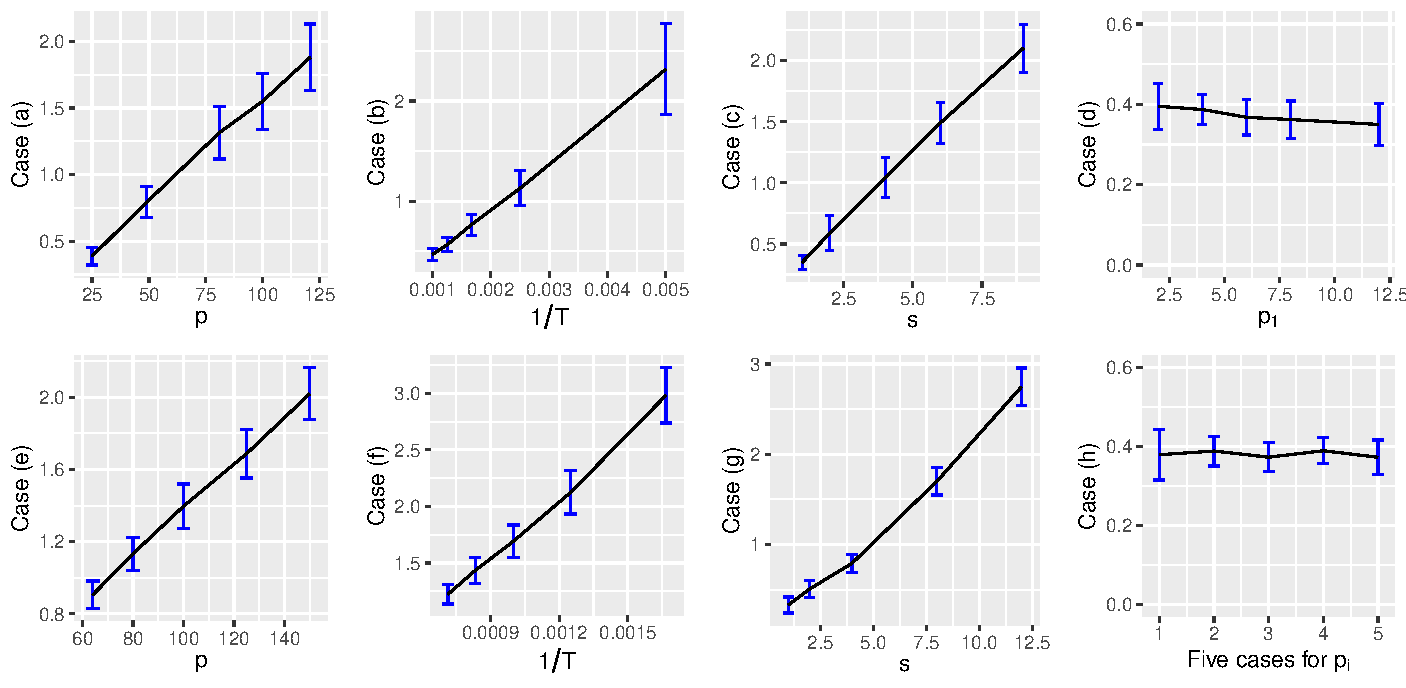
\includegraphics[width=\textwidth]{Rplot_sim2.pdf}
    \vspace{-12mm}
	\caption{Average squared estimation error for the SSN estimator for eight cases with different varying parameters. The error bars in each panel represent $\pm$ one standard deviation.}\label{fg:simulation2}
\end{figure}

\begin{figure}[t!]
	\centering
%	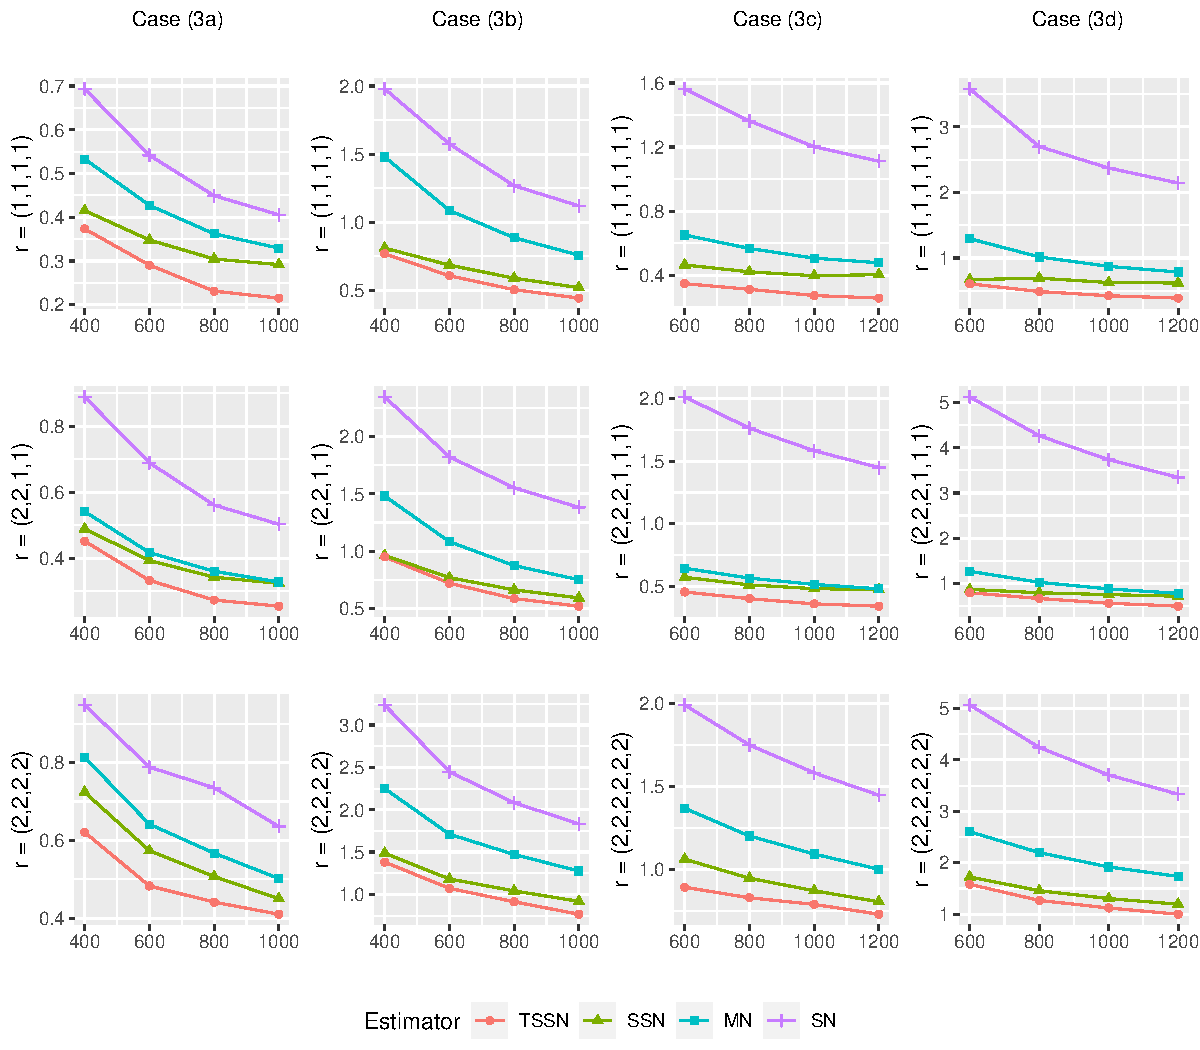
\includegraphics[width=\textwidth]{simulation3.pdf}
    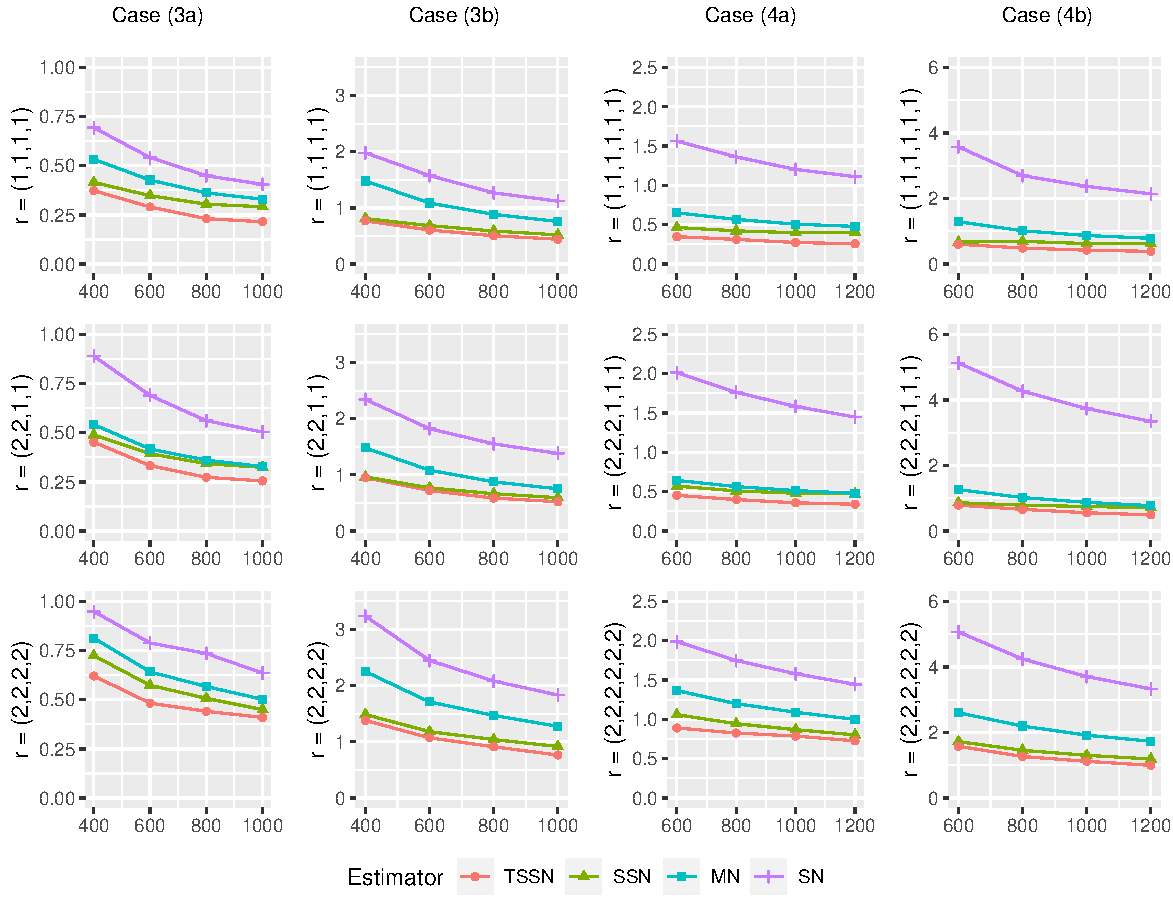
\includegraphics[width=\textwidth]{Rplot_sim3.pdf}
	\caption{Average estimation error for TSSN, SSN, MN, and SN estimators for data generated with different $d$,  $p_i$'s and multilinear ranks.}\label{fg:simulation3}
\end{figure}

%%%%%%%%%%%%%%%%%%%%%%%%%%%%%%%%%%%%%%%%%%%%%%%%%%%%%%%%%%%%%%%%%%%%%%%
\newpage
\clearpage

\begin{figure}[t]
	\begin{center}
		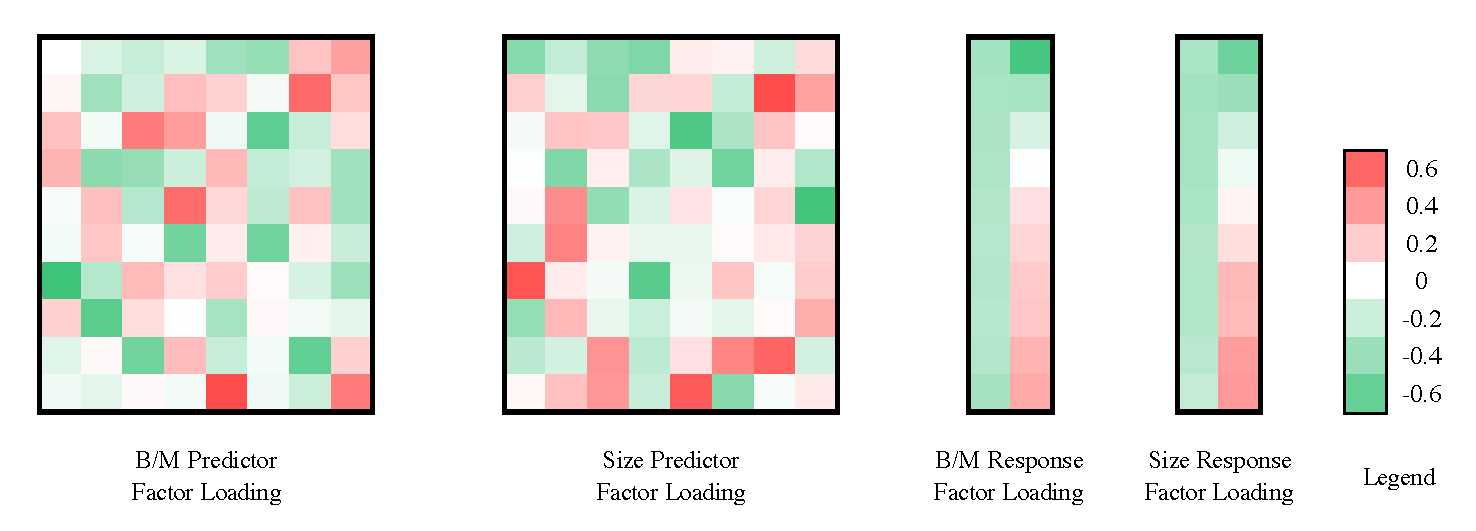
\includegraphics[width=\linewidth]{factor_loading1.pdf}
		\vspace{-15mm}
		\caption{TSSN estimates of predictor and response factor matrices for $10\times 10$  matrix-valued portfolio return series. From left to right: $\bm{\widetilde{U}}_1, \bm{\widetilde{U}}_2, \bm{\widetilde{U}}_3$ and $\bm{\widetilde{U}}_4$.}
		\label{fig:factor1}
	\end{center}
\end{figure}


\begin{table}%\vspace{-1cm}
	\begin{center}
		\begin{tabular}{cc|rrrrrrrccc}
			\hline\hline
			&\multirow{2}{*}{Model} & \multirow{2}{*}{VAR} & \multirow{2}{*}{VFM} & \multirow{2}{*}{MAR} & \multirow{2}{*}{MFM} && \multicolumn{2}{c}{LRTAR} && \multirow{2}{*}{Best} & \multirow{2}{*}{Worst}\\
			\cline{8-9}
			&&&&&& & \multicolumn{1}{c}{SSN} & TSSN &&&\\
			\hline
			\multirow{2}{*}{In-sample}& $\ell_2$ norm & \bf{31.61} & 35.85 & 34.12 & 35.86 && 33.18 & 33.38 && VAR & MFM\\
			& $\ell_0$ norm & \bf{8.09} & 9.23 & 9.12 & 9.24 && 8.84 & 8.89 && VAR & MFM\\
			\hline
			\multirow{2}{*}{Out-of-sample}& $\ell_2$ norm & 39.84 & 39.11 & 35.26 & 38.53 && 32.60 & \bf{31.47} && TSSN & VAR\\
			& $\ell_\infty$ norm & 11.98 & 12.30 & 11.47 & 11.00 &&  9.53 & \bf{9.33} && TSSN & VFM\\
			\hline
		\end{tabular}
		\caption{Average in-sample forecasting error and out-of-sample rolling forecasting error for $10\times 10$ matrix-valued portfolio return series. The best cases are marked in bold.}
		\label{tbl:in-sample-error}
	\end{center}
\end{table}

\clearpage
\newpage

\begin{figure}
	\begin{center}
		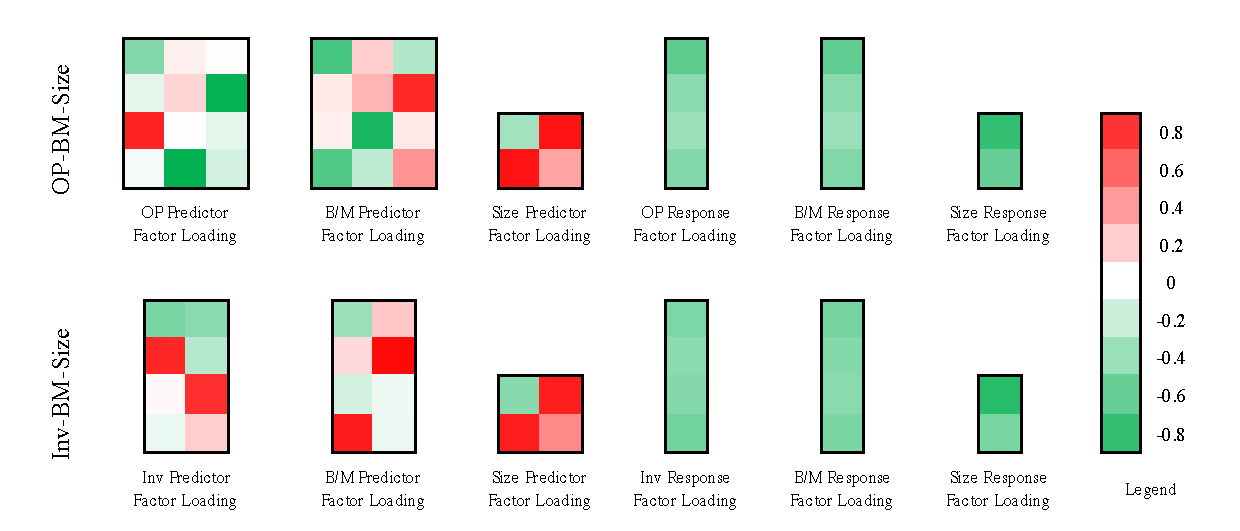
\includegraphics[width=\textwidth]{factor_loading2.pdf}
	\end{center}
	\vspace{-1cm}
	\caption{TSSN estimates of predictor and response factor matrices for $4\times 4\times 2$ tensor-valued portfolio return series. From left to right: $\bm{\widetilde{U}}_1, \bm{\widetilde{U}}_2, \bm{\widetilde{U}}_3$, $\bm{\widetilde{U}}_4$, $\bm{\widetilde{U}}_5$ and $\bm{\widetilde{U}}_6$.}
	\label{fig:factor2}
\end{figure}

\begin{table}
	\begin{center}
		\begin{tabular}{cc|rrrrrrrccc}
			\hline\hline
			&\multirow{2}{*}{Model} & \multirow{2}{*}{VAR} & \multirow{2}{*}{VFM} & \multirow{2}{*}{MTAR} & \multirow{2}{*}{TFM} && \multicolumn{2}{c}{LRTAR} && \multirow{2}{*}{Best} & \multirow{2}{*}{Worst}\\
			\cline{8-9}
			&&&&&&& \multicolumn{1}{c}{SSN} & TSSN &&&\\
			\hline
			\multicolumn{12}{c}{OP-BM-Size $4\times 4\times 2$ series}\\
			\hline
			\multirow{2}{*}{In-sample}& $\ell_2$ norm & \bf{19.53} & 20.08 & 19.89 & 20.09 && 19.69 & 19.70 && VAR & TFM\\
			& $\ell_0$ norm & \bf{7.67} & 7.91 & 7.85 & 7.92 && 7.76 & 7.77 && VAR & TFM\\
			\hline
			\multirow{2}{*}{Out-of-sample}& $\ell_2$ norm & 22.27 & 20.17 & 20.50 & 20.11 && 20.32 & \bf{19.95} && TSSN & VAR\\
			& $\ell_\infty$ norm & 10.38 & 10.04 & 9.86 & 10.03 && \bf{9.29} & 9.35 && SSN & VAR\\
			\hline
			\multicolumn{12}{c}{Inv-BM-Size $4\times 4\times 2$ series}\\
			\hline
			\multirow{2}{*}{In-sample}& $\ell_2$ norm & \bf{16.80} & 17.10 & 17.05 & 17.11 && 16.86 & 16.88  && VAR & TFM\\
			& $\ell_0$ norm & \bf{6.25} & 6.40 & 6.38 & 6.41 && 6.31 & 6.32  && VAR & TFM\\
			\hline
			\multirow{2}{*}{Out-of-sample} & $\ell_2$ norm & 18.70 & 17.70 & 16.89 & 17.67 && \bf{16.11} & 16.29 && SSN & VAR\\
			& $\ell_\infty$ norm & 7.42 & 7.37 & 6.79 & 7.33 && 6.62 & \bf{6.43} && TSSN & VAR\\
			\hline
		\end{tabular}
		\caption{Average in-sample forecasting error and out-of-sample rolling forecasting error for $4\times 4\times 2$ tensor-valued portfolio return series. The best cases are marked in bold.}
		\label{tbl:in-sample-error2}
	\end{center}
\end{table}


\end{document}
